\batchmode
\documentclass[twoside]{article}

% Packages required by doxygen
\usepackage{fixltx2e}
\usepackage{calc}
\usepackage{doxygen}
\usepackage[export]{adjustbox} % also loads graphicx
\usepackage{graphicx}
\usepackage[utf8]{inputenc}
\usepackage{makeidx}
\usepackage{multicol}
\usepackage{multirow}
\PassOptionsToPackage{warn}{textcomp}
\usepackage{textcomp}
\usepackage[nointegrals]{wasysym}
\usepackage[table]{xcolor}

% Font selection
\usepackage[T1]{fontenc}
\usepackage[scaled=.90]{helvet}
\usepackage{courier}
\usepackage{amssymb}
\usepackage{sectsty}
\renewcommand{\familydefault}{\sfdefault}
\allsectionsfont{%
  \fontseries{bc}\selectfont%
  \color{darkgray}%
}
\renewcommand{\DoxyLabelFont}{%
  \fontseries{bc}\selectfont%
  \color{darkgray}%
}
\newcommand{\+}{\discretionary{\mbox{\scriptsize$\hookleftarrow$}}{}{}}

% Page & text layout
\usepackage{geometry}
\geometry{%
  a4paper,%
  top=2.5cm,%
  bottom=2.5cm,%
  left=2.5cm,%
  right=2.5cm%
}
\tolerance=750
\hfuzz=15pt
\hbadness=750
\setlength{\emergencystretch}{15pt}
\setlength{\parindent}{0cm}
\setlength{\parskip}{0.2cm}
\makeatletter
\renewcommand{\paragraph}{%
  \@startsection{paragraph}{4}{0ex}{-1.0ex}{1.0ex}{%
    \normalfont\normalsize\bfseries\SS@parafont%
  }%
}
\renewcommand{\subparagraph}{%
  \@startsection{subparagraph}{5}{0ex}{-1.0ex}{1.0ex}{%
    \normalfont\normalsize\bfseries\SS@subparafont%
  }%
}
\makeatother

% Headers & footers
\usepackage{fancyhdr}
\pagestyle{fancyplain}
\fancyhead[LE]{\fancyplain{}{\bfseries\thepage}}
\fancyhead[CE]{\fancyplain{}{}}
\fancyhead[RE]{\fancyplain{}{\bfseries\leftmark}}
\fancyhead[LO]{\fancyplain{}{\bfseries\rightmark}}
\fancyhead[CO]{\fancyplain{}{}}
\fancyhead[RO]{\fancyplain{}{\bfseries\thepage}}
\fancyfoot[LE]{\fancyplain{}{}}
\fancyfoot[CE]{\fancyplain{}{}}
\fancyfoot[RE]{\fancyplain{}{\bfseries\scriptsize Generated on Sat Jun 6 2015 13\+:05\+:15 for Delta\+Robot by Doxygen }}
\fancyfoot[LO]{\fancyplain{}{\bfseries\scriptsize Generated on Sat Jun 6 2015 13\+:05\+:15 for Delta\+Robot by Doxygen }}
\fancyfoot[CO]{\fancyplain{}{}}
\fancyfoot[RO]{\fancyplain{}{}}
\renewcommand{\footrulewidth}{0.4pt}
\renewcommand{\sectionmark}[1]{%
  \markright{\thesection\ #1}%
}

% Indices & bibliography
\usepackage{natbib}
\usepackage[titles]{tocloft}
\setcounter{tocdepth}{3}
\setcounter{secnumdepth}{5}
\makeindex

% Hyperlinks (required, but should be loaded last)
\usepackage{ifpdf}
\ifpdf
  \usepackage[pdftex,pagebackref=true]{hyperref}
\else
  \usepackage[ps2pdf,pagebackref=true]{hyperref}
\fi
\hypersetup{%
  colorlinks=true,%
  linkcolor=blue,%
  citecolor=blue,%
  unicode%
}

% Custom commands
\newcommand{\clearemptydoublepage}{%
  \newpage{\pagestyle{empty}\cleardoublepage}%
}


%===== C O N T E N T S =====

\begin{document}

% Titlepage & ToC
\hypersetup{pageanchor=false,
             bookmarks=true,
             bookmarksnumbered=true,
             pdfencoding=unicode
            }
\pagenumbering{roman}
\begin{titlepage}
\vspace*{7cm}
\begin{center}%
{\Large Delta\+Robot \\[1ex]\large v0.\+4 }\\
\vspace*{1cm}
{\large Generated by Doxygen 1.8.9.1}\\
\vspace*{0.5cm}
{\small Sat Jun 6 2015 13:05:15}\\
\end{center}
\end{titlepage}
\tableofcontents
\pagenumbering{arabic}
\hypersetup{pageanchor=true}

%--- Begin generated contents ---
\section{Main Page}
\label{index}\hypertarget{index}{}This project is a Delta robot controller using Dynamixel \hyperlink{a00001}{A\+X12} servos.\+This type of robot can pick and place objects 
\section{Namespace Documentation}
\hypertarget{a00027}{}\subsection{Ui Namespace Reference}
\label{a00027}\index{Ui@{Ui}}


Namespace to work with a User Interface Qt Form.  




\subsubsection{Detailed Description}
Namespace to work with a User Interface Qt Form. 
\section{Class Documentation}
\hypertarget{a00001}{}\subsection{A\+X12 Class Reference}
\label{a00001}\index{A\+X12@{A\+X12}}


The \hyperlink{a00001}{A\+X12} class is used to control A\+X-\/12 motors from Dynamixel.  




{\ttfamily \#include $<$ax12.\+h$>$}



Collaboration diagram for A\+X12\+:\nopagebreak
\begin{figure}[H]
\begin{center}
\leavevmode
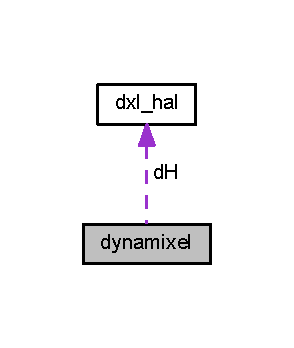
\includegraphics[width=141pt]{d5/d16/a00029}
\end{center}
\end{figure}
\subsubsection*{Public Types}
\begin{DoxyCompactItemize}
\item 
enum \hyperlink{a00001_a08d272b502d65464202a3aa97825aec0}{R\+O\+M} \{ \\*
\hyperlink{a00001_a08d272b502d65464202a3aa97825aec0afaeddb6fc62aacc16e88f98a77efbcff}{Model\+Number} = 0, 
\hyperlink{a00001_a08d272b502d65464202a3aa97825aec0a234de9d5194d6b6f4e45b854dbf1442d}{Version\+Firmware} = 2, 
\hyperlink{a00001_a08d272b502d65464202a3aa97825aec0ab2565d5698c9d943a8bcecf02b1389ad}{I\+D} = 3, 
\hyperlink{a00001_a08d272b502d65464202a3aa97825aec0afa8229ff24576bd10b061c259cc1146d}{Baud\+Rate} = 4, 
\\*
\hyperlink{a00001_a08d272b502d65464202a3aa97825aec0a1e7fa07a9a5a28584a287668a95dbb4f}{Return\+Delay\+Time} = 5, 
\hyperlink{a00001_a08d272b502d65464202a3aa97825aec0aae428847c3648681e8aae8f0a12c6880}{C\+W\+Angle\+Limit} = 6, 
\hyperlink{a00001_a08d272b502d65464202a3aa97825aec0ac631a1a4dfb22cd02e863fa19f509523}{C\+C\+W\+Angle\+Limit} = 8, 
\hyperlink{a00001_a08d272b502d65464202a3aa97825aec0aa9f1a3f67a0bf70f6e6530cac9f55153}{Highest\+Limit\+Temp} = 11, 
\\*
\hyperlink{a00001_a08d272b502d65464202a3aa97825aec0a75d2b929c12ad95dfe84b3214e5badd5}{Lowest\+Limit\+Voltage} = 12, 
\hyperlink{a00001_a08d272b502d65464202a3aa97825aec0a39bed5183cada3039894ec459e9cdba4}{Highest\+Limit\+Voltage} = 13, 
\hyperlink{a00001_a08d272b502d65464202a3aa97825aec0aa45ee204b37e8a8657bbb0be1f3f2ee5}{Max\+Torque} = 14, 
\hyperlink{a00001_a08d272b502d65464202a3aa97825aec0a1f50b233b75db417410a9ad75671c5f8}{Status\+Return\+Level} = 16, 
\\*
\hyperlink{a00001_a08d272b502d65464202a3aa97825aec0a69af7afba3f29c206407f802a6975dd1}{Alarm\+L\+E\+D} = 17, 
\hyperlink{a00001_a08d272b502d65464202a3aa97825aec0a017096d92de6aa9fa691df824cd21757}{Alarm\+Shutdown} = 18
 \}
\begin{DoxyCompactList}\small\item\em Contains all the E\+E\+P\+R\+O\+M directions enumeration. \end{DoxyCompactList}\item 
enum \hyperlink{a00001_a672068c48bbee921e5856cc44b1c81c1}{R\+A\+M} \{ \\*
\hyperlink{a00001_a672068c48bbee921e5856cc44b1c81c1ac4597f1de691116b512ae043da6ae7a3}{Torque\+Enable} = 24, 
\hyperlink{a00001_a672068c48bbee921e5856cc44b1c81c1af9d9ebff7bdb8cbb20edfac6f553f796}{L\+E\+D} = 25, 
\hyperlink{a00001_a672068c48bbee921e5856cc44b1c81c1ac2410c95fb1bb2343adc3d3b621cb1d0}{C\+W\+Compliance\+Margin} = 26, 
\hyperlink{a00001_a672068c48bbee921e5856cc44b1c81c1aa9e82bf2f003910708111a4ade3ec42d}{C\+C\+W\+Compliance\+Margin} = 27, 
\\*
\hyperlink{a00001_a672068c48bbee921e5856cc44b1c81c1a1dffe196ada84077dfbfcd72d31be8c8}{C\+W\+Compliance\+Slope} = 28, 
\hyperlink{a00001_a672068c48bbee921e5856cc44b1c81c1a624015aab9c06310e1f96bafe8f934a7}{C\+C\+W\+Compliance\+Slope} = 29, 
\hyperlink{a00001_a672068c48bbee921e5856cc44b1c81c1ae3d6ac0b56a8ab2b188f14545473cbef}{Goal\+Position} = 30, 
\hyperlink{a00001_a672068c48bbee921e5856cc44b1c81c1a77389ef2d6dc4bfe760357bd375d5284}{Moving\+Speed} = 32, 
\\*
\hyperlink{a00001_a672068c48bbee921e5856cc44b1c81c1adc48ae20914d1771097b17c08be83bbc}{Torque\+Limit} = 34, 
\hyperlink{a00001_a672068c48bbee921e5856cc44b1c81c1ac3714d28e016c704ea8451c18700dea8}{Present\+Position} = 36, 
\hyperlink{a00001_a672068c48bbee921e5856cc44b1c81c1a481b48fdf5e3609568bdbde19c32ef90}{Present\+Speed} = 38, 
\hyperlink{a00001_a672068c48bbee921e5856cc44b1c81c1a4acb9c359962b60a1dfc900550f4b2b2}{Present\+Load} = 40, 
\\*
\hyperlink{a00001_a672068c48bbee921e5856cc44b1c81c1a908c1a7f566782c4c258c779b5ca54cd}{Present\+Voltage} = 42, 
\hyperlink{a00001_a672068c48bbee921e5856cc44b1c81c1ae00a92c23c2af2faf19eb051424cf271}{Present\+Temperature} = 43, 
\hyperlink{a00001_a672068c48bbee921e5856cc44b1c81c1a426e2185243d7ae4213d048abbf56938}{Registered} = 44, 
\hyperlink{a00001_a672068c48bbee921e5856cc44b1c81c1a1649d49cd35bc3ebfdc8be06b61b7caf}{Moving} = 46, 
\\*
\hyperlink{a00001_a672068c48bbee921e5856cc44b1c81c1a67e9c5c73f91985138111a792458e5ad}{Lock} = 47, 
\hyperlink{a00001_a672068c48bbee921e5856cc44b1c81c1a491959069a5cf99cf49bd2fd9ea5ec92}{Punch} = 48
 \}
\begin{DoxyCompactList}\small\item\em Contains all the R\+A\+M directions enumerations. \end{DoxyCompactList}\end{DoxyCompactItemize}
\subsubsection*{Public Member Functions}
\begin{DoxyCompactItemize}
\item 
\hyperlink{a00001_ab7c557985e755d6119e5e2d979f928ae}{A\+X12} ()
\begin{DoxyCompactList}\small\item\em Default constructor. \end{DoxyCompactList}\item 
\hyperlink{a00001_a205be9b4dde785bd40b88f575a64f4d8}{A\+X12} (\hyperlink{a00004}{dynamixel} $\ast$\hyperlink{a00001_a16df7ccc0a8d3c585a93b6916734bb17}{\+\_\+dxl}, int \hyperlink{a00001_a08d272b502d65464202a3aa97825aec0ab2565d5698c9d943a8bcecf02b1389ad}{I\+D}=-\/1)
\begin{DoxyCompactList}\small\item\em Initializator constructor if I\+D == -\/1 no action is done. \end{DoxyCompactList}\item 
\hyperlink{a00001_a37b76666533323ec317f5156dbef2a89}{A\+X12} (const \hyperlink{a00001}{A\+X12} \&a)
\begin{DoxyCompactList}\small\item\em Copy constructor. \end{DoxyCompactList}\item 
\hyperlink{a00001_a5e9382e65479cdcb248f5303ac4c96d9}{$\sim$\+A\+X12} ()
\begin{DoxyCompactList}\small\item\em Default destructor. \end{DoxyCompactList}\item 
Q\+Vector$<$ int $>$ \hyperlink{a00001_a2fa05296aa57896a5cb0ef4ce0aa96f1}{connected\+I\+D} ()
\begin{DoxyCompactList}\small\item\em Returns all active servos;. \end{DoxyCompactList}\item 
double \hyperlink{a00001_a0bd930c81b7a9c088ecab789b3a7e525}{get\+Current\+Load} ()
\begin{DoxyCompactList}\small\item\em Returns the current load from -\/100\% to 100\%, 100\% is Clock\+Wise and -\/100\% is Counter\+Clock\+Wise. \end{DoxyCompactList}\item 
double \hyperlink{a00001_af9722b9c1f82fbfd97fe5e0a44369e8a}{get\+Current\+Pos} ()
\begin{DoxyCompactList}\small\item\em Returns the current position from 0º to 300º \end{DoxyCompactList}\item 
int \hyperlink{a00001_ab16fad4c8c034d56acce15fc9102f34d}{get\+Current\+Temp} ()
\begin{DoxyCompactList}\small\item\em Returns the current Temperature in Celsius. \end{DoxyCompactList}\item 
double \hyperlink{a00001_a23c7ed54716c4b144a68d801f324e3ef}{get\+Current\+Speed} ()
\begin{DoxyCompactList}\small\item\em Returns the current speed from -\/100\% to 100\%, 100\% is Clock\+Wise and -\/100\% is Counter\+Clock\+Wise. \end{DoxyCompactList}\item 
double \hyperlink{a00001_a9ef946bfc1ad4dce5fed4101ed321efe}{get\+Current\+Voltage} ()
\begin{DoxyCompactList}\small\item\em Returns the current voltage in Volts. \end{DoxyCompactList}\item 
int \hyperlink{a00001_a745ab1f31fa2cd8c7a5797aeb605cd0b}{get\+I\+D} ()
\begin{DoxyCompactList}\small\item\em To get the current I\+D. \end{DoxyCompactList}\item 
void \hyperlink{a00001_a6ef2e11a3b0bdb5015142ba04593a770}{set\+Compliance\+Slope} (uchar ccw, uchar cw)
\begin{DoxyCompactList}\small\item\em Sets the compliance slope. \end{DoxyCompactList}\item 
void \hyperlink{a00001_a74a5a89387f0f51e053f05a6c2c0b9c5}{set\+Dxl} (\hyperlink{a00004}{dynamixel} $\ast$dxl)
\begin{DoxyCompactList}\small\item\em Sets the dynamixel interface. \end{DoxyCompactList}\item 
void \hyperlink{a00001_a6b27a3c6314604b499d9fa47d180f5d3}{set\+Goal\+Position} (double goal)
\begin{DoxyCompactList}\small\item\em Sets the Goal\textquotesingle{}s position (in degrees) or speed depending on the mode. \end{DoxyCompactList}\item 
void \hyperlink{a00001_ab9fe5d0e2286985977985de6d84b1103}{set\+I\+D} (int \hyperlink{a00001_a08d272b502d65464202a3aa97825aec0ab2565d5698c9d943a8bcecf02b1389ad}{I\+D})
\begin{DoxyCompactList}\small\item\em To set a new I\+D. \end{DoxyCompactList}\item 
void \hyperlink{a00001_ac48405a5f4aa73c1f2d56f633dfbec50}{set\+Joint\+Mode} (bool mode)
\begin{DoxyCompactList}\small\item\em To set Joint/\+Wheel mode. \end{DoxyCompactList}\item 
void \hyperlink{a00001_a914864d133f8cbaf95594747aaff55f2}{set\+Min\+Max} (double min, double max)
\begin{DoxyCompactList}\small\item\em To set the minimum and maximum angle from 0 to 300º \end{DoxyCompactList}\item 
void \hyperlink{a00001_a120a8fb196ce724f118fd1774b658040}{set\+Radians} (bool rads)
\begin{DoxyCompactList}\small\item\em Sets the radians mode. \end{DoxyCompactList}\item 
void \hyperlink{a00001_a95428eea4d5165b81d80e4ab38e33b7b}{set\+Speed} (double speed)
\begin{DoxyCompactList}\small\item\em To set the maximum speed from 0\% to 100\% if joint mode or from -\/100\% to 100\% if wheel mode. \end{DoxyCompactList}\end{DoxyCompactItemize}
\subsubsection*{Private Attributes}
\begin{DoxyCompactItemize}
\item 
\hyperlink{a00004}{dynamixel} $\ast$ \hyperlink{a00001_a16df7ccc0a8d3c585a93b6916734bb17}{\+\_\+dxl}
\begin{DoxyCompactList}\small\item\em Contains the dynamixel comunication. \end{DoxyCompactList}\item 
int \hyperlink{a00001_a0ae2b35fee3d120075e1d8f1e2055804}{\+\_\+\+I\+D}
\begin{DoxyCompactList}\small\item\em Stores the current I\+D. \end{DoxyCompactList}\item 
bool \hyperlink{a00001_a2fd07e2e636003227a32d09d211bd6d4}{\+\_\+mode}
\begin{DoxyCompactList}\small\item\em True if we use the joint mode. \end{DoxyCompactList}\item 
bool \hyperlink{a00001_aba71492043d7a3226f0793db57372bec}{\+\_\+rads}
\begin{DoxyCompactList}\small\item\em True if the angle is returned in radians. \end{DoxyCompactList}\end{DoxyCompactItemize}


\subsubsection{Detailed Description}
The \hyperlink{a00001}{A\+X12} class is used to control A\+X-\/12 motors from Dynamixel. 

\subsubsection{Member Enumeration Documentation}
\hypertarget{a00001_a672068c48bbee921e5856cc44b1c81c1}{}\index{A\+X12@{A\+X12}!R\+A\+M@{R\+A\+M}}
\index{R\+A\+M@{R\+A\+M}!A\+X12@{A\+X12}}
\paragraph[{R\+A\+M}]{\setlength{\rightskip}{0pt plus 5cm}enum {\bf A\+X12\+::\+R\+A\+M}}\label{a00001_a672068c48bbee921e5856cc44b1c81c1}


Contains all the R\+A\+M directions enumerations. 

\begin{Desc}
\item[Enumerator]\par
\begin{description}
\index{Torque\+Enable@{Torque\+Enable}!A\+X12@{A\+X12}}\index{A\+X12@{A\+X12}!Torque\+Enable@{Torque\+Enable}}\item[{\em 
\hypertarget{a00001_a672068c48bbee921e5856cc44b1c81c1ac4597f1de691116b512ae043da6ae7a3}{}Torque\+Enable\label{a00001_a672068c48bbee921e5856cc44b1c81c1ac4597f1de691116b512ae043da6ae7a3}
}]\index{L\+E\+D@{L\+E\+D}!A\+X12@{A\+X12}}\index{A\+X12@{A\+X12}!L\+E\+D@{L\+E\+D}}\item[{\em 
\hypertarget{a00001_a672068c48bbee921e5856cc44b1c81c1af9d9ebff7bdb8cbb20edfac6f553f796}{}L\+E\+D\label{a00001_a672068c48bbee921e5856cc44b1c81c1af9d9ebff7bdb8cbb20edfac6f553f796}
}]\index{C\+W\+Compliance\+Margin@{C\+W\+Compliance\+Margin}!A\+X12@{A\+X12}}\index{A\+X12@{A\+X12}!C\+W\+Compliance\+Margin@{C\+W\+Compliance\+Margin}}\item[{\em 
\hypertarget{a00001_a672068c48bbee921e5856cc44b1c81c1ac2410c95fb1bb2343adc3d3b621cb1d0}{}C\+W\+Compliance\+Margin\label{a00001_a672068c48bbee921e5856cc44b1c81c1ac2410c95fb1bb2343adc3d3b621cb1d0}
}]\index{C\+C\+W\+Compliance\+Margin@{C\+C\+W\+Compliance\+Margin}!A\+X12@{A\+X12}}\index{A\+X12@{A\+X12}!C\+C\+W\+Compliance\+Margin@{C\+C\+W\+Compliance\+Margin}}\item[{\em 
\hypertarget{a00001_a672068c48bbee921e5856cc44b1c81c1aa9e82bf2f003910708111a4ade3ec42d}{}C\+C\+W\+Compliance\+Margin\label{a00001_a672068c48bbee921e5856cc44b1c81c1aa9e82bf2f003910708111a4ade3ec42d}
}]\index{C\+W\+Compliance\+Slope@{C\+W\+Compliance\+Slope}!A\+X12@{A\+X12}}\index{A\+X12@{A\+X12}!C\+W\+Compliance\+Slope@{C\+W\+Compliance\+Slope}}\item[{\em 
\hypertarget{a00001_a672068c48bbee921e5856cc44b1c81c1a1dffe196ada84077dfbfcd72d31be8c8}{}C\+W\+Compliance\+Slope\label{a00001_a672068c48bbee921e5856cc44b1c81c1a1dffe196ada84077dfbfcd72d31be8c8}
}]\index{C\+C\+W\+Compliance\+Slope@{C\+C\+W\+Compliance\+Slope}!A\+X12@{A\+X12}}\index{A\+X12@{A\+X12}!C\+C\+W\+Compliance\+Slope@{C\+C\+W\+Compliance\+Slope}}\item[{\em 
\hypertarget{a00001_a672068c48bbee921e5856cc44b1c81c1a624015aab9c06310e1f96bafe8f934a7}{}C\+C\+W\+Compliance\+Slope\label{a00001_a672068c48bbee921e5856cc44b1c81c1a624015aab9c06310e1f96bafe8f934a7}
}]\index{Goal\+Position@{Goal\+Position}!A\+X12@{A\+X12}}\index{A\+X12@{A\+X12}!Goal\+Position@{Goal\+Position}}\item[{\em 
\hypertarget{a00001_a672068c48bbee921e5856cc44b1c81c1ae3d6ac0b56a8ab2b188f14545473cbef}{}Goal\+Position\label{a00001_a672068c48bbee921e5856cc44b1c81c1ae3d6ac0b56a8ab2b188f14545473cbef}
}]\index{Moving\+Speed@{Moving\+Speed}!A\+X12@{A\+X12}}\index{A\+X12@{A\+X12}!Moving\+Speed@{Moving\+Speed}}\item[{\em 
\hypertarget{a00001_a672068c48bbee921e5856cc44b1c81c1a77389ef2d6dc4bfe760357bd375d5284}{}Moving\+Speed\label{a00001_a672068c48bbee921e5856cc44b1c81c1a77389ef2d6dc4bfe760357bd375d5284}
}]\index{Torque\+Limit@{Torque\+Limit}!A\+X12@{A\+X12}}\index{A\+X12@{A\+X12}!Torque\+Limit@{Torque\+Limit}}\item[{\em 
\hypertarget{a00001_a672068c48bbee921e5856cc44b1c81c1adc48ae20914d1771097b17c08be83bbc}{}Torque\+Limit\label{a00001_a672068c48bbee921e5856cc44b1c81c1adc48ae20914d1771097b17c08be83bbc}
}]\index{Present\+Position@{Present\+Position}!A\+X12@{A\+X12}}\index{A\+X12@{A\+X12}!Present\+Position@{Present\+Position}}\item[{\em 
\hypertarget{a00001_a672068c48bbee921e5856cc44b1c81c1ac3714d28e016c704ea8451c18700dea8}{}Present\+Position\label{a00001_a672068c48bbee921e5856cc44b1c81c1ac3714d28e016c704ea8451c18700dea8}
}]\index{Present\+Speed@{Present\+Speed}!A\+X12@{A\+X12}}\index{A\+X12@{A\+X12}!Present\+Speed@{Present\+Speed}}\item[{\em 
\hypertarget{a00001_a672068c48bbee921e5856cc44b1c81c1a481b48fdf5e3609568bdbde19c32ef90}{}Present\+Speed\label{a00001_a672068c48bbee921e5856cc44b1c81c1a481b48fdf5e3609568bdbde19c32ef90}
}]\index{Present\+Load@{Present\+Load}!A\+X12@{A\+X12}}\index{A\+X12@{A\+X12}!Present\+Load@{Present\+Load}}\item[{\em 
\hypertarget{a00001_a672068c48bbee921e5856cc44b1c81c1a4acb9c359962b60a1dfc900550f4b2b2}{}Present\+Load\label{a00001_a672068c48bbee921e5856cc44b1c81c1a4acb9c359962b60a1dfc900550f4b2b2}
}]\index{Present\+Voltage@{Present\+Voltage}!A\+X12@{A\+X12}}\index{A\+X12@{A\+X12}!Present\+Voltage@{Present\+Voltage}}\item[{\em 
\hypertarget{a00001_a672068c48bbee921e5856cc44b1c81c1a908c1a7f566782c4c258c779b5ca54cd}{}Present\+Voltage\label{a00001_a672068c48bbee921e5856cc44b1c81c1a908c1a7f566782c4c258c779b5ca54cd}
}]\index{Present\+Temperature@{Present\+Temperature}!A\+X12@{A\+X12}}\index{A\+X12@{A\+X12}!Present\+Temperature@{Present\+Temperature}}\item[{\em 
\hypertarget{a00001_a672068c48bbee921e5856cc44b1c81c1ae00a92c23c2af2faf19eb051424cf271}{}Present\+Temperature\label{a00001_a672068c48bbee921e5856cc44b1c81c1ae00a92c23c2af2faf19eb051424cf271}
}]\index{Registered@{Registered}!A\+X12@{A\+X12}}\index{A\+X12@{A\+X12}!Registered@{Registered}}\item[{\em 
\hypertarget{a00001_a672068c48bbee921e5856cc44b1c81c1a426e2185243d7ae4213d048abbf56938}{}Registered\label{a00001_a672068c48bbee921e5856cc44b1c81c1a426e2185243d7ae4213d048abbf56938}
}]\index{Moving@{Moving}!A\+X12@{A\+X12}}\index{A\+X12@{A\+X12}!Moving@{Moving}}\item[{\em 
\hypertarget{a00001_a672068c48bbee921e5856cc44b1c81c1a1649d49cd35bc3ebfdc8be06b61b7caf}{}Moving\label{a00001_a672068c48bbee921e5856cc44b1c81c1a1649d49cd35bc3ebfdc8be06b61b7caf}
}]\index{Lock@{Lock}!A\+X12@{A\+X12}}\index{A\+X12@{A\+X12}!Lock@{Lock}}\item[{\em 
\hypertarget{a00001_a672068c48bbee921e5856cc44b1c81c1a67e9c5c73f91985138111a792458e5ad}{}Lock\label{a00001_a672068c48bbee921e5856cc44b1c81c1a67e9c5c73f91985138111a792458e5ad}
}]\index{Punch@{Punch}!A\+X12@{A\+X12}}\index{A\+X12@{A\+X12}!Punch@{Punch}}\item[{\em 
\hypertarget{a00001_a672068c48bbee921e5856cc44b1c81c1a491959069a5cf99cf49bd2fd9ea5ec92}{}Punch\label{a00001_a672068c48bbee921e5856cc44b1c81c1a491959069a5cf99cf49bd2fd9ea5ec92}
}]\end{description}
\end{Desc}

\begin{DoxyCode}
00058     \{
00059         \hyperlink{a00001_a672068c48bbee921e5856cc44b1c81c1ac4597f1de691116b512ae043da6ae7a3}{TorqueEnable}        = 24,
00060         \hyperlink{a00001_a672068c48bbee921e5856cc44b1c81c1af9d9ebff7bdb8cbb20edfac6f553f796}{LED}                 = 25,
00061         \hyperlink{a00001_a672068c48bbee921e5856cc44b1c81c1ac2410c95fb1bb2343adc3d3b621cb1d0}{CWComplianceMargin}  = 26,
00062         \hyperlink{a00001_a672068c48bbee921e5856cc44b1c81c1aa9e82bf2f003910708111a4ade3ec42d}{CCWComplianceMargin} = 27,
00063         \hyperlink{a00001_a672068c48bbee921e5856cc44b1c81c1a1dffe196ada84077dfbfcd72d31be8c8}{CWComplianceSlope}   = 28,
00064         \hyperlink{a00001_a672068c48bbee921e5856cc44b1c81c1a624015aab9c06310e1f96bafe8f934a7}{CCWComplianceSlope}  = 29,
00065         \hyperlink{a00001_a672068c48bbee921e5856cc44b1c81c1ae3d6ac0b56a8ab2b188f14545473cbef}{GoalPosition}        = 30,
00066         \hyperlink{a00001_a672068c48bbee921e5856cc44b1c81c1a77389ef2d6dc4bfe760357bd375d5284}{MovingSpeed}         = 32,
00067         \hyperlink{a00001_a672068c48bbee921e5856cc44b1c81c1adc48ae20914d1771097b17c08be83bbc}{TorqueLimit}         = 34,
00068         \hyperlink{a00001_a672068c48bbee921e5856cc44b1c81c1ac3714d28e016c704ea8451c18700dea8}{PresentPosition}     = 36,
00069         \hyperlink{a00001_a672068c48bbee921e5856cc44b1c81c1a481b48fdf5e3609568bdbde19c32ef90}{PresentSpeed}        = 38,
00070         \hyperlink{a00001_a672068c48bbee921e5856cc44b1c81c1a4acb9c359962b60a1dfc900550f4b2b2}{PresentLoad}         = 40,
00071         \hyperlink{a00001_a672068c48bbee921e5856cc44b1c81c1a908c1a7f566782c4c258c779b5ca54cd}{PresentVoltage}      = 42,
00072         \hyperlink{a00001_a672068c48bbee921e5856cc44b1c81c1ae00a92c23c2af2faf19eb051424cf271}{PresentTemperature}  = 43,
00073         \hyperlink{a00001_a672068c48bbee921e5856cc44b1c81c1a426e2185243d7ae4213d048abbf56938}{Registered}          = 44,
00074         \hyperlink{a00001_a672068c48bbee921e5856cc44b1c81c1a1649d49cd35bc3ebfdc8be06b61b7caf}{Moving}              = 46,
00075         \hyperlink{a00001_a672068c48bbee921e5856cc44b1c81c1a67e9c5c73f91985138111a792458e5ad}{Lock}                = 47,
00076         \hyperlink{a00001_a672068c48bbee921e5856cc44b1c81c1a491959069a5cf99cf49bd2fd9ea5ec92}{Punch}               = 48
00077         
00078     \};   
\end{DoxyCode}
\hypertarget{a00001_a08d272b502d65464202a3aa97825aec0}{}\index{A\+X12@{A\+X12}!R\+O\+M@{R\+O\+M}}
\index{R\+O\+M@{R\+O\+M}!A\+X12@{A\+X12}}
\paragraph[{R\+O\+M}]{\setlength{\rightskip}{0pt plus 5cm}enum {\bf A\+X12\+::\+R\+O\+M}}\label{a00001_a08d272b502d65464202a3aa97825aec0}


Contains all the E\+E\+P\+R\+O\+M directions enumeration. 

\begin{Desc}
\item[Enumerator]\par
\begin{description}
\index{Model\+Number@{Model\+Number}!A\+X12@{A\+X12}}\index{A\+X12@{A\+X12}!Model\+Number@{Model\+Number}}\item[{\em 
\hypertarget{a00001_a08d272b502d65464202a3aa97825aec0afaeddb6fc62aacc16e88f98a77efbcff}{}Model\+Number\label{a00001_a08d272b502d65464202a3aa97825aec0afaeddb6fc62aacc16e88f98a77efbcff}
}]\index{Version\+Firmware@{Version\+Firmware}!A\+X12@{A\+X12}}\index{A\+X12@{A\+X12}!Version\+Firmware@{Version\+Firmware}}\item[{\em 
\hypertarget{a00001_a08d272b502d65464202a3aa97825aec0a234de9d5194d6b6f4e45b854dbf1442d}{}Version\+Firmware\label{a00001_a08d272b502d65464202a3aa97825aec0a234de9d5194d6b6f4e45b854dbf1442d}
}]\index{I\+D@{I\+D}!A\+X12@{A\+X12}}\index{A\+X12@{A\+X12}!I\+D@{I\+D}}\item[{\em 
\hypertarget{a00001_a08d272b502d65464202a3aa97825aec0ab2565d5698c9d943a8bcecf02b1389ad}{}I\+D\label{a00001_a08d272b502d65464202a3aa97825aec0ab2565d5698c9d943a8bcecf02b1389ad}
}]\index{Baud\+Rate@{Baud\+Rate}!A\+X12@{A\+X12}}\index{A\+X12@{A\+X12}!Baud\+Rate@{Baud\+Rate}}\item[{\em 
\hypertarget{a00001_a08d272b502d65464202a3aa97825aec0afa8229ff24576bd10b061c259cc1146d}{}Baud\+Rate\label{a00001_a08d272b502d65464202a3aa97825aec0afa8229ff24576bd10b061c259cc1146d}
}]\index{Return\+Delay\+Time@{Return\+Delay\+Time}!A\+X12@{A\+X12}}\index{A\+X12@{A\+X12}!Return\+Delay\+Time@{Return\+Delay\+Time}}\item[{\em 
\hypertarget{a00001_a08d272b502d65464202a3aa97825aec0a1e7fa07a9a5a28584a287668a95dbb4f}{}Return\+Delay\+Time\label{a00001_a08d272b502d65464202a3aa97825aec0a1e7fa07a9a5a28584a287668a95dbb4f}
}]\index{C\+W\+Angle\+Limit@{C\+W\+Angle\+Limit}!A\+X12@{A\+X12}}\index{A\+X12@{A\+X12}!C\+W\+Angle\+Limit@{C\+W\+Angle\+Limit}}\item[{\em 
\hypertarget{a00001_a08d272b502d65464202a3aa97825aec0aae428847c3648681e8aae8f0a12c6880}{}C\+W\+Angle\+Limit\label{a00001_a08d272b502d65464202a3aa97825aec0aae428847c3648681e8aae8f0a12c6880}
}]\index{C\+C\+W\+Angle\+Limit@{C\+C\+W\+Angle\+Limit}!A\+X12@{A\+X12}}\index{A\+X12@{A\+X12}!C\+C\+W\+Angle\+Limit@{C\+C\+W\+Angle\+Limit}}\item[{\em 
\hypertarget{a00001_a08d272b502d65464202a3aa97825aec0ac631a1a4dfb22cd02e863fa19f509523}{}C\+C\+W\+Angle\+Limit\label{a00001_a08d272b502d65464202a3aa97825aec0ac631a1a4dfb22cd02e863fa19f509523}
}]\index{Highest\+Limit\+Temp@{Highest\+Limit\+Temp}!A\+X12@{A\+X12}}\index{A\+X12@{A\+X12}!Highest\+Limit\+Temp@{Highest\+Limit\+Temp}}\item[{\em 
\hypertarget{a00001_a08d272b502d65464202a3aa97825aec0aa9f1a3f67a0bf70f6e6530cac9f55153}{}Highest\+Limit\+Temp\label{a00001_a08d272b502d65464202a3aa97825aec0aa9f1a3f67a0bf70f6e6530cac9f55153}
}]\index{Lowest\+Limit\+Voltage@{Lowest\+Limit\+Voltage}!A\+X12@{A\+X12}}\index{A\+X12@{A\+X12}!Lowest\+Limit\+Voltage@{Lowest\+Limit\+Voltage}}\item[{\em 
\hypertarget{a00001_a08d272b502d65464202a3aa97825aec0a75d2b929c12ad95dfe84b3214e5badd5}{}Lowest\+Limit\+Voltage\label{a00001_a08d272b502d65464202a3aa97825aec0a75d2b929c12ad95dfe84b3214e5badd5}
}]\index{Highest\+Limit\+Voltage@{Highest\+Limit\+Voltage}!A\+X12@{A\+X12}}\index{A\+X12@{A\+X12}!Highest\+Limit\+Voltage@{Highest\+Limit\+Voltage}}\item[{\em 
\hypertarget{a00001_a08d272b502d65464202a3aa97825aec0a39bed5183cada3039894ec459e9cdba4}{}Highest\+Limit\+Voltage\label{a00001_a08d272b502d65464202a3aa97825aec0a39bed5183cada3039894ec459e9cdba4}
}]\index{Max\+Torque@{Max\+Torque}!A\+X12@{A\+X12}}\index{A\+X12@{A\+X12}!Max\+Torque@{Max\+Torque}}\item[{\em 
\hypertarget{a00001_a08d272b502d65464202a3aa97825aec0aa45ee204b37e8a8657bbb0be1f3f2ee5}{}Max\+Torque\label{a00001_a08d272b502d65464202a3aa97825aec0aa45ee204b37e8a8657bbb0be1f3f2ee5}
}]\index{Status\+Return\+Level@{Status\+Return\+Level}!A\+X12@{A\+X12}}\index{A\+X12@{A\+X12}!Status\+Return\+Level@{Status\+Return\+Level}}\item[{\em 
\hypertarget{a00001_a08d272b502d65464202a3aa97825aec0a1f50b233b75db417410a9ad75671c5f8}{}Status\+Return\+Level\label{a00001_a08d272b502d65464202a3aa97825aec0a1f50b233b75db417410a9ad75671c5f8}
}]\index{Alarm\+L\+E\+D@{Alarm\+L\+E\+D}!A\+X12@{A\+X12}}\index{A\+X12@{A\+X12}!Alarm\+L\+E\+D@{Alarm\+L\+E\+D}}\item[{\em 
\hypertarget{a00001_a08d272b502d65464202a3aa97825aec0a69af7afba3f29c206407f802a6975dd1}{}Alarm\+L\+E\+D\label{a00001_a08d272b502d65464202a3aa97825aec0a69af7afba3f29c206407f802a6975dd1}
}]\index{Alarm\+Shutdown@{Alarm\+Shutdown}!A\+X12@{A\+X12}}\index{A\+X12@{A\+X12}!Alarm\+Shutdown@{Alarm\+Shutdown}}\item[{\em 
\hypertarget{a00001_a08d272b502d65464202a3aa97825aec0a017096d92de6aa9fa691df824cd21757}{}Alarm\+Shutdown\label{a00001_a08d272b502d65464202a3aa97825aec0a017096d92de6aa9fa691df824cd21757}
}]\end{description}
\end{Desc}

\begin{DoxyCode}
00039     \{
00040         \hyperlink{a00001_a08d272b502d65464202a3aa97825aec0afaeddb6fc62aacc16e88f98a77efbcff}{ModelNumber}         = 0,
00041         \hyperlink{a00001_a08d272b502d65464202a3aa97825aec0a234de9d5194d6b6f4e45b854dbf1442d}{VersionFirmware}     = 2,
00042         \hyperlink{a00001_a08d272b502d65464202a3aa97825aec0ab2565d5698c9d943a8bcecf02b1389ad}{ID}                  = 3,
00043         \hyperlink{a00001_a08d272b502d65464202a3aa97825aec0afa8229ff24576bd10b061c259cc1146d}{BaudRate}            = 4,
00044         \hyperlink{a00001_a08d272b502d65464202a3aa97825aec0a1e7fa07a9a5a28584a287668a95dbb4f}{ReturnDelayTime}     = 5,
00045         \hyperlink{a00001_a08d272b502d65464202a3aa97825aec0aae428847c3648681e8aae8f0a12c6880}{CWAngleLimit}        = 6,
00046         \hyperlink{a00001_a08d272b502d65464202a3aa97825aec0ac631a1a4dfb22cd02e863fa19f509523}{CCWAngleLimit}       = 8,
00047         \hyperlink{a00001_a08d272b502d65464202a3aa97825aec0aa9f1a3f67a0bf70f6e6530cac9f55153}{HighestLimitTemp}    = 11,
00048         \hyperlink{a00001_a08d272b502d65464202a3aa97825aec0a75d2b929c12ad95dfe84b3214e5badd5}{LowestLimitVoltage}  = 12,
00049         \hyperlink{a00001_a08d272b502d65464202a3aa97825aec0a39bed5183cada3039894ec459e9cdba4}{HighestLimitVoltage} = 13,
00050         \hyperlink{a00001_a08d272b502d65464202a3aa97825aec0aa45ee204b37e8a8657bbb0be1f3f2ee5}{MaxTorque}           = 14,
00051         \hyperlink{a00001_a08d272b502d65464202a3aa97825aec0a1f50b233b75db417410a9ad75671c5f8}{StatusReturnLevel}   = 16,
00052         \hyperlink{a00001_a08d272b502d65464202a3aa97825aec0a69af7afba3f29c206407f802a6975dd1}{AlarmLED}            = 17,
00053         \hyperlink{a00001_a08d272b502d65464202a3aa97825aec0a017096d92de6aa9fa691df824cd21757}{AlarmShutdown}       = 18
00054     \};
\end{DoxyCode}


\subsubsection{Constructor \& Destructor Documentation}
\hypertarget{a00001_ab7c557985e755d6119e5e2d979f928ae}{}\index{A\+X12@{A\+X12}!A\+X12@{A\+X12}}
\index{A\+X12@{A\+X12}!A\+X12@{A\+X12}}
\paragraph[{A\+X12}]{\setlength{\rightskip}{0pt plus 5cm}A\+X12\+::\+A\+X12 (
\begin{DoxyParamCaption}
{}
\end{DoxyParamCaption}
)}\label{a00001_ab7c557985e755d6119e5e2d979f928ae}


Default constructor. 


\begin{DoxyCode}
00005            :
00006     \hyperlink{a00001_a16df7ccc0a8d3c585a93b6916734bb17}{\_dxl}(NULL),
00007     \hyperlink{a00001_a0ae2b35fee3d120075e1d8f1e2055804}{\_ID}(-1),
00008     \hyperlink{a00001_a2fd07e2e636003227a32d09d211bd6d4}{\_mode}(\textcolor{keyword}{true}),
00009     \hyperlink{a00001_aba71492043d7a3226f0793db57372bec}{\_rads}(\textcolor{keyword}{false})
00010 \{
00011     
00012 \}
\end{DoxyCode}
\hypertarget{a00001_a205be9b4dde785bd40b88f575a64f4d8}{}\index{A\+X12@{A\+X12}!A\+X12@{A\+X12}}
\index{A\+X12@{A\+X12}!A\+X12@{A\+X12}}
\paragraph[{A\+X12}]{\setlength{\rightskip}{0pt plus 5cm}A\+X12\+::\+A\+X12 (
\begin{DoxyParamCaption}
\item[{{\bf dynamixel} $\ast$}]{\+\_\+dxl, }
\item[{int}]{I\+D = {\ttfamily -\/1}}
\end{DoxyParamCaption}
)}\label{a00001_a205be9b4dde785bd40b88f575a64f4d8}


Initializator constructor if I\+D == -\/1 no action is done. 


\begin{DoxyCode}
00014                                  : 
00015     \hyperlink{a00001_a16df7ccc0a8d3c585a93b6916734bb17}{\_dxl}(dxl),
00016     \hyperlink{a00001_a0ae2b35fee3d120075e1d8f1e2055804}{\_ID}(\hyperlink{a00001_a08d272b502d65464202a3aa97825aec0ab2565d5698c9d943a8bcecf02b1389ad}{ID}),
00017    \hyperlink{a00001_a2fd07e2e636003227a32d09d211bd6d4}{\_mode}(\textcolor{keyword}{true}),
00018    \hyperlink{a00001_aba71492043d7a3226f0793db57372bec}{\_rads}(\textcolor{keyword}{false})
00019 \{
00020     \textcolor{keywordflow}{if} (\hyperlink{a00001_a0ae2b35fee3d120075e1d8f1e2055804}{\_ID} < 0 or \_dxl == NULL) \textcolor{keywordflow}{return};
00021     dxl->write\_byte(\hyperlink{a00001_a0ae2b35fee3d120075e1d8f1e2055804}{\_ID}, RAM::TorqueEnable, \textcolor{keyword}{true});
00022 \}
\end{DoxyCode}
\hypertarget{a00001_a37b76666533323ec317f5156dbef2a89}{}\index{A\+X12@{A\+X12}!A\+X12@{A\+X12}}
\index{A\+X12@{A\+X12}!A\+X12@{A\+X12}}
\paragraph[{A\+X12}]{\setlength{\rightskip}{0pt plus 5cm}A\+X12\+::\+A\+X12 (
\begin{DoxyParamCaption}
\item[{const {\bf A\+X12} \&}]{a}
\end{DoxyParamCaption}
)}\label{a00001_a37b76666533323ec317f5156dbef2a89}


Copy constructor. 


\begin{DoxyCode}
00024                         :
00025     \hyperlink{a00001_a16df7ccc0a8d3c585a93b6916734bb17}{\_dxl}(a.\hyperlink{a00001_a16df7ccc0a8d3c585a93b6916734bb17}{\_dxl}),
00026     \hyperlink{a00001_a0ae2b35fee3d120075e1d8f1e2055804}{\_ID}(a.\hyperlink{a00001_a0ae2b35fee3d120075e1d8f1e2055804}{\_ID}),
00027     \hyperlink{a00001_a2fd07e2e636003227a32d09d211bd6d4}{\_mode}(a.\hyperlink{a00001_a2fd07e2e636003227a32d09d211bd6d4}{\_mode}),
00028     \hyperlink{a00001_aba71492043d7a3226f0793db57372bec}{\_rads}(a.\hyperlink{a00001_aba71492043d7a3226f0793db57372bec}{\_rads})
00029 \{
00030     
00031 \}
\end{DoxyCode}
\hypertarget{a00001_a5e9382e65479cdcb248f5303ac4c96d9}{}\index{A\+X12@{A\+X12}!````~A\+X12@{$\sim$\+A\+X12}}
\index{````~A\+X12@{$\sim$\+A\+X12}!A\+X12@{A\+X12}}
\paragraph[{$\sim$\+A\+X12}]{\setlength{\rightskip}{0pt plus 5cm}A\+X12\+::$\sim$\+A\+X12 (
\begin{DoxyParamCaption}
{}
\end{DoxyParamCaption}
)}\label{a00001_a5e9382e65479cdcb248f5303ac4c96d9}


Default destructor. 


\begin{DoxyCode}
00034 \{
00035     
00036 \}
\end{DoxyCode}


\subsubsection{Member Function Documentation}
\hypertarget{a00001_a2fa05296aa57896a5cb0ef4ce0aa96f1}{}\index{A\+X12@{A\+X12}!connected\+I\+D@{connected\+I\+D}}
\index{connected\+I\+D@{connected\+I\+D}!A\+X12@{A\+X12}}
\paragraph[{connected\+I\+D}]{\setlength{\rightskip}{0pt plus 5cm}Q\+Vector$<$ int $>$ A\+X12\+::connected\+I\+D (
\begin{DoxyParamCaption}
{}
\end{DoxyParamCaption}
)}\label{a00001_a2fa05296aa57896a5cb0ef4ce0aa96f1}


Returns all active servos;. 


\begin{DoxyCode}
00039 \{
00040     \textcolor{keywordflow}{if} (\hyperlink{a00001_a16df7ccc0a8d3c585a93b6916734bb17}{\_dxl} == NULL) \textcolor{keywordflow}{return} QVector<int> (0);
00041     
00042     QVector <int> res;
00043     \textcolor{keywordflow}{for} (\textcolor{keywordtype}{int} i = 0; i < 256; ++i) \{
00044         \hyperlink{a00001_a16df7ccc0a8d3c585a93b6916734bb17}{\_dxl}->\hyperlink{a00004_af2bd714423e7c4fc089762805c0c71f3}{ping}(i);
00045         \textcolor{keywordflow}{if} (\hyperlink{a00001_a16df7ccc0a8d3c585a93b6916734bb17}{\_dxl}->\hyperlink{a00004_ac8440d5d34ae3c4618b28fdbbd748edc}{get\_comm\_result}() == COMM\_RXSUCCESS) res.push\_back(i);
00046     \}
00047     
00048     \textcolor{keywordflow}{return} res;
00049 \}
\end{DoxyCode}
\hypertarget{a00001_a0bd930c81b7a9c088ecab789b3a7e525}{}\index{A\+X12@{A\+X12}!get\+Current\+Load@{get\+Current\+Load}}
\index{get\+Current\+Load@{get\+Current\+Load}!A\+X12@{A\+X12}}
\paragraph[{get\+Current\+Load}]{\setlength{\rightskip}{0pt plus 5cm}double A\+X12\+::get\+Current\+Load (
\begin{DoxyParamCaption}
{}
\end{DoxyParamCaption}
)}\label{a00001_a0bd930c81b7a9c088ecab789b3a7e525}


Returns the current load from -\/100\% to 100\%, 100\% is Clock\+Wise and -\/100\% is Counter\+Clock\+Wise. 


\begin{DoxyCode}
00052 \{
00053     \textcolor{keywordflow}{if} (\hyperlink{a00001_a0ae2b35fee3d120075e1d8f1e2055804}{\_ID} < 0 or \hyperlink{a00001_a16df7ccc0a8d3c585a93b6916734bb17}{\_dxl} == NULL) \textcolor{keywordflow}{return} 0;
00054     \textcolor{keywordtype}{int} load = \hyperlink{a00001_a16df7ccc0a8d3c585a93b6916734bb17}{\_dxl}->\hyperlink{a00004_a45e99341e82c5114f6e829c9141bf96f}{read\_word}(\hyperlink{a00001_a0ae2b35fee3d120075e1d8f1e2055804}{\_ID}, RAM::PresentLoad);
00055     \textcolor{keywordflow}{if} (load >= 1024) load -= 1024;
00056     \textcolor{keywordflow}{return} double((load/1023)*100);
00057 \}
\end{DoxyCode}
\hypertarget{a00001_af9722b9c1f82fbfd97fe5e0a44369e8a}{}\index{A\+X12@{A\+X12}!get\+Current\+Pos@{get\+Current\+Pos}}
\index{get\+Current\+Pos@{get\+Current\+Pos}!A\+X12@{A\+X12}}
\paragraph[{get\+Current\+Pos}]{\setlength{\rightskip}{0pt plus 5cm}double A\+X12\+::get\+Current\+Pos (
\begin{DoxyParamCaption}
{}
\end{DoxyParamCaption}
)}\label{a00001_af9722b9c1f82fbfd97fe5e0a44369e8a}


Returns the current position from 0º to 300º 


\begin{DoxyCode}
00060 \{
00061     \textcolor{keywordflow}{if} (\hyperlink{a00001_a0ae2b35fee3d120075e1d8f1e2055804}{\_ID} < 0 or \hyperlink{a00001_a16df7ccc0a8d3c585a93b6916734bb17}{\_dxl} == NULL) \textcolor{keywordflow}{return} 0;
00062     \textcolor{keywordtype}{int} pos = \hyperlink{a00001_a16df7ccc0a8d3c585a93b6916734bb17}{\_dxl}->\hyperlink{a00004_a45e99341e82c5114f6e829c9141bf96f}{read\_word}(\hyperlink{a00001_a0ae2b35fee3d120075e1d8f1e2055804}{\_ID}, RAM::PresentPosition);
00063     \textcolor{keywordflow}{if} (\hyperlink{a00001_a16df7ccc0a8d3c585a93b6916734bb17}{\_dxl}->\hyperlink{a00004_ac8440d5d34ae3c4618b28fdbbd748edc}{get\_comm\_result}() != COMM\_RXSUCCESS) \textcolor{keywordflow}{return} -1;
00064     
00065     \textcolor{keywordflow}{if} (\hyperlink{a00001_aba71492043d7a3226f0793db57372bec}{\_rads}) \textcolor{keywordflow}{return} double((pos/1023.0)*(5.0*M\_PI)/3.0);
00066     \textcolor{keywordflow}{return} double((pos/1023.0)*300);
00067 \}
\end{DoxyCode}
\hypertarget{a00001_a23c7ed54716c4b144a68d801f324e3ef}{}\index{A\+X12@{A\+X12}!get\+Current\+Speed@{get\+Current\+Speed}}
\index{get\+Current\+Speed@{get\+Current\+Speed}!A\+X12@{A\+X12}}
\paragraph[{get\+Current\+Speed}]{\setlength{\rightskip}{0pt plus 5cm}double A\+X12\+::get\+Current\+Speed (
\begin{DoxyParamCaption}
{}
\end{DoxyParamCaption}
)}\label{a00001_a23c7ed54716c4b144a68d801f324e3ef}


Returns the current speed from -\/100\% to 100\%, 100\% is Clock\+Wise and -\/100\% is Counter\+Clock\+Wise. 


\begin{DoxyCode}
00078 \{
00079     \textcolor{keywordflow}{if} (\hyperlink{a00001_a0ae2b35fee3d120075e1d8f1e2055804}{\_ID} < 0 or \hyperlink{a00001_a16df7ccc0a8d3c585a93b6916734bb17}{\_dxl} == NULL) \textcolor{keywordflow}{return} 0;
00080     \textcolor{keywordtype}{int} speed = \hyperlink{a00001_a16df7ccc0a8d3c585a93b6916734bb17}{\_dxl}->\hyperlink{a00004_a45e99341e82c5114f6e829c9141bf96f}{read\_word}(\hyperlink{a00001_a0ae2b35fee3d120075e1d8f1e2055804}{\_ID}, RAM::PresentSpeed);
00081     \textcolor{keywordflow}{if} (\hyperlink{a00001_a16df7ccc0a8d3c585a93b6916734bb17}{\_dxl}->\hyperlink{a00004_ac8440d5d34ae3c4618b28fdbbd748edc}{get\_comm\_result}() != COMM\_RXSUCCESS) \textcolor{keywordflow}{return} -1;
00082     speed -= 1024;
00083     \textcolor{keywordflow}{if} (speed == -1024) speed = 0;
00084     \textcolor{keywordflow}{return} double((speed/1023.0)*100);
00085 \}
\end{DoxyCode}
\hypertarget{a00001_ab16fad4c8c034d56acce15fc9102f34d}{}\index{A\+X12@{A\+X12}!get\+Current\+Temp@{get\+Current\+Temp}}
\index{get\+Current\+Temp@{get\+Current\+Temp}!A\+X12@{A\+X12}}
\paragraph[{get\+Current\+Temp}]{\setlength{\rightskip}{0pt plus 5cm}int A\+X12\+::get\+Current\+Temp (
\begin{DoxyParamCaption}
{}
\end{DoxyParamCaption}
)}\label{a00001_ab16fad4c8c034d56acce15fc9102f34d}


Returns the current Temperature in Celsius. 


\begin{DoxyCode}
00070 \{
00071     \textcolor{keywordflow}{if} (\hyperlink{a00001_a0ae2b35fee3d120075e1d8f1e2055804}{\_ID} < 0 or \hyperlink{a00001_a16df7ccc0a8d3c585a93b6916734bb17}{\_dxl} == NULL) \textcolor{keywordflow}{return} 0;
00072     \textcolor{keywordtype}{int} temp = \hyperlink{a00001_a16df7ccc0a8d3c585a93b6916734bb17}{\_dxl}->\hyperlink{a00004_a888404b41c4c4395a0b745c77ff2cea9}{read\_byte}(\hyperlink{a00001_a0ae2b35fee3d120075e1d8f1e2055804}{\_ID}, RAM::PresentTemperature);
00073     \textcolor{keywordflow}{if} (\hyperlink{a00001_a16df7ccc0a8d3c585a93b6916734bb17}{\_dxl}->\hyperlink{a00004_ac8440d5d34ae3c4618b28fdbbd748edc}{get\_comm\_result}() != COMM\_RXSUCCESS) \textcolor{keywordflow}{return} -1;
00074     \textcolor{keywordflow}{return} temp;
00075 \}
\end{DoxyCode}
\hypertarget{a00001_a9ef946bfc1ad4dce5fed4101ed321efe}{}\index{A\+X12@{A\+X12}!get\+Current\+Voltage@{get\+Current\+Voltage}}
\index{get\+Current\+Voltage@{get\+Current\+Voltage}!A\+X12@{A\+X12}}
\paragraph[{get\+Current\+Voltage}]{\setlength{\rightskip}{0pt plus 5cm}double A\+X12\+::get\+Current\+Voltage (
\begin{DoxyParamCaption}
{}
\end{DoxyParamCaption}
)}\label{a00001_a9ef946bfc1ad4dce5fed4101ed321efe}


Returns the current voltage in Volts. 


\begin{DoxyCode}
00088 \{
00089     \textcolor{keywordflow}{if} (\hyperlink{a00001_a0ae2b35fee3d120075e1d8f1e2055804}{\_ID} < 0 or \hyperlink{a00001_a16df7ccc0a8d3c585a93b6916734bb17}{\_dxl} == NULL) \textcolor{keywordflow}{return} 0;
00090     \textcolor{keywordtype}{char} voltage = \hyperlink{a00001_a16df7ccc0a8d3c585a93b6916734bb17}{\_dxl}->\hyperlink{a00004_a888404b41c4c4395a0b745c77ff2cea9}{read\_byte}(\hyperlink{a00001_a0ae2b35fee3d120075e1d8f1e2055804}{\_ID}, RAM::PresentVoltage);
00091     \textcolor{keywordflow}{if} (\hyperlink{a00001_a16df7ccc0a8d3c585a93b6916734bb17}{\_dxl}->\hyperlink{a00004_ac8440d5d34ae3c4618b28fdbbd748edc}{get\_comm\_result}() != COMM\_RXSUCCESS) \textcolor{keywordflow}{return} -1;
00092     \textcolor{keywordflow}{return} double(voltage/10.0);
00093 \}
\end{DoxyCode}
\hypertarget{a00001_a745ab1f31fa2cd8c7a5797aeb605cd0b}{}\index{A\+X12@{A\+X12}!get\+I\+D@{get\+I\+D}}
\index{get\+I\+D@{get\+I\+D}!A\+X12@{A\+X12}}
\paragraph[{get\+I\+D}]{\setlength{\rightskip}{0pt plus 5cm}int A\+X12\+::get\+I\+D (
\begin{DoxyParamCaption}
{}
\end{DoxyParamCaption}
)\hspace{0.3cm}{\ttfamily [inline]}}\label{a00001_a745ab1f31fa2cd8c7a5797aeb605cd0b}


To get the current I\+D. 


\begin{DoxyCode}
00114 \{ \textcolor{keywordflow}{return} \hyperlink{a00001_a0ae2b35fee3d120075e1d8f1e2055804}{\_ID}; \}
\end{DoxyCode}
\hypertarget{a00001_a6ef2e11a3b0bdb5015142ba04593a770}{}\index{A\+X12@{A\+X12}!set\+Compliance\+Slope@{set\+Compliance\+Slope}}
\index{set\+Compliance\+Slope@{set\+Compliance\+Slope}!A\+X12@{A\+X12}}
\paragraph[{set\+Compliance\+Slope}]{\setlength{\rightskip}{0pt plus 5cm}void A\+X12\+::set\+Compliance\+Slope (
\begin{DoxyParamCaption}
\item[{uchar}]{ccw, }
\item[{uchar}]{cw}
\end{DoxyParamCaption}
)}\label{a00001_a6ef2e11a3b0bdb5015142ba04593a770}


Sets the compliance slope. 


\begin{DoxyParams}{Parameters}
{\em ccw} & Counter Clock Wise Compliance Slope \\
\hline
{\em cw} & Clock Wise Compliance Slope \\
\hline
\end{DoxyParams}

\begin{DoxyCode}
00096 \{
00097     \textcolor{keywordflow}{if} (\hyperlink{a00001_a0ae2b35fee3d120075e1d8f1e2055804}{\_ID} < 0 or \hyperlink{a00001_a16df7ccc0a8d3c585a93b6916734bb17}{\_dxl} == NULL) \textcolor{keywordflow}{return};
00098     \hyperlink{a00001_a16df7ccc0a8d3c585a93b6916734bb17}{\_dxl}->\hyperlink{a00004_a66c1e32cc45dd46d329f1fc212e46a3d}{write\_byte}(\hyperlink{a00001_a0ae2b35fee3d120075e1d8f1e2055804}{\_ID}, RAM::CCWComplianceMargin, ccw);
00099     \hyperlink{a00001_a16df7ccc0a8d3c585a93b6916734bb17}{\_dxl}->\hyperlink{a00004_a66c1e32cc45dd46d329f1fc212e46a3d}{write\_byte}(\hyperlink{a00001_a0ae2b35fee3d120075e1d8f1e2055804}{\_ID}, RAM::CWComplianceMargin, cw);
00100 \}
\end{DoxyCode}
\hypertarget{a00001_a74a5a89387f0f51e053f05a6c2c0b9c5}{}\index{A\+X12@{A\+X12}!set\+Dxl@{set\+Dxl}}
\index{set\+Dxl@{set\+Dxl}!A\+X12@{A\+X12}}
\paragraph[{set\+Dxl}]{\setlength{\rightskip}{0pt plus 5cm}void A\+X12\+::set\+Dxl (
\begin{DoxyParamCaption}
\item[{{\bf dynamixel} $\ast$}]{dxl}
\end{DoxyParamCaption}
)\hspace{0.3cm}{\ttfamily [inline]}}\label{a00001_a74a5a89387f0f51e053f05a6c2c0b9c5}


Sets the dynamixel interface. 


\begin{DoxyParams}{Parameters}
{\em dxl} & Pointer to the dynamixel control class \\
\hline
\end{DoxyParams}

\begin{DoxyCode}
00123 \{ \hyperlink{a00001_a16df7ccc0a8d3c585a93b6916734bb17}{\_dxl} = dxl; \}
\end{DoxyCode}
\hypertarget{a00001_a6b27a3c6314604b499d9fa47d180f5d3}{}\index{A\+X12@{A\+X12}!set\+Goal\+Position@{set\+Goal\+Position}}
\index{set\+Goal\+Position@{set\+Goal\+Position}!A\+X12@{A\+X12}}
\paragraph[{set\+Goal\+Position}]{\setlength{\rightskip}{0pt plus 5cm}void A\+X12\+::set\+Goal\+Position (
\begin{DoxyParamCaption}
\item[{double}]{goal}
\end{DoxyParamCaption}
)}\label{a00001_a6b27a3c6314604b499d9fa47d180f5d3}


Sets the Goal\textquotesingle{}s position (in degrees) or speed depending on the mode. 


\begin{DoxyParams}{Parameters}
{\em goal} & Position (in degrees if not radian mode) or \% speed if used wheel mode \\
\hline
\end{DoxyParams}

\begin{DoxyCode}
00103 \{
00104     \textcolor{keywordflow}{if} (\hyperlink{a00001_a0ae2b35fee3d120075e1d8f1e2055804}{\_ID} < 0 or \hyperlink{a00001_a16df7ccc0a8d3c585a93b6916734bb17}{\_dxl} == NULL) \textcolor{keywordflow}{return};
00105     
00106     \textcolor{comment}{// Conversion to radians if radians mode}
00107     \textcolor{keywordflow}{if} (\hyperlink{a00001_aba71492043d7a3226f0793db57372bec}{\_rads}) goal *= 180/M\_PI;
00108     
00109     \textcolor{keywordflow}{if} (goal > 300.0) goal = 300.0;
00110     \textcolor{keywordflow}{else} \textcolor{keywordflow}{if} (goal < 0) goal = 0;
00111     \hyperlink{a00001_a16df7ccc0a8d3c585a93b6916734bb17}{\_dxl}->\hyperlink{a00004_a925f62ce5e261e5ef4fe6dc46bdc7c63}{write\_word}(\hyperlink{a00001_a0ae2b35fee3d120075e1d8f1e2055804}{\_ID}, RAM::GoalPosition, \textcolor{keywordtype}{int}((goal/300.0)*1023));
00112 \}
\end{DoxyCode}
\hypertarget{a00001_ab9fe5d0e2286985977985de6d84b1103}{}\index{A\+X12@{A\+X12}!set\+I\+D@{set\+I\+D}}
\index{set\+I\+D@{set\+I\+D}!A\+X12@{A\+X12}}
\paragraph[{set\+I\+D}]{\setlength{\rightskip}{0pt plus 5cm}void A\+X12\+::set\+I\+D (
\begin{DoxyParamCaption}
\item[{int}]{I\+D}
\end{DoxyParamCaption}
)}\label{a00001_ab9fe5d0e2286985977985de6d84b1103}


To set a new I\+D. 


\begin{DoxyParams}{Parameters}
{\em I\+D} & the new I\+D \\
\hline
\end{DoxyParams}

\begin{DoxyCode}
00115 \{
00116     \hyperlink{a00001_a0ae2b35fee3d120075e1d8f1e2055804}{\_ID} = \hyperlink{a00001_a08d272b502d65464202a3aa97825aec0ab2565d5698c9d943a8bcecf02b1389ad}{ID};
00117     \textcolor{keywordflow}{if} (\hyperlink{a00001_a0ae2b35fee3d120075e1d8f1e2055804}{\_ID} < 0 or \hyperlink{a00001_a16df7ccc0a8d3c585a93b6916734bb17}{\_dxl} == NULL) \textcolor{keywordflow}{return};
00118     \hyperlink{a00001_a16df7ccc0a8d3c585a93b6916734bb17}{\_dxl}->\hyperlink{a00004_a66c1e32cc45dd46d329f1fc212e46a3d}{write\_byte}(\hyperlink{a00001_a0ae2b35fee3d120075e1d8f1e2055804}{\_ID}, RAM::TorqueEnable, \textcolor{keyword}{true});
00119 \}
\end{DoxyCode}
\hypertarget{a00001_ac48405a5f4aa73c1f2d56f633dfbec50}{}\index{A\+X12@{A\+X12}!set\+Joint\+Mode@{set\+Joint\+Mode}}
\index{set\+Joint\+Mode@{set\+Joint\+Mode}!A\+X12@{A\+X12}}
\paragraph[{set\+Joint\+Mode}]{\setlength{\rightskip}{0pt plus 5cm}void A\+X12\+::set\+Joint\+Mode (
\begin{DoxyParamCaption}
\item[{bool}]{mode}
\end{DoxyParamCaption}
)}\label{a00001_ac48405a5f4aa73c1f2d56f633dfbec50}


To set Joint/\+Wheel mode. 


\begin{DoxyParams}{Parameters}
{\em mode} & True if Joint and false if Wheel mode \\
\hline
\end{DoxyParams}

\begin{DoxyCode}
00122 \{
00123     \textcolor{keywordflow}{if} (\hyperlink{a00001_a0ae2b35fee3d120075e1d8f1e2055804}{\_ID} < 0 or \hyperlink{a00001_a16df7ccc0a8d3c585a93b6916734bb17}{\_dxl} == NULL) \textcolor{keywordflow}{return};
00124     \hyperlink{a00001_a2fd07e2e636003227a32d09d211bd6d4}{\_mode} = mode;
00125     \textcolor{keywordflow}{if} (\hyperlink{a00001_a2fd07e2e636003227a32d09d211bd6d4}{\_mode}) \{
00126         \hyperlink{a00001_a16df7ccc0a8d3c585a93b6916734bb17}{\_dxl}->\hyperlink{a00004_a925f62ce5e261e5ef4fe6dc46bdc7c63}{write\_word}(\hyperlink{a00001_a0ae2b35fee3d120075e1d8f1e2055804}{\_ID}, ROM::CWAngleLimit, 0);
00127         \hyperlink{a00001_a16df7ccc0a8d3c585a93b6916734bb17}{\_dxl}->\hyperlink{a00004_a925f62ce5e261e5ef4fe6dc46bdc7c63}{write\_word}(\hyperlink{a00001_a0ae2b35fee3d120075e1d8f1e2055804}{\_ID}, ROM::CCWAngleLimit, 1023);
00128     \}
00129     \textcolor{keywordflow}{else} \{
00130         \hyperlink{a00001_a16df7ccc0a8d3c585a93b6916734bb17}{\_dxl}->\hyperlink{a00004_a925f62ce5e261e5ef4fe6dc46bdc7c63}{write\_word}(\hyperlink{a00001_a0ae2b35fee3d120075e1d8f1e2055804}{\_ID}, ROM::CWAngleLimit, 0);
00131         \hyperlink{a00001_a16df7ccc0a8d3c585a93b6916734bb17}{\_dxl}->\hyperlink{a00004_a925f62ce5e261e5ef4fe6dc46bdc7c63}{write\_word}(\hyperlink{a00001_a0ae2b35fee3d120075e1d8f1e2055804}{\_ID}, ROM::CCWAngleLimit, 0);
00132     \}
00133 \}
\end{DoxyCode}
\hypertarget{a00001_a914864d133f8cbaf95594747aaff55f2}{}\index{A\+X12@{A\+X12}!set\+Min\+Max@{set\+Min\+Max}}
\index{set\+Min\+Max@{set\+Min\+Max}!A\+X12@{A\+X12}}
\paragraph[{set\+Min\+Max}]{\setlength{\rightskip}{0pt plus 5cm}void A\+X12\+::set\+Min\+Max (
\begin{DoxyParamCaption}
\item[{double}]{min, }
\item[{double}]{max}
\end{DoxyParamCaption}
)}\label{a00001_a914864d133f8cbaf95594747aaff55f2}


To set the minimum and maximum angle from 0 to 300º 


\begin{DoxyParams}{Parameters}
{\em min} & Minimum value from servo \\
\hline
{\em max} & Maximum value from servo \\
\hline
\end{DoxyParams}

\begin{DoxyCode}
00136 \{
00137     \textcolor{keywordflow}{if} (\hyperlink{a00001_a0ae2b35fee3d120075e1d8f1e2055804}{\_ID} < 0 or \hyperlink{a00001_a16df7ccc0a8d3c585a93b6916734bb17}{\_dxl} == NULL) \textcolor{keywordflow}{return};
00138     
00139     \textcolor{keywordflow}{if} (min > max)  \{
00140         \textcolor{keywordtype}{double} aux = min;
00141         min = max;
00142         max = aux;
00143     \}
00144     
00145     \textcolor{keywordflow}{if} (\hyperlink{a00001_aba71492043d7a3226f0793db57372bec}{\_rads}) min *= 180/M\_PI;
00146     
00147     \textcolor{keywordflow}{if} (min < 0.0) min = 0;
00148     \textcolor{keywordflow}{if} (max > 300.0) max = 300;
00149     
00150     min = (min/300)*1023;
00151     max = (max/300)*1023;
00152     
00153     \hyperlink{a00001_a16df7ccc0a8d3c585a93b6916734bb17}{\_dxl}->\hyperlink{a00004_a925f62ce5e261e5ef4fe6dc46bdc7c63}{write\_word}(\hyperlink{a00001_a0ae2b35fee3d120075e1d8f1e2055804}{\_ID}, ROM::CWAngleLimit, \textcolor{keywordtype}{int} (min));
00154     \hyperlink{a00001_a16df7ccc0a8d3c585a93b6916734bb17}{\_dxl}->\hyperlink{a00004_a925f62ce5e261e5ef4fe6dc46bdc7c63}{write\_word}(\hyperlink{a00001_a0ae2b35fee3d120075e1d8f1e2055804}{\_ID}, ROM::CCWAngleLimit, \textcolor{keywordtype}{int} (max));
00155 \}
\end{DoxyCode}
\hypertarget{a00001_a120a8fb196ce724f118fd1774b658040}{}\index{A\+X12@{A\+X12}!set\+Radians@{set\+Radians}}
\index{set\+Radians@{set\+Radians}!A\+X12@{A\+X12}}
\paragraph[{set\+Radians}]{\setlength{\rightskip}{0pt plus 5cm}void A\+X12\+::set\+Radians (
\begin{DoxyParamCaption}
\item[{bool}]{rads}
\end{DoxyParamCaption}
)\hspace{0.3cm}{\ttfamily [inline]}}\label{a00001_a120a8fb196ce724f118fd1774b658040}


Sets the radians mode. 


\begin{DoxyParams}{Parameters}
{\em rads} & True if radians mode is used \\
\hline
\end{DoxyParams}

\begin{DoxyCode}
00145 \{ \hyperlink{a00001_aba71492043d7a3226f0793db57372bec}{\_rads} = rads; \}
\end{DoxyCode}
\hypertarget{a00001_a95428eea4d5165b81d80e4ab38e33b7b}{}\index{A\+X12@{A\+X12}!set\+Speed@{set\+Speed}}
\index{set\+Speed@{set\+Speed}!A\+X12@{A\+X12}}
\paragraph[{set\+Speed}]{\setlength{\rightskip}{0pt plus 5cm}void A\+X12\+::set\+Speed (
\begin{DoxyParamCaption}
\item[{double}]{speed}
\end{DoxyParamCaption}
)}\label{a00001_a95428eea4d5165b81d80e4ab38e33b7b}


To set the maximum speed from 0\% to 100\% if joint mode or from -\/100\% to 100\% if wheel mode. 


\begin{DoxyCode}
00158 \{
00159     \textcolor{keywordflow}{if} (\hyperlink{a00001_a0ae2b35fee3d120075e1d8f1e2055804}{\_ID} < 0 or \hyperlink{a00001_a16df7ccc0a8d3c585a93b6916734bb17}{\_dxl} == NULL) \textcolor{keywordflow}{return};
00160     \textcolor{keywordflow}{if} (speed > 100.0) speed = 100.0;
00161     \textcolor{keywordflow}{if} (\hyperlink{a00001_a2fd07e2e636003227a32d09d211bd6d4}{\_mode}) \{
00162         \textcolor{keywordflow}{if} (speed < 0.0) speed = 0.0;
00163         
00164         \textcolor{keywordtype}{int} byte = int((speed/100.0) * 1024.0);
00165         \textcolor{keywordflow}{if} (speed == 100.0) byte = 0;
00166         \hyperlink{a00001_a16df7ccc0a8d3c585a93b6916734bb17}{\_dxl}->\hyperlink{a00004_a66c1e32cc45dd46d329f1fc212e46a3d}{write\_byte}(\hyperlink{a00001_a0ae2b35fee3d120075e1d8f1e2055804}{\_ID}, RAM::MovingSpeed, byte);        
00167     \}
00168     \textcolor{keywordflow}{else} \{
00169         \textcolor{keywordflow}{if} (speed < -100.0) speed = -100.0;   
00170         
00171         \textcolor{keywordtype}{int} byte = int(((speed + 100)/100.0) * 1024);
00172         \hyperlink{a00001_a16df7ccc0a8d3c585a93b6916734bb17}{\_dxl}->\hyperlink{a00004_a66c1e32cc45dd46d329f1fc212e46a3d}{write\_byte}(\hyperlink{a00001_a0ae2b35fee3d120075e1d8f1e2055804}{\_ID}, RAM::MovingSpeed, byte);
00173     \}
00174 
00175 \}
\end{DoxyCode}


\subsubsection{Member Data Documentation}
\hypertarget{a00001_a16df7ccc0a8d3c585a93b6916734bb17}{}\index{A\+X12@{A\+X12}!\+\_\+dxl@{\+\_\+dxl}}
\index{\+\_\+dxl@{\+\_\+dxl}!A\+X12@{A\+X12}}
\paragraph[{\+\_\+dxl}]{\setlength{\rightskip}{0pt plus 5cm}{\bf dynamixel}$\ast$ A\+X12\+::\+\_\+dxl\hspace{0.3cm}{\ttfamily [private]}}\label{a00001_a16df7ccc0a8d3c585a93b6916734bb17}


Contains the dynamixel comunication. 

\hypertarget{a00001_a0ae2b35fee3d120075e1d8f1e2055804}{}\index{A\+X12@{A\+X12}!\+\_\+\+I\+D@{\+\_\+\+I\+D}}
\index{\+\_\+\+I\+D@{\+\_\+\+I\+D}!A\+X12@{A\+X12}}
\paragraph[{\+\_\+\+I\+D}]{\setlength{\rightskip}{0pt plus 5cm}int A\+X12\+::\+\_\+\+I\+D\hspace{0.3cm}{\ttfamily [private]}}\label{a00001_a0ae2b35fee3d120075e1d8f1e2055804}


Stores the current I\+D. 

\hypertarget{a00001_a2fd07e2e636003227a32d09d211bd6d4}{}\index{A\+X12@{A\+X12}!\+\_\+mode@{\+\_\+mode}}
\index{\+\_\+mode@{\+\_\+mode}!A\+X12@{A\+X12}}
\paragraph[{\+\_\+mode}]{\setlength{\rightskip}{0pt plus 5cm}bool A\+X12\+::\+\_\+mode\hspace{0.3cm}{\ttfamily [private]}}\label{a00001_a2fd07e2e636003227a32d09d211bd6d4}


True if we use the joint mode. 

\hypertarget{a00001_aba71492043d7a3226f0793db57372bec}{}\index{A\+X12@{A\+X12}!\+\_\+rads@{\+\_\+rads}}
\index{\+\_\+rads@{\+\_\+rads}!A\+X12@{A\+X12}}
\paragraph[{\+\_\+rads}]{\setlength{\rightskip}{0pt plus 5cm}bool A\+X12\+::\+\_\+rads\hspace{0.3cm}{\ttfamily [private]}}\label{a00001_aba71492043d7a3226f0793db57372bec}


True if the angle is returned in radians. 



The documentation for this class was generated from the following files\+:\begin{DoxyCompactItemize}
\item 
dxl/\hyperlink{a00011}{ax12.\+h}\item 
dxl/\hyperlink{a00010}{ax12.\+cpp}\end{DoxyCompactItemize}

\hypertarget{a00002}{}\subsection{Servo\+Thread\+:\+:Dominoe Struct Reference}
\label{a00002}\index{Servo\+Thread\+::\+Dominoe@{Servo\+Thread\+::\+Dominoe}}


Struct to handle the dominoe pieces.  


\subsubsection*{Public Member Functions}
\begin{DoxyCompactItemize}
\item 
bool \hyperlink{a00002_ab2bda7d8d5ea90e61e3904c87bf01245}{operator$<$} (const \hyperlink{a00002}{Dominoe} \&d) const 
\begin{DoxyCompactList}\small\item\em Overloaded operator for comparisions. \end{DoxyCompactList}\item 
\hyperlink{a00002}{Dominoe} \& \hyperlink{a00002_af7ad901ee679234b8826af58a13fba45}{operator=} (const \hyperlink{a00002}{Dominoe} \&d)
\begin{DoxyCompactList}\small\item\em Overloaded operator to copy. \end{DoxyCompactList}\item 
\hyperlink{a00002_aa9c033e180ad43bfe5127e96cef77b9d}{Dominoe} ()
\begin{DoxyCompactList}\small\item\em Default constructor. \end{DoxyCompactList}\item 
\hyperlink{a00002_a9cd75d2de5cec349594c40c321c204c4}{Dominoe} (double \hyperlink{a00002_a8caa44969c79e0e46576da349957975b}{X}, double \hyperlink{a00002_ae7711996c8204586b6d8a5e657c4b06a}{Y}, double \hyperlink{a00002_a451efc4d2eb2f1dd10006c6c49846e8d}{ori})
\begin{DoxyCompactList}\small\item\em Initialization constructor. \end{DoxyCompactList}\item 
\hyperlink{a00002_aea355d23a1420ef5206bdcf6d60070da}{Dominoe} (Q\+Vector2\+D point, double \hyperlink{a00002_a451efc4d2eb2f1dd10006c6c49846e8d}{ori})
\begin{DoxyCompactList}\small\item\em Initialization constructor with vector. \end{DoxyCompactList}\end{DoxyCompactItemize}
\subsubsection*{Public Attributes}
\begin{DoxyCompactItemize}
\item 
double \hyperlink{a00002_a8caa44969c79e0e46576da349957975b}{X}
\begin{DoxyCompactList}\small\item\em X position. \end{DoxyCompactList}\item 
double \hyperlink{a00002_ae7711996c8204586b6d8a5e657c4b06a}{Y}
\begin{DoxyCompactList}\small\item\em Y position. \end{DoxyCompactList}\item 
double \hyperlink{a00002_a451efc4d2eb2f1dd10006c6c49846e8d}{ori}
\begin{DoxyCompactList}\small\item\em Orientation from X = 0 in degrees. \end{DoxyCompactList}\end{DoxyCompactItemize}


\subsubsection{Detailed Description}
Struct to handle the dominoe pieces. 

\subsubsection{Constructor \& Destructor Documentation}
\hypertarget{a00002_aa9c033e180ad43bfe5127e96cef77b9d}{}\index{Servo\+Thread\+::\+Dominoe@{Servo\+Thread\+::\+Dominoe}!Dominoe@{Dominoe}}
\index{Dominoe@{Dominoe}!Servo\+Thread\+::\+Dominoe@{Servo\+Thread\+::\+Dominoe}}
\paragraph[{Dominoe}]{\setlength{\rightskip}{0pt plus 5cm}Servo\+Thread\+::\+Dominoe\+::\+Dominoe (
\begin{DoxyParamCaption}
{}
\end{DoxyParamCaption}
)\hspace{0.3cm}{\ttfamily [inline]}}\label{a00002_aa9c033e180ad43bfe5127e96cef77b9d}


Default constructor. 


\begin{DoxyCode}
00061 : \hyperlink{a00002_a8caa44969c79e0e46576da349957975b}{X}(0), \hyperlink{a00002_ae7711996c8204586b6d8a5e657c4b06a}{Y}(0), \hyperlink{a00002_a451efc4d2eb2f1dd10006c6c49846e8d}{ori}(0) \{\}
\end{DoxyCode}
\hypertarget{a00002_a9cd75d2de5cec349594c40c321c204c4}{}\index{Servo\+Thread\+::\+Dominoe@{Servo\+Thread\+::\+Dominoe}!Dominoe@{Dominoe}}
\index{Dominoe@{Dominoe}!Servo\+Thread\+::\+Dominoe@{Servo\+Thread\+::\+Dominoe}}
\paragraph[{Dominoe}]{\setlength{\rightskip}{0pt plus 5cm}Servo\+Thread\+::\+Dominoe\+::\+Dominoe (
\begin{DoxyParamCaption}
\item[{double}]{X, }
\item[{double}]{Y, }
\item[{double}]{ori}
\end{DoxyParamCaption}
)\hspace{0.3cm}{\ttfamily [inline]}}\label{a00002_a9cd75d2de5cec349594c40c321c204c4}


Initialization constructor. 


\begin{DoxyCode}
00064 : \hyperlink{a00002_a8caa44969c79e0e46576da349957975b}{X}(\hyperlink{a00002_a8caa44969c79e0e46576da349957975b}{X}), \hyperlink{a00002_ae7711996c8204586b6d8a5e657c4b06a}{Y}(\hyperlink{a00002_ae7711996c8204586b6d8a5e657c4b06a}{Y}), \hyperlink{a00002_a451efc4d2eb2f1dd10006c6c49846e8d}{ori}(\hyperlink{a00002_a451efc4d2eb2f1dd10006c6c49846e8d}{ori}) \{\}
\end{DoxyCode}
\hypertarget{a00002_aea355d23a1420ef5206bdcf6d60070da}{}\index{Servo\+Thread\+::\+Dominoe@{Servo\+Thread\+::\+Dominoe}!Dominoe@{Dominoe}}
\index{Dominoe@{Dominoe}!Servo\+Thread\+::\+Dominoe@{Servo\+Thread\+::\+Dominoe}}
\paragraph[{Dominoe}]{\setlength{\rightskip}{0pt plus 5cm}Servo\+Thread\+::\+Dominoe\+::\+Dominoe (
\begin{DoxyParamCaption}
\item[{Q\+Vector2\+D}]{point, }
\item[{double}]{ori}
\end{DoxyParamCaption}
)\hspace{0.3cm}{\ttfamily [inline]}}\label{a00002_aea355d23a1420ef5206bdcf6d60070da}


Initialization constructor with vector. 


\begin{DoxyCode}
00067 : \hyperlink{a00002_a8caa44969c79e0e46576da349957975b}{X}(point.x()), \hyperlink{a00002_ae7711996c8204586b6d8a5e657c4b06a}{Y}(point.y()), \hyperlink{a00002_a451efc4d2eb2f1dd10006c6c49846e8d}{ori}(\hyperlink{a00002_a451efc4d2eb2f1dd10006c6c49846e8d}{ori}) \{\}
\end{DoxyCode}


\subsubsection{Member Function Documentation}
\hypertarget{a00002_ab2bda7d8d5ea90e61e3904c87bf01245}{}\index{Servo\+Thread\+::\+Dominoe@{Servo\+Thread\+::\+Dominoe}!operator$<$@{operator$<$}}
\index{operator$<$@{operator$<$}!Servo\+Thread\+::\+Dominoe@{Servo\+Thread\+::\+Dominoe}}
\paragraph[{operator$<$}]{\setlength{\rightskip}{0pt plus 5cm}bool Servo\+Thread\+::\+Dominoe\+::operator$<$ (
\begin{DoxyParamCaption}
\item[{const {\bf Dominoe} \&}]{d}
\end{DoxyParamCaption}
) const\hspace{0.3cm}{\ttfamily [inline]}}\label{a00002_ab2bda7d8d5ea90e61e3904c87bf01245}


Overloaded operator for comparisions. 


\begin{DoxyCode}
00046         \{
00047             \textcolor{keywordflow}{if} (this->\hyperlink{a00002_a8caa44969c79e0e46576da349957975b}{X} != d.X) \textcolor{keywordflow}{return} this->\hyperlink{a00002_a8caa44969c79e0e46576da349957975b}{X} < d.X;
00048             \textcolor{keywordflow}{return} this->\hyperlink{a00002_ae7711996c8204586b6d8a5e657c4b06a}{Y} < d.Y;
00049         \}
\end{DoxyCode}
\hypertarget{a00002_af7ad901ee679234b8826af58a13fba45}{}\index{Servo\+Thread\+::\+Dominoe@{Servo\+Thread\+::\+Dominoe}!operator=@{operator=}}
\index{operator=@{operator=}!Servo\+Thread\+::\+Dominoe@{Servo\+Thread\+::\+Dominoe}}
\paragraph[{operator=}]{\setlength{\rightskip}{0pt plus 5cm}{\bf Dominoe}\& Servo\+Thread\+::\+Dominoe\+::operator= (
\begin{DoxyParamCaption}
\item[{const {\bf Dominoe} \&}]{d}
\end{DoxyParamCaption}
)\hspace{0.3cm}{\ttfamily [inline]}}\label{a00002_af7ad901ee679234b8826af58a13fba45}


Overloaded operator to copy. 


\begin{DoxyCode}
00053         \{
00054             this->\hyperlink{a00002_a8caa44969c79e0e46576da349957975b}{X} = d.X;
00055             this->\hyperlink{a00002_ae7711996c8204586b6d8a5e657c4b06a}{Y} = d.Y;
00056             this->\hyperlink{a00002_a451efc4d2eb2f1dd10006c6c49846e8d}{ori} = d.ori;
00057             \textcolor{keywordflow}{return} *\textcolor{keyword}{this};
00058         \}
\end{DoxyCode}


\subsubsection{Member Data Documentation}
\hypertarget{a00002_a451efc4d2eb2f1dd10006c6c49846e8d}{}\index{Servo\+Thread\+::\+Dominoe@{Servo\+Thread\+::\+Dominoe}!ori@{ori}}
\index{ori@{ori}!Servo\+Thread\+::\+Dominoe@{Servo\+Thread\+::\+Dominoe}}
\paragraph[{ori}]{\setlength{\rightskip}{0pt plus 5cm}double Servo\+Thread\+::\+Dominoe\+::ori}\label{a00002_a451efc4d2eb2f1dd10006c6c49846e8d}


Orientation from X = 0 in degrees. 

\hypertarget{a00002_a8caa44969c79e0e46576da349957975b}{}\index{Servo\+Thread\+::\+Dominoe@{Servo\+Thread\+::\+Dominoe}!X@{X}}
\index{X@{X}!Servo\+Thread\+::\+Dominoe@{Servo\+Thread\+::\+Dominoe}}
\paragraph[{X}]{\setlength{\rightskip}{0pt plus 5cm}double Servo\+Thread\+::\+Dominoe\+::\+X}\label{a00002_a8caa44969c79e0e46576da349957975b}


X position. 

\hypertarget{a00002_ae7711996c8204586b6d8a5e657c4b06a}{}\index{Servo\+Thread\+::\+Dominoe@{Servo\+Thread\+::\+Dominoe}!Y@{Y}}
\index{Y@{Y}!Servo\+Thread\+::\+Dominoe@{Servo\+Thread\+::\+Dominoe}}
\paragraph[{Y}]{\setlength{\rightskip}{0pt plus 5cm}double Servo\+Thread\+::\+Dominoe\+::\+Y}\label{a00002_ae7711996c8204586b6d8a5e657c4b06a}


Y position. 



The documentation for this struct was generated from the following file\+:\begin{DoxyCompactItemize}
\item 
\hyperlink{a00024}{servothread.\+h}\end{DoxyCompactItemize}

\hypertarget{a00003}{}\section{dxl\+\_\+hal Class Reference}
\label{a00003}\index{dxl\+\_\+hal@{dxl\+\_\+hal}}


Dynamixel S\+D\+K platform dependent.  




{\ttfamily \#include $<$dxl\+\_\+hal.\+h$>$}

\subsection*{Public Member Functions}
\begin{DoxyCompactItemize}
\item 
bool \hyperlink{a00003_ab631c2a5533125f14db9a8ec1c33aa7c}{open} (Q\+String \&dev\+Name, int baudrate)
\item 
void \hyperlink{a00003_a250fd7e4acabf54d0733551a13e89a2d}{close} (void)
\item 
void \hyperlink{a00003_a004eedde5af69219d7288ec8ea97c89f}{clear} (void)
\item 
int \hyperlink{a00003_a0eaaa5340bc9dce73cc920dc8befe5b0}{change\+\_\+baudrate} (float baudrate)
\item 
int \hyperlink{a00003_a90106970438fb0ab65852730a1c0776a}{write} (unsigned char $\ast$p\+Packet, int num\+Packet)
\item 
int \hyperlink{a00003_ac36331febb2eaa66303af3483795742a}{read} (unsigned char $\ast$p\+Packet, int num\+Packet)
\item 
double \hyperlink{a00003_a6b6b7381c45308662fc3df6e7f74bc61}{get\+\_\+curr\+\_\+time} ()
\item 
bool \hyperlink{a00003_a88bba601b5c9f285fcdc14e18a1f3398}{is\+Open} ()
\end{DoxyCompactItemize}
\subsection*{Private Attributes}
\begin{DoxyCompactItemize}
\item 
Q\+Serial\+Port \hyperlink{a00003_a785d0e35b81d779b54869cad668f9745}{\+\_\+serial}
\item 
int \hyperlink{a00003_ae3d8733b5ca778b070218765ca0746ac}{\+\_\+time} = 30
\item 
bool \hyperlink{a00003_a10d474daa3ca42b5c5ceb6558a955ca1}{\+\_\+timed} = false
\item 
bool \hyperlink{a00003_a04831154c43fe4f7499ea0950e0f0999}{\+\_\+open} = false
\end{DoxyCompactItemize}


\subsection{Detailed Description}
Dynamixel S\+D\+K platform dependent. 

\subsection{Member Function Documentation}
\hypertarget{a00003_a0eaaa5340bc9dce73cc920dc8befe5b0}{}\index{dxl\+\_\+hal@{dxl\+\_\+hal}!change\+\_\+baudrate@{change\+\_\+baudrate}}
\index{change\+\_\+baudrate@{change\+\_\+baudrate}!dxl\+\_\+hal@{dxl\+\_\+hal}}
\subsubsection[{change\+\_\+baudrate}]{\setlength{\rightskip}{0pt plus 5cm}int dxl\+\_\+hal\+::change\+\_\+baudrate (
\begin{DoxyParamCaption}
\item[{float}]{baudrate}
\end{DoxyParamCaption}
)}\label{a00003_a0eaaa5340bc9dce73cc920dc8befe5b0}

\begin{DoxyCode}
00041 \{
00042     \textcolor{keywordtype}{bool} res = \hyperlink{a00003_a785d0e35b81d779b54869cad668f9745}{\_serial}.setBaudRate(qint32(baudrate));
00043     \textcolor{keywordflow}{return} int(res);
00044     
00045 \}
\end{DoxyCode}
\hypertarget{a00003_a004eedde5af69219d7288ec8ea97c89f}{}\index{dxl\+\_\+hal@{dxl\+\_\+hal}!clear@{clear}}
\index{clear@{clear}!dxl\+\_\+hal@{dxl\+\_\+hal}}
\subsubsection[{clear}]{\setlength{\rightskip}{0pt plus 5cm}void dxl\+\_\+hal\+::clear (
\begin{DoxyParamCaption}
\item[{void}]{}
\end{DoxyParamCaption}
)}\label{a00003_a004eedde5af69219d7288ec8ea97c89f}

\begin{DoxyCode}
00032 \{
00033     \textcolor{comment}{// Clear communication buffer}
00034     
00035     \textcolor{keywordflow}{if} (!\hyperlink{a00003_a785d0e35b81d779b54869cad668f9745}{\_serial}.isOpen()) \textcolor{keywordflow}{return};
00036     \hyperlink{a00003_a785d0e35b81d779b54869cad668f9745}{\_serial}.clear();
00037     
00038 \}
\end{DoxyCode}
\hypertarget{a00003_a250fd7e4acabf54d0733551a13e89a2d}{}\index{dxl\+\_\+hal@{dxl\+\_\+hal}!close@{close}}
\index{close@{close}!dxl\+\_\+hal@{dxl\+\_\+hal}}
\subsubsection[{close}]{\setlength{\rightskip}{0pt plus 5cm}void dxl\+\_\+hal\+::close (
\begin{DoxyParamCaption}
\item[{void}]{}
\end{DoxyParamCaption}
)}\label{a00003_a250fd7e4acabf54d0733551a13e89a2d}

\begin{DoxyCode}
00025 \{
00026     \textcolor{comment}{// Closing device}
00027     \hyperlink{a00003_a785d0e35b81d779b54869cad668f9745}{\_serial}.close();
00028     \hyperlink{a00003_a04831154c43fe4f7499ea0950e0f0999}{\_open} = \textcolor{keyword}{false};
00029 \}
\end{DoxyCode}
\hypertarget{a00003_a6b6b7381c45308662fc3df6e7f74bc61}{}\index{dxl\+\_\+hal@{dxl\+\_\+hal}!get\+\_\+curr\+\_\+time@{get\+\_\+curr\+\_\+time}}
\index{get\+\_\+curr\+\_\+time@{get\+\_\+curr\+\_\+time}!dxl\+\_\+hal@{dxl\+\_\+hal}}
\subsubsection[{get\+\_\+curr\+\_\+time}]{\setlength{\rightskip}{0pt plus 5cm}double dxl\+\_\+hal\+::get\+\_\+curr\+\_\+time (
\begin{DoxyParamCaption}
{}
\end{DoxyParamCaption}
)}\label{a00003_a6b6b7381c45308662fc3df6e7f74bc61}

\begin{DoxyCode}
00082 \{
00083     \textcolor{keywordflow}{return} (\textcolor{keywordtype}{double})QTime::currentTime().msecsSinceStartOfDay();
00084 \}
\end{DoxyCode}
\hypertarget{a00003_a88bba601b5c9f285fcdc14e18a1f3398}{}\index{dxl\+\_\+hal@{dxl\+\_\+hal}!is\+Open@{is\+Open}}
\index{is\+Open@{is\+Open}!dxl\+\_\+hal@{dxl\+\_\+hal}}
\subsubsection[{is\+Open}]{\setlength{\rightskip}{0pt plus 5cm}bool dxl\+\_\+hal\+::is\+Open (
\begin{DoxyParamCaption}
{}
\end{DoxyParamCaption}
)\hspace{0.3cm}{\ttfamily [inline]}}\label{a00003_a88bba601b5c9f285fcdc14e18a1f3398}

\begin{DoxyCode}
00030 \{ \textcolor{keywordflow}{return} \hyperlink{a00003_a04831154c43fe4f7499ea0950e0f0999}{\_open}; \}
\end{DoxyCode}
\hypertarget{a00003_ab631c2a5533125f14db9a8ec1c33aa7c}{}\index{dxl\+\_\+hal@{dxl\+\_\+hal}!open@{open}}
\index{open@{open}!dxl\+\_\+hal@{dxl\+\_\+hal}}
\subsubsection[{open}]{\setlength{\rightskip}{0pt plus 5cm}bool dxl\+\_\+hal\+::open (
\begin{DoxyParamCaption}
\item[{Q\+String \&}]{dev\+Name, }
\item[{int}]{baudrate}
\end{DoxyParamCaption}
)}\label{a00003_ab631c2a5533125f14db9a8ec1c33aa7c}

\begin{DoxyCode}
00007 \{
00008     \textcolor{comment}{// Opening device}
00009     \textcolor{comment}{// devIndex: Device index}
00010     \textcolor{comment}{// baudrate: Real baudrate (ex> 115200, 57600, 38400...)}
00011     \textcolor{comment}{// Return: 0(Failed), 1(Succeed)}
00012     
00013     \hyperlink{a00003_a785d0e35b81d779b54869cad668f9745}{\_serial}.setPortName(devName);
00014     \hyperlink{a00003_a785d0e35b81d779b54869cad668f9745}{\_serial}.setBaudRate(qint32(baudrate));
00015     \hyperlink{a00003_a785d0e35b81d779b54869cad668f9745}{\_serial}.setDataBits(QSerialPort::Data8);
00016     \hyperlink{a00003_a785d0e35b81d779b54869cad668f9745}{\_serial}.setParity(QSerialPort::NoParity);
00017     \hyperlink{a00003_a785d0e35b81d779b54869cad668f9745}{\_serial}.setStopBits(QSerialPort::OneStop);
00018     \hyperlink{a00003_a785d0e35b81d779b54869cad668f9745}{\_serial}.setFlowControl(QSerialPort::NoFlowControl);
00019     \textcolor{keywordflow}{if}(not \hyperlink{a00003_a785d0e35b81d779b54869cad668f9745}{\_serial}.open(QIODevice::ReadWrite)) \textcolor{keywordflow}{return} \textcolor{keyword}{false};
00020     \hyperlink{a00003_a04831154c43fe4f7499ea0950e0f0999}{\_open} = \textcolor{keyword}{true};
00021     \textcolor{keywordflow}{return} \textcolor{keyword}{true};
00022 \}
\end{DoxyCode}
\hypertarget{a00003_ac36331febb2eaa66303af3483795742a}{}\index{dxl\+\_\+hal@{dxl\+\_\+hal}!read@{read}}
\index{read@{read}!dxl\+\_\+hal@{dxl\+\_\+hal}}
\subsubsection[{read}]{\setlength{\rightskip}{0pt plus 5cm}int dxl\+\_\+hal\+::read (
\begin{DoxyParamCaption}
\item[{unsigned char $\ast$}]{p\+Packet, }
\item[{int}]{num\+Packet}
\end{DoxyParamCaption}
)}\label{a00003_ac36331febb2eaa66303af3483795742a}

\begin{DoxyCode}
00065 \{
00066     \textcolor{comment}{// Recieving date}
00067     \textcolor{comment}{// *pPacket: data array pointer}
00068     \textcolor{comment}{// numPacket: number of data array}
00069     \textcolor{comment}{// Return: number of data recieved. -1 is error.}
00070     \hyperlink{a00003_a10d474daa3ca42b5c5ceb6558a955ca1}{\_timed} = \textcolor{keyword}{false};
00071     \textcolor{keywordflow}{if} (\hyperlink{a00003_a785d0e35b81d779b54869cad668f9745}{\_serial}.isOpen()) \{
00072         \textcolor{keywordtype}{int} n = \hyperlink{a00003_a785d0e35b81d779b54869cad668f9745}{\_serial}.read((\textcolor{keywordtype}{char}*)pPacket, numPacket);
00073         \hyperlink{a00003_a10d474daa3ca42b5c5ceb6558a955ca1}{\_timed} = \hyperlink{a00003_a785d0e35b81d779b54869cad668f9745}{\_serial}.waitForReadyRead(\hyperlink{a00003_ae3d8733b5ca778b070218765ca0746ac}{\_time});
00074         \hyperlink{a00003_a10d474daa3ca42b5c5ceb6558a955ca1}{\_timed} = not \hyperlink{a00003_a10d474daa3ca42b5c5ceb6558a955ca1}{\_timed};
00075         \textcolor{keywordflow}{return} n;
00076     \}
00077     \textcolor{keywordflow}{else} \textcolor{keywordflow}{return} -1;
00078     
00079 \}
\end{DoxyCode}
\hypertarget{a00003_a90106970438fb0ab65852730a1c0776a}{}\index{dxl\+\_\+hal@{dxl\+\_\+hal}!write@{write}}
\index{write@{write}!dxl\+\_\+hal@{dxl\+\_\+hal}}
\subsubsection[{write}]{\setlength{\rightskip}{0pt plus 5cm}int dxl\+\_\+hal\+::write (
\begin{DoxyParamCaption}
\item[{unsigned char $\ast$}]{p\+Packet, }
\item[{int}]{num\+Packet}
\end{DoxyParamCaption}
)}\label{a00003_a90106970438fb0ab65852730a1c0776a}

\begin{DoxyCode}
00048 \{
00049     \textcolor{comment}{// Transmiting date}
00050     \textcolor{comment}{// *pPacket: data array pointer}
00051     \textcolor{comment}{// numPacket: number of data array}
00052     \textcolor{comment}{// Return: number of data transmitted. -1 is error.}
00053     \hyperlink{a00003_a10d474daa3ca42b5c5ceb6558a955ca1}{\_timed} = \textcolor{keyword}{false};
00054     \textcolor{keywordflow}{if} (\hyperlink{a00003_a785d0e35b81d779b54869cad668f9745}{\_serial}.isOpen()) \{
00055         \textcolor{keywordtype}{int} n = \hyperlink{a00003_a785d0e35b81d779b54869cad668f9745}{\_serial}.write((\textcolor{keywordtype}{char}*)pPacket, numPacket);
00056         \hyperlink{a00003_a10d474daa3ca42b5c5ceb6558a955ca1}{\_timed} = \hyperlink{a00003_a785d0e35b81d779b54869cad668f9745}{\_serial}.waitForBytesWritten(\hyperlink{a00003_ae3d8733b5ca778b070218765ca0746ac}{\_time});
00057         \hyperlink{a00003_a10d474daa3ca42b5c5ceb6558a955ca1}{\_timed} = not \hyperlink{a00003_a10d474daa3ca42b5c5ceb6558a955ca1}{\_timed};
00058         \textcolor{keywordflow}{return} n;
00059     \}
00060     \textcolor{keywordflow}{else} \textcolor{keywordflow}{return} -1;
00061 
00062 \}
\end{DoxyCode}


\subsection{Member Data Documentation}
\hypertarget{a00003_a04831154c43fe4f7499ea0950e0f0999}{}\index{dxl\+\_\+hal@{dxl\+\_\+hal}!\+\_\+open@{\+\_\+open}}
\index{\+\_\+open@{\+\_\+open}!dxl\+\_\+hal@{dxl\+\_\+hal}}
\subsubsection[{\+\_\+open}]{\setlength{\rightskip}{0pt plus 5cm}bool dxl\+\_\+hal\+::\+\_\+open = false\hspace{0.3cm}{\ttfamily [private]}}\label{a00003_a04831154c43fe4f7499ea0950e0f0999}
\hypertarget{a00003_a785d0e35b81d779b54869cad668f9745}{}\index{dxl\+\_\+hal@{dxl\+\_\+hal}!\+\_\+serial@{\+\_\+serial}}
\index{\+\_\+serial@{\+\_\+serial}!dxl\+\_\+hal@{dxl\+\_\+hal}}
\subsubsection[{\+\_\+serial}]{\setlength{\rightskip}{0pt plus 5cm}Q\+Serial\+Port dxl\+\_\+hal\+::\+\_\+serial\hspace{0.3cm}{\ttfamily [private]}}\label{a00003_a785d0e35b81d779b54869cad668f9745}
\hypertarget{a00003_ae3d8733b5ca778b070218765ca0746ac}{}\index{dxl\+\_\+hal@{dxl\+\_\+hal}!\+\_\+time@{\+\_\+time}}
\index{\+\_\+time@{\+\_\+time}!dxl\+\_\+hal@{dxl\+\_\+hal}}
\subsubsection[{\+\_\+time}]{\setlength{\rightskip}{0pt plus 5cm}int dxl\+\_\+hal\+::\+\_\+time = 30\hspace{0.3cm}{\ttfamily [private]}}\label{a00003_ae3d8733b5ca778b070218765ca0746ac}
\hypertarget{a00003_a10d474daa3ca42b5c5ceb6558a955ca1}{}\index{dxl\+\_\+hal@{dxl\+\_\+hal}!\+\_\+timed@{\+\_\+timed}}
\index{\+\_\+timed@{\+\_\+timed}!dxl\+\_\+hal@{dxl\+\_\+hal}}
\subsubsection[{\+\_\+timed}]{\setlength{\rightskip}{0pt plus 5cm}bool dxl\+\_\+hal\+::\+\_\+timed = false\hspace{0.3cm}{\ttfamily [private]}}\label{a00003_a10d474daa3ca42b5c5ceb6558a955ca1}


The documentation for this class was generated from the following files\+:\begin{DoxyCompactItemize}
\item 
dxl/\hyperlink{a00013}{dxl\+\_\+hal.\+h}\item 
dxl/\hyperlink{a00012}{dxl\+\_\+hal.\+cpp}\end{DoxyCompactItemize}

\hypertarget{a00004}{}\section{dynamixel Class Reference}
\label{a00004}\index{dynamixel@{dynamixel}}


Dynamixel 1.\+0 protocol class.  




{\ttfamily \#include $<$dynamixel.\+h$>$}



Collaboration diagram for dynamixel\+:\nopagebreak
\begin{figure}[H]
\begin{center}
\leavevmode
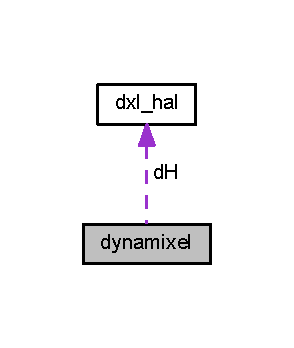
\includegraphics[width=141pt]{d5/d16/a00029}
\end{center}
\end{figure}
\subsection*{Public Member Functions}
\begin{DoxyCompactItemize}
\item 
\hyperlink{a00004_a7aa668a213db6a41bede8e08a6fec830}{dynamixel} ()
\begin{DoxyCompactList}\small\item\em Default constructor. \end{DoxyCompactList}\item 
\hyperlink{a00004_a5d4fed957a4b2d1690c0fa72127f5cbf}{dynamixel} (Q\+String port\+\_\+num, int baud\+\_\+rate=1000000)
\begin{DoxyCompactList}\small\item\em Initialization constructor. \end{DoxyCompactList}\item 
bool \hyperlink{a00004_a5ae4b2c6eb4c91f404f973ee8e6a1914}{is\+Open} ()
\begin{DoxyCompactList}\small\item\em True if the port is open. \end{DoxyCompactList}\item 
int \hyperlink{a00004_a87960244d5846ae7583e37d2407eb61e}{initialize} (Q\+String port\+\_\+num, int baud\+\_\+rate)
\begin{DoxyCompactList}\small\item\em Initializates the port. \end{DoxyCompactList}\item 
int \hyperlink{a00004_a7554c7889896e29e11a62027d89f3fdf}{change\+\_\+baudrate} (int baud\+\_\+rate)
\begin{DoxyCompactList}\small\item\em Changes the current baud rate. \end{DoxyCompactList}\item 
int \hyperlink{a00004_a92ea074ed1c1a9cf29e039f8c425f01a}{terminate} (void)
\begin{DoxyCompactList}\small\item\em Closes the comunication. \end{DoxyCompactList}\item 
int \hyperlink{a00004_ac8440d5d34ae3c4618b28fdbbd748edc}{get\+\_\+comm\+\_\+result} ()
\begin{DoxyCompactList}\small\item\em Returns the current com status. \end{DoxyCompactList}\item 
void \hyperlink{a00004_a479187cd8940c16dd4374eb5be22b888}{tx\+\_\+packet} (void)
\begin{DoxyCompactList}\small\item\em Sends a packet. \end{DoxyCompactList}\item 
void \hyperlink{a00004_aa26d2d2dff768563a1cb1480aa061608}{rx\+\_\+packet} (void)
\begin{DoxyCompactList}\small\item\em Receives a packet. \end{DoxyCompactList}\item 
void \hyperlink{a00004_aebfc569c6b1eb0b98f8c385f0f921fc0}{txrx\+\_\+packet} (void)
\begin{DoxyCompactList}\small\item\em Sends and receives a packet. \end{DoxyCompactList}\item 
void \hyperlink{a00004_a84e24c72c3e5be866f8b28c2e5bd1d95}{set\+\_\+txpacket\+\_\+id} (int id)
\begin{DoxyCompactList}\small\item\em Sets the sending packet I\+D. \end{DoxyCompactList}\item 
void \hyperlink{a00004_a209a43f983f214323b6f0a627d5e8c13}{set\+\_\+txpacket\+\_\+instruction} (int instruction)
\begin{DoxyCompactList}\small\item\em Sets the sending packet instruction. \end{DoxyCompactList}\item 
void \hyperlink{a00004_a2c3d31bbbed70a69918e9972a620384b}{set\+\_\+txpacket\+\_\+parameter} (int index, int value)
\begin{DoxyCompactList}\small\item\em Sets the sending packet parameter. \end{DoxyCompactList}\item 
void \hyperlink{a00004_a829278f48e21c810b172eb8cab3b86de}{set\+\_\+txpacket\+\_\+length} (int length)
\begin{DoxyCompactList}\small\item\em Sets the sending packet length. \end{DoxyCompactList}\item 
bool \hyperlink{a00004_a843b0aac721e4264e7e3097f80980243}{get\+\_\+rxpacket\+\_\+error} (int error)
\begin{DoxyCompactList}\small\item\em Returns false if no receive error and true if there\textquotesingle{}s an error. \end{DoxyCompactList}\item 
int \hyperlink{a00004_a6e62341ef9f51b6e152e769bd7be9d75}{get\+\_\+rxpacket\+\_\+error\+\_\+byte} (void)
\begin{DoxyCompactList}\small\item\em Returns the error byte. \end{DoxyCompactList}\item 
int \hyperlink{a00004_a68b5fa99719a9aec0734ecfb0635503b}{get\+\_\+rxpacket\+\_\+parameter} (int index)
\begin{DoxyCompactList}\small\item\em Returns the received parameter. \end{DoxyCompactList}\item 
int \hyperlink{a00004_ae9cc18fdeda8329f68fa0f2f0a7a9aba}{get\+\_\+rxpacket\+\_\+length} ()
\begin{DoxyCompactList}\small\item\em Returns the received packet length. \end{DoxyCompactList}\item 
void \hyperlink{a00004_af2bd714423e7c4fc089762805c0c71f3}{ping} (int id)
\begin{DoxyCompactList}\small\item\em Ping to the selected id, check com status for the ping result. \end{DoxyCompactList}\item 
int \hyperlink{a00004_a888404b41c4c4395a0b745c77ff2cea9}{read\+\_\+byte} (int id, int address)
\begin{DoxyCompactList}\small\item\em Reads a byte from the selected I\+D at the selected address. \end{DoxyCompactList}\item 
void \hyperlink{a00004_a66c1e32cc45dd46d329f1fc212e46a3d}{write\+\_\+byte} (int id, int address, int value)
\begin{DoxyCompactList}\small\item\em Writes a byte to the selected I\+D at the selected address. \end{DoxyCompactList}\item 
int \hyperlink{a00004_a45e99341e82c5114f6e829c9141bf96f}{read\+\_\+word} (int id, int address)
\begin{DoxyCompactList}\small\item\em Reads a word to the selected I\+D at the selected address. \end{DoxyCompactList}\item 
void \hyperlink{a00004_a925f62ce5e261e5ef4fe6dc46bdc7c63}{write\+\_\+word} (int id, int address, int value)
\begin{DoxyCompactList}\small\item\em Writes a word to the selected I\+D at the selected address. \end{DoxyCompactList}\item 
double \hyperlink{a00004_a2fa5375537184c279a9ebfcfc0425071}{get\+\_\+packet\+\_\+time} ()
\begin{DoxyCompactList}\small\item\em Returns the packet time. \end{DoxyCompactList}\item 
void \hyperlink{a00004_a067f82c21ed176e18fa224d16f3d1c5b}{set\+\_\+packet\+\_\+timeout} (int Num\+Rcv\+Byte)
\begin{DoxyCompactList}\small\item\em Sets the timeout in number of received bytes. \end{DoxyCompactList}\item 
void \hyperlink{a00004_a125b42f776c4aac520f274074f68b591}{set\+\_\+packet\+\_\+timeout\+\_\+ms} (int msec)
\begin{DoxyCompactList}\small\item\em Sets the timeout in ms. \end{DoxyCompactList}\item 
bool \hyperlink{a00004_a00d08481ebc4dee19debecf43f888522}{is\+\_\+packet\+\_\+timeout} ()
\begin{DoxyCompactList}\small\item\em Returns true if the packet is timeout. \end{DoxyCompactList}\end{DoxyCompactItemize}
\subsection*{Private Attributes}
\begin{DoxyCompactItemize}
\item 
\hyperlink{a00003}{dxl\+\_\+hal} \hyperlink{a00004_ae003cc90ada6d7b70eaa4ea9d42d4deb}{d\+H}
\begin{DoxyCompactList}\small\item\em Conains the serial port comunication. \end{DoxyCompactList}\item 
unsigned char \hyperlink{a00004_afd94dcf01b8e96298727776e222de722}{gb\+Instruction\+Packet} \mbox{[}M\+A\+X\+N\+U\+M\+\_\+\+T\+X\+P\+A\+C\+K\+E\+T\mbox{]} = \{0\}
\begin{DoxyCompactList}\small\item\em Contains all the instructions. \end{DoxyCompactList}\item 
unsigned char \hyperlink{a00004_aa57c86d3bbbeaf5c9d4f6bd00376b04f}{gb\+Status\+Packet} \mbox{[}M\+A\+X\+N\+U\+M\+\_\+\+R\+X\+P\+A\+C\+K\+E\+T\mbox{]} = \{0\}
\begin{DoxyCompactList}\small\item\em Contains the status. \end{DoxyCompactList}\item 
unsigned int \hyperlink{a00004_a333686e1b5903d16c41df8172b6bd5a8}{gb\+Rx\+Packet\+Length} = 0
\begin{DoxyCompactList}\small\item\em Received packet length. \end{DoxyCompactList}\item 
unsigned int \hyperlink{a00004_a9d590ce24791d111c2db9b66be1e046d}{gb\+Rx\+Get\+Length} = 0
\begin{DoxyCompactList}\small\item\em Temporal length from the received packet. \end{DoxyCompactList}\item 
double \hyperlink{a00004_a6c6314fb7070e6fd361e57c5de17e0ec}{gd\+Packet\+Start\+Time} = 0.\+0
\begin{DoxyCompactList}\small\item\em Packet start time. \end{DoxyCompactList}\item 
double \hyperlink{a00004_a2173f25c6299da7ddb37ba3d2bf1f738}{gd\+Byte\+Trans\+Time} = 0.\+0
\begin{DoxyCompactList}\small\item\em Byte transmission time. \end{DoxyCompactList}\item 
double \hyperlink{a00004_a9f47887864517d74955a2bc787ae4456}{gd\+Rcv\+Wait\+Time} = 0.\+0
\begin{DoxyCompactList}\small\item\em Receive wait time. \end{DoxyCompactList}\item 
int \hyperlink{a00004_a5b603f6bed7ccc595f1f50bd6a6ebbfc}{gb\+Comm\+Status} = C\+O\+M\+M\+\_\+\+R\+X\+S\+U\+C\+C\+E\+S\+S
\begin{DoxyCompactList}\small\item\em Current communication status. \end{DoxyCompactList}\item 
int \hyperlink{a00004_ad10e0e49f5fef04bf789a89c14cc470a}{gi\+Bus\+Using} = 0
\begin{DoxyCompactList}\small\item\em True if the bus if being used. \end{DoxyCompactList}\end{DoxyCompactItemize}


\subsection{Detailed Description}
Dynamixel 1.\+0 protocol class. 

\subsection{Constructor \& Destructor Documentation}
\hypertarget{a00004_a7aa668a213db6a41bede8e08a6fec830}{}\index{dynamixel@{dynamixel}!dynamixel@{dynamixel}}
\index{dynamixel@{dynamixel}!dynamixel@{dynamixel}}
\subsubsection[{dynamixel}]{\setlength{\rightskip}{0pt plus 5cm}dynamixel\+::dynamixel (
\begin{DoxyParamCaption}
{}
\end{DoxyParamCaption}
)\hspace{0.3cm}{\ttfamily [inline]}}\label{a00004_a7aa668a213db6a41bede8e08a6fec830}


Default constructor. 


\begin{DoxyCode}
00097 \{\}
\end{DoxyCode}
\hypertarget{a00004_a5d4fed957a4b2d1690c0fa72127f5cbf}{}\index{dynamixel@{dynamixel}!dynamixel@{dynamixel}}
\index{dynamixel@{dynamixel}!dynamixel@{dynamixel}}
\subsubsection[{dynamixel}]{\setlength{\rightskip}{0pt plus 5cm}dynamixel\+::dynamixel (
\begin{DoxyParamCaption}
\item[{Q\+String}]{port\+\_\+num, }
\item[{int}]{baud\+\_\+rate = {\ttfamily 1000000}}
\end{DoxyParamCaption}
)}\label{a00004_a5d4fed957a4b2d1690c0fa72127f5cbf}


Initialization constructor. 


\begin{DoxyCode}
00011 \{
00012     \hyperlink{a00004_a87960244d5846ae7583e37d2407eb61e}{initialize}(port\_num, baud\_rate);
00013 \}
\end{DoxyCode}


\subsection{Member Function Documentation}
\hypertarget{a00004_a7554c7889896e29e11a62027d89f3fdf}{}\index{dynamixel@{dynamixel}!change\+\_\+baudrate@{change\+\_\+baudrate}}
\index{change\+\_\+baudrate@{change\+\_\+baudrate}!dynamixel@{dynamixel}}
\subsubsection[{change\+\_\+baudrate}]{\setlength{\rightskip}{0pt plus 5cm}int dynamixel\+::change\+\_\+baudrate (
\begin{DoxyParamCaption}
\item[{int}]{baud\+\_\+rate}
\end{DoxyParamCaption}
)}\label{a00004_a7554c7889896e29e11a62027d89f3fdf}


Changes the current baud rate. 


\begin{DoxyCode}
00031 \{
00032     \textcolor{keywordtype}{int} result = 0;
00033     \textcolor{keywordtype}{float} baudrate = (float)baud\_rate;
00034     
00035     result = \hyperlink{a00004_ae003cc90ada6d7b70eaa4ea9d42d4deb}{dH}.\hyperlink{a00003_a0eaaa5340bc9dce73cc920dc8befe5b0}{change\_baudrate}(baudrate);
00036     \textcolor{keywordflow}{if}(result == 1)
00037         \hyperlink{a00004_a2173f25c6299da7ddb37ba3d2bf1f738}{gdByteTransTime} = 1000.0f / baudrate * 10.0; \textcolor{comment}{// 1000/baudrate(bit per msec) *
       10(start bit + data bit + stop bit)}
00038 
00039     \textcolor{keywordflow}{return} result;
00040 \}
\end{DoxyCode}
\hypertarget{a00004_ac8440d5d34ae3c4618b28fdbbd748edc}{}\index{dynamixel@{dynamixel}!get\+\_\+comm\+\_\+result@{get\+\_\+comm\+\_\+result}}
\index{get\+\_\+comm\+\_\+result@{get\+\_\+comm\+\_\+result}!dynamixel@{dynamixel}}
\subsubsection[{get\+\_\+comm\+\_\+result}]{\setlength{\rightskip}{0pt plus 5cm}int dynamixel\+::get\+\_\+comm\+\_\+result (
\begin{DoxyParamCaption}
{}
\end{DoxyParamCaption}
)\hspace{0.3cm}{\ttfamily [inline]}}\label{a00004_ac8440d5d34ae3c4618b28fdbbd748edc}


Returns the current com status. 


\begin{DoxyCode}
00115 \{ \textcolor{keywordflow}{return} \hyperlink{a00004_a5b603f6bed7ccc595f1f50bd6a6ebbfc}{gbCommStatus}; \}
\end{DoxyCode}
\hypertarget{a00004_a2fa5375537184c279a9ebfcfc0425071}{}\index{dynamixel@{dynamixel}!get\+\_\+packet\+\_\+time@{get\+\_\+packet\+\_\+time}}
\index{get\+\_\+packet\+\_\+time@{get\+\_\+packet\+\_\+time}!dynamixel@{dynamixel}}
\subsubsection[{get\+\_\+packet\+\_\+time}]{\setlength{\rightskip}{0pt plus 5cm}double dynamixel\+::get\+\_\+packet\+\_\+time (
\begin{DoxyParamCaption}
\item[{void}]{}
\end{DoxyParamCaption}
)}\label{a00004_a2fa5375537184c279a9ebfcfc0425071}


Returns the packet time. 


\begin{DoxyCode}
00050 \{
00051     \textcolor{keywordtype}{double} elapsed\_time;
00052 
00053     elapsed\_time = (double)(\hyperlink{a00004_ae003cc90ada6d7b70eaa4ea9d42d4deb}{dH}.\hyperlink{a00003_a6b6b7381c45308662fc3df6e7f74bc61}{get\_curr\_time}() - 
      \hyperlink{a00004_a6c6314fb7070e6fd361e57c5de17e0ec}{gdPacketStartTime});
00054 
00055     \textcolor{comment}{// Overflow}
00056     \textcolor{keywordflow}{if}(elapsed\_time < 0) \hyperlink{a00004_a6c6314fb7070e6fd361e57c5de17e0ec}{gdPacketStartTime} = \hyperlink{a00004_ae003cc90ada6d7b70eaa4ea9d42d4deb}{dH}.\hyperlink{a00003_a6b6b7381c45308662fc3df6e7f74bc61}{get\_curr\_time}();
00057     
00058     \textcolor{keywordflow}{return} elapsed\_time;
00059 \}
\end{DoxyCode}
\hypertarget{a00004_a843b0aac721e4264e7e3097f80980243}{}\index{dynamixel@{dynamixel}!get\+\_\+rxpacket\+\_\+error@{get\+\_\+rxpacket\+\_\+error}}
\index{get\+\_\+rxpacket\+\_\+error@{get\+\_\+rxpacket\+\_\+error}!dynamixel@{dynamixel}}
\subsubsection[{get\+\_\+rxpacket\+\_\+error}]{\setlength{\rightskip}{0pt plus 5cm}bool dynamixel\+::get\+\_\+rxpacket\+\_\+error (
\begin{DoxyParamCaption}
\item[{int}]{error}
\end{DoxyParamCaption}
)}\label{a00004_a843b0aac721e4264e7e3097f80980243}


Returns false if no receive error and true if there\textquotesingle{}s an error. 


\begin{DoxyParams}{Parameters}
{\em error} & Selects the error to check \\
\hline
\end{DoxyParams}

\begin{DoxyCode}
00271 \{
00272     \textcolor{keywordflow}{if}( \hyperlink{a00004_aa57c86d3bbbeaf5c9d4f6bd00376b04f}{gbStatusPacket}[PRT1\_PKT\_ERRBIT] & (\textcolor{keywordtype}{unsigned} \textcolor{keywordtype}{char})error )
00273         \textcolor{keywordflow}{return} \textcolor{keyword}{true};
00274 
00275     \textcolor{keywordflow}{return} \textcolor{keyword}{false};
00276 \}
\end{DoxyCode}
\hypertarget{a00004_a6e62341ef9f51b6e152e769bd7be9d75}{}\index{dynamixel@{dynamixel}!get\+\_\+rxpacket\+\_\+error\+\_\+byte@{get\+\_\+rxpacket\+\_\+error\+\_\+byte}}
\index{get\+\_\+rxpacket\+\_\+error\+\_\+byte@{get\+\_\+rxpacket\+\_\+error\+\_\+byte}!dynamixel@{dynamixel}}
\subsubsection[{get\+\_\+rxpacket\+\_\+error\+\_\+byte}]{\setlength{\rightskip}{0pt plus 5cm}int dynamixel\+::get\+\_\+rxpacket\+\_\+error\+\_\+byte (
\begin{DoxyParamCaption}
\item[{void}]{}
\end{DoxyParamCaption}
)}\label{a00004_a6e62341ef9f51b6e152e769bd7be9d75}


Returns the error byte. 


\begin{DoxyCode}
00279 \{
00280     \textcolor{keywordflow}{return} \hyperlink{a00004_aa57c86d3bbbeaf5c9d4f6bd00376b04f}{gbStatusPacket}[PRT1\_PKT\_ERRBIT];
00281 \}
\end{DoxyCode}
\hypertarget{a00004_ae9cc18fdeda8329f68fa0f2f0a7a9aba}{}\index{dynamixel@{dynamixel}!get\+\_\+rxpacket\+\_\+length@{get\+\_\+rxpacket\+\_\+length}}
\index{get\+\_\+rxpacket\+\_\+length@{get\+\_\+rxpacket\+\_\+length}!dynamixel@{dynamixel}}
\subsubsection[{get\+\_\+rxpacket\+\_\+length}]{\setlength{\rightskip}{0pt plus 5cm}int dynamixel\+::get\+\_\+rxpacket\+\_\+length (
\begin{DoxyParamCaption}
{}
\end{DoxyParamCaption}
)}\label{a00004_ae9cc18fdeda8329f68fa0f2f0a7a9aba}


Returns the received packet length. 


\begin{DoxyCode}
00289 \{
00290     \textcolor{keywordflow}{return} (\textcolor{keywordtype}{int})\hyperlink{a00004_aa57c86d3bbbeaf5c9d4f6bd00376b04f}{gbStatusPacket}[PRT1\_PKT\_LENGTH];
00291 \}
\end{DoxyCode}
\hypertarget{a00004_a68b5fa99719a9aec0734ecfb0635503b}{}\index{dynamixel@{dynamixel}!get\+\_\+rxpacket\+\_\+parameter@{get\+\_\+rxpacket\+\_\+parameter}}
\index{get\+\_\+rxpacket\+\_\+parameter@{get\+\_\+rxpacket\+\_\+parameter}!dynamixel@{dynamixel}}
\subsubsection[{get\+\_\+rxpacket\+\_\+parameter}]{\setlength{\rightskip}{0pt plus 5cm}int dynamixel\+::get\+\_\+rxpacket\+\_\+parameter (
\begin{DoxyParamCaption}
\item[{int}]{index}
\end{DoxyParamCaption}
)}\label{a00004_a68b5fa99719a9aec0734ecfb0635503b}


Returns the received parameter. 


\begin{DoxyCode}
00284 \{
00285     \textcolor{keywordflow}{return} (\textcolor{keywordtype}{int})\hyperlink{a00004_aa57c86d3bbbeaf5c9d4f6bd00376b04f}{gbStatusPacket}[PRT1\_PKT\_PARAMETER0+index];
00286 \}
\end{DoxyCode}
\hypertarget{a00004_a87960244d5846ae7583e37d2407eb61e}{}\index{dynamixel@{dynamixel}!initialize@{initialize}}
\index{initialize@{initialize}!dynamixel@{dynamixel}}
\subsubsection[{initialize}]{\setlength{\rightskip}{0pt plus 5cm}int dynamixel\+::initialize (
\begin{DoxyParamCaption}
\item[{Q\+String}]{port\+\_\+num, }
\item[{int}]{baud\+\_\+rate}
\end{DoxyParamCaption}
)}\label{a00004_a87960244d5846ae7583e37d2407eb61e}


Initializates the port. 


\begin{DoxyCode}
00016 \{
00017     \textcolor{keywordflow}{if}( baud\_rate < 1900 ) \textcolor{keywordflow}{return} 0;
00018 
00019     \textcolor{keywordflow}{if}( not \hyperlink{a00004_ae003cc90ada6d7b70eaa4ea9d42d4deb}{dH}.\hyperlink{a00003_ab631c2a5533125f14db9a8ec1c33aa7c}{open}(port\_num, baud\_rate) ) \textcolor{keywordflow}{return} \textcolor{keyword}{false};
00020     
00021     \textcolor{comment}{// 1000/baudrate(bit per msec) * 10(start bit + data bit + stop bit)}
00022     \hyperlink{a00004_a2173f25c6299da7ddb37ba3d2bf1f738}{gdByteTransTime} = 1000.0 / (double)baud\_rate * 10.0; 
00023 
00024     \hyperlink{a00004_a5b603f6bed7ccc595f1f50bd6a6ebbfc}{gbCommStatus} = COMM\_RXSUCCESS;
00025     \hyperlink{a00004_ad10e0e49f5fef04bf789a89c14cc470a}{giBusUsing} = 0;
00026 
00027     \textcolor{keywordflow}{return} \textcolor{keyword}{true};
00028 \}
\end{DoxyCode}
\hypertarget{a00004_a00d08481ebc4dee19debecf43f888522}{}\index{dynamixel@{dynamixel}!is\+\_\+packet\+\_\+timeout@{is\+\_\+packet\+\_\+timeout}}
\index{is\+\_\+packet\+\_\+timeout@{is\+\_\+packet\+\_\+timeout}!dynamixel@{dynamixel}}
\subsubsection[{is\+\_\+packet\+\_\+timeout}]{\setlength{\rightskip}{0pt plus 5cm}bool dynamixel\+::is\+\_\+packet\+\_\+timeout (
\begin{DoxyParamCaption}
\item[{void}]{}
\end{DoxyParamCaption}
)}\label{a00004_a00d08481ebc4dee19debecf43f888522}


Returns true if the packet is timeout. 

\begin{DoxyReturn}{Returns}
True if the packet is timeout 
\end{DoxyReturn}

\begin{DoxyCode}
00074 \{
00075     \textcolor{keywordflow}{if}(this->\hyperlink{a00004_a2fa5375537184c279a9ebfcfc0425071}{get\_packet\_time}() > \hyperlink{a00004_a9f47887864517d74955a2bc787ae4456}{gdRcvWaitTime})
00076         \textcolor{keywordflow}{return} \textcolor{keyword}{true};
00077     \textcolor{keywordflow}{return} \textcolor{keyword}{false};
00078 \}
\end{DoxyCode}
\hypertarget{a00004_a5ae4b2c6eb4c91f404f973ee8e6a1914}{}\index{dynamixel@{dynamixel}!is\+Open@{is\+Open}}
\index{is\+Open@{is\+Open}!dynamixel@{dynamixel}}
\subsubsection[{is\+Open}]{\setlength{\rightskip}{0pt plus 5cm}bool dynamixel\+::is\+Open (
\begin{DoxyParamCaption}
{}
\end{DoxyParamCaption}
)\hspace{0.3cm}{\ttfamily [inline]}}\label{a00004_a5ae4b2c6eb4c91f404f973ee8e6a1914}


True if the port is open. 


\begin{DoxyCode}
00103 \{ \textcolor{keywordflow}{return} \hyperlink{a00004_ae003cc90ada6d7b70eaa4ea9d42d4deb}{dH}.\hyperlink{a00003_a88bba601b5c9f285fcdc14e18a1f3398}{isOpen}(); \}
\end{DoxyCode}
\hypertarget{a00004_af2bd714423e7c4fc089762805c0c71f3}{}\index{dynamixel@{dynamixel}!ping@{ping}}
\index{ping@{ping}!dynamixel@{dynamixel}}
\subsubsection[{ping}]{\setlength{\rightskip}{0pt plus 5cm}void dynamixel\+::ping (
\begin{DoxyParamCaption}
\item[{int}]{id}
\end{DoxyParamCaption}
)}\label{a00004_af2bd714423e7c4fc089762805c0c71f3}


Ping to the selected id, check com status for the ping result. 


\begin{DoxyParams}{Parameters}
{\em id} & I\+D where the ping is done \\
\hline
\end{DoxyParams}

\begin{DoxyCode}
00294 \{
00295     \textcolor{keywordflow}{while}(\hyperlink{a00004_ad10e0e49f5fef04bf789a89c14cc470a}{giBusUsing});
00296 
00297     \hyperlink{a00004_afd94dcf01b8e96298727776e222de722}{gbInstructionPacket}[PRT1\_PKT\_ID] = (\textcolor{keywordtype}{unsigned} char)\textcolor{keywordtype}{id};
00298     \hyperlink{a00004_afd94dcf01b8e96298727776e222de722}{gbInstructionPacket}[PRT1\_PKT\_INSTRUCTION] = INST\_PING;
00299     \hyperlink{a00004_afd94dcf01b8e96298727776e222de722}{gbInstructionPacket}[PRT1\_PKT\_LENGTH] = 2;
00300     
00301     \hyperlink{a00004_aebfc569c6b1eb0b98f8c385f0f921fc0}{txrx\_packet}();
00302 \}
\end{DoxyCode}
\hypertarget{a00004_a888404b41c4c4395a0b745c77ff2cea9}{}\index{dynamixel@{dynamixel}!read\+\_\+byte@{read\+\_\+byte}}
\index{read\+\_\+byte@{read\+\_\+byte}!dynamixel@{dynamixel}}
\subsubsection[{read\+\_\+byte}]{\setlength{\rightskip}{0pt plus 5cm}int dynamixel\+::read\+\_\+byte (
\begin{DoxyParamCaption}
\item[{int}]{id, }
\item[{int}]{address}
\end{DoxyParamCaption}
)}\label{a00004_a888404b41c4c4395a0b745c77ff2cea9}


Reads a byte from the selected I\+D at the selected address. 


\begin{DoxyParams}{Parameters}
{\em id} & Selects the I\+D to read the byte \\
\hline
{\em address} & Selects the address to read the byte \\
\hline
\end{DoxyParams}

\begin{DoxyCode}
00305 \{
00306     \textcolor{keywordflow}{while}(\hyperlink{a00004_ad10e0e49f5fef04bf789a89c14cc470a}{giBusUsing});
00307 
00308     \hyperlink{a00004_afd94dcf01b8e96298727776e222de722}{gbInstructionPacket}[PRT1\_PKT\_ID] = (\textcolor{keywordtype}{unsigned} char)\textcolor{keywordtype}{id};
00309     \hyperlink{a00004_afd94dcf01b8e96298727776e222de722}{gbInstructionPacket}[PRT1\_PKT\_INSTRUCTION] = INST\_READ;
00310     \hyperlink{a00004_afd94dcf01b8e96298727776e222de722}{gbInstructionPacket}[PRT1\_PKT\_PARAMETER0+0] = (\textcolor{keywordtype}{unsigned} char)address;
00311     \hyperlink{a00004_afd94dcf01b8e96298727776e222de722}{gbInstructionPacket}[PRT1\_PKT\_PARAMETER0+1] = 1;
00312     \hyperlink{a00004_afd94dcf01b8e96298727776e222de722}{gbInstructionPacket}[PRT1\_PKT\_LENGTH] = 4;
00313     
00314     \hyperlink{a00004_aebfc569c6b1eb0b98f8c385f0f921fc0}{txrx\_packet}();
00315 
00316     \textcolor{keywordflow}{return} (\textcolor{keywordtype}{int})\hyperlink{a00004_aa57c86d3bbbeaf5c9d4f6bd00376b04f}{gbStatusPacket}[PRT1\_PKT\_PARAMETER0];
00317 \}
\end{DoxyCode}
\hypertarget{a00004_a45e99341e82c5114f6e829c9141bf96f}{}\index{dynamixel@{dynamixel}!read\+\_\+word@{read\+\_\+word}}
\index{read\+\_\+word@{read\+\_\+word}!dynamixel@{dynamixel}}
\subsubsection[{read\+\_\+word}]{\setlength{\rightskip}{0pt plus 5cm}int dynamixel\+::read\+\_\+word (
\begin{DoxyParamCaption}
\item[{int}]{id, }
\item[{int}]{address}
\end{DoxyParamCaption}
)}\label{a00004_a45e99341e82c5114f6e829c9141bf96f}


Reads a word to the selected I\+D at the selected address. 


\begin{DoxyParams}{Parameters}
{\em id} & Selects the I\+D to read the word \\
\hline
{\em address} & Selects the address to read the word \\
\hline
\end{DoxyParams}

\begin{DoxyCode}
00333 \{
00334     \textcolor{keywordflow}{while}(\hyperlink{a00004_ad10e0e49f5fef04bf789a89c14cc470a}{giBusUsing});
00335 
00336     \hyperlink{a00004_afd94dcf01b8e96298727776e222de722}{gbInstructionPacket}[PRT1\_PKT\_ID] = (\textcolor{keywordtype}{unsigned} char)\textcolor{keywordtype}{id};
00337     \hyperlink{a00004_afd94dcf01b8e96298727776e222de722}{gbInstructionPacket}[PRT1\_PKT\_INSTRUCTION] = INST\_READ;
00338     \hyperlink{a00004_afd94dcf01b8e96298727776e222de722}{gbInstructionPacket}[PRT1\_PKT\_PARAMETER0+0] = (\textcolor{keywordtype}{unsigned} char)address;
00339     \hyperlink{a00004_afd94dcf01b8e96298727776e222de722}{gbInstructionPacket}[PRT1\_PKT\_PARAMETER0+1] = 2;
00340     \hyperlink{a00004_afd94dcf01b8e96298727776e222de722}{gbInstructionPacket}[PRT1\_PKT\_LENGTH] = 4;
00341     
00342     \hyperlink{a00004_aebfc569c6b1eb0b98f8c385f0f921fc0}{txrx\_packet}();
00343 
00344     \textcolor{keywordflow}{return} MAKEWORD((\textcolor{keywordtype}{int})\hyperlink{a00004_aa57c86d3bbbeaf5c9d4f6bd00376b04f}{gbStatusPacket}[PRT1\_PKT\_PARAMETER0+0], (\textcolor{keywordtype}{int})
      \hyperlink{a00004_aa57c86d3bbbeaf5c9d4f6bd00376b04f}{gbStatusPacket}[PRT1\_PKT\_PARAMETER0+1]);
00345 \}
\end{DoxyCode}
\hypertarget{a00004_aa26d2d2dff768563a1cb1480aa061608}{}\index{dynamixel@{dynamixel}!rx\+\_\+packet@{rx\+\_\+packet}}
\index{rx\+\_\+packet@{rx\+\_\+packet}!dynamixel@{dynamixel}}
\subsubsection[{rx\+\_\+packet}]{\setlength{\rightskip}{0pt plus 5cm}void dynamixel\+::rx\+\_\+packet (
\begin{DoxyParamCaption}
\item[{void}]{}
\end{DoxyParamCaption}
)}\label{a00004_aa26d2d2dff768563a1cb1480aa061608}


Receives a packet. 


\begin{DoxyCode}
00144 \{
00145     \textcolor{keywordtype}{unsigned} \textcolor{keywordtype}{char} i = 0, j = 0, nRead = 0;
00146     \textcolor{keywordtype}{unsigned} \textcolor{keywordtype}{char} checksum = 0;
00147 
00148     \textcolor{keywordflow}{if}( \hyperlink{a00004_ad10e0e49f5fef04bf789a89c14cc470a}{giBusUsing} == 0 )
00149         \textcolor{keywordflow}{return};
00150 
00151     \textcolor{keywordflow}{if}( \hyperlink{a00004_afd94dcf01b8e96298727776e222de722}{gbInstructionPacket}[PRT1\_PKT\_ID] == BROADCAST\_ID )
00152     \{
00153         \hyperlink{a00004_a5b603f6bed7ccc595f1f50bd6a6ebbfc}{gbCommStatus} = COMM\_RXSUCCESS;
00154         \hyperlink{a00004_ad10e0e49f5fef04bf789a89c14cc470a}{giBusUsing} = 0;
00155         \textcolor{keywordflow}{return};
00156     \}
00157     
00158     \textcolor{keywordflow}{if}( \hyperlink{a00004_a5b603f6bed7ccc595f1f50bd6a6ebbfc}{gbCommStatus} == COMM\_TXSUCCESS )
00159     \{
00160         \hyperlink{a00004_a9d590ce24791d111c2db9b66be1e046d}{gbRxGetLength} = 0;
00161         \textcolor{comment}{//gbRxPacketLength = 6; //minimum wait length}
00162     \}
00163     
00164     \textcolor{keywordflow}{while}(1)
00165     \{
00166         nRead = \hyperlink{a00004_ae003cc90ada6d7b70eaa4ea9d42d4deb}{dH}.\hyperlink{a00003_ac36331febb2eaa66303af3483795742a}{read}( &\hyperlink{a00004_aa57c86d3bbbeaf5c9d4f6bd00376b04f}{gbStatusPacket}[\hyperlink{a00004_a9d590ce24791d111c2db9b66be1e046d}{gbRxGetLength}], 
      \hyperlink{a00004_a333686e1b5903d16c41df8172b6bd5a8}{gbRxPacketLength} - gbRxGetLength );
00167         gbRxGetLength += nRead;
00168 
00169         \textcolor{keywordflow}{if}(gbRxGetLength > 4)
00170             \hyperlink{a00004_a333686e1b5903d16c41df8172b6bd5a8}{gbRxPacketLength} = \hyperlink{a00004_aa57c86d3bbbeaf5c9d4f6bd00376b04f}{gbStatusPacket}[PRT1\_PKT\_LENGTH] + 4;
00171 
00172         \textcolor{keywordflow}{if}( gbRxGetLength < \hyperlink{a00004_a333686e1b5903d16c41df8172b6bd5a8}{gbRxPacketLength} )
00173         \{
00174             \textcolor{keywordflow}{if}( \hyperlink{a00004_a00d08481ebc4dee19debecf43f888522}{is\_packet\_timeout}() == 1 )
00175             \{
00176                 \textcolor{keywordflow}{if}(gbRxGetLength == 0)
00177                     \hyperlink{a00004_a5b603f6bed7ccc595f1f50bd6a6ebbfc}{gbCommStatus} = COMM\_RXTIMEOUT;
00178                 \textcolor{keywordflow}{else}
00179                     \hyperlink{a00004_a5b603f6bed7ccc595f1f50bd6a6ebbfc}{gbCommStatus} = COMM\_RXCORRUPT;
00180                 \hyperlink{a00004_ad10e0e49f5fef04bf789a89c14cc470a}{giBusUsing} = 0;
00181                 \textcolor{keywordflow}{return};
00182             \}
00183             \hyperlink{a00004_a5b603f6bed7ccc595f1f50bd6a6ebbfc}{gbCommStatus} = COMM\_RXWAITING;
00184             \textcolor{comment}{//return;           }
00185         \}
00186         \textcolor{keywordflow}{else}
00187         \{
00188             \textcolor{keywordflow}{break};
00189         \}
00190     \}
00191 
00192     \textcolor{comment}{// Find packet header}
00193     \textcolor{keywordflow}{for}( i=0; i<(gbRxGetLength-1); i++ )
00194     \{
00195         \textcolor{keywordflow}{if}( \hyperlink{a00004_aa57c86d3bbbeaf5c9d4f6bd00376b04f}{gbStatusPacket}[i] == 0xff && \hyperlink{a00004_aa57c86d3bbbeaf5c9d4f6bd00376b04f}{gbStatusPacket}[i+1] == 0xff )
00196             \textcolor{keywordflow}{break};
00197         \textcolor{keywordflow}{else} \textcolor{keywordflow}{if}( i == gbRxGetLength-2 && \hyperlink{a00004_aa57c86d3bbbeaf5c9d4f6bd00376b04f}{gbStatusPacket}[gbRxGetLength-1] == 0xff )
00198             \textcolor{keywordflow}{break};
00199         \textcolor{keywordflow}{else} \{
00200             \hyperlink{a00004_a5b603f6bed7ccc595f1f50bd6a6ebbfc}{gbCommStatus} = COMM\_RXCORRUPT;
00201             \textcolor{keywordflow}{return};
00202         \}
00203     \}
00204 
00205     \textcolor{keywordflow}{if}( i > 0 )
00206     \{
00207         \textcolor{keywordflow}{for}( j=0; j<(gbRxGetLength-i); j++ )
00208             \hyperlink{a00004_aa57c86d3bbbeaf5c9d4f6bd00376b04f}{gbStatusPacket}[j] = \hyperlink{a00004_aa57c86d3bbbeaf5c9d4f6bd00376b04f}{gbStatusPacket}[j + i];
00209             
00210         gbRxGetLength -= i;     
00211     \}
00212 
00213     \textcolor{comment}{// Check id pairing}
00214     \textcolor{keywordflow}{if}( \hyperlink{a00004_afd94dcf01b8e96298727776e222de722}{gbInstructionPacket}[PRT1\_PKT\_ID] != \hyperlink{a00004_aa57c86d3bbbeaf5c9d4f6bd00376b04f}{gbStatusPacket}[PRT1\_PKT\_ID])
00215     \{
00216         \hyperlink{a00004_a5b603f6bed7ccc595f1f50bd6a6ebbfc}{gbCommStatus} = COMM\_RXCORRUPT;
00217         \hyperlink{a00004_ad10e0e49f5fef04bf789a89c14cc470a}{giBusUsing} = 0;
00218         \textcolor{keywordflow}{return};
00219     \}
00220     
00221     \textcolor{comment}{// Check checksum}
00222     \textcolor{keywordflow}{for}( i=0; i<(\hyperlink{a00004_aa57c86d3bbbeaf5c9d4f6bd00376b04f}{gbStatusPacket}[PRT1\_PKT\_LENGTH]+1); i++ )
00223         checksum += \hyperlink{a00004_aa57c86d3bbbeaf5c9d4f6bd00376b04f}{gbStatusPacket}[i+2];
00224     checksum = ~checksum;
00225 
00226     \textcolor{keywordflow}{if}( \hyperlink{a00004_aa57c86d3bbbeaf5c9d4f6bd00376b04f}{gbStatusPacket}[\hyperlink{a00004_aa57c86d3bbbeaf5c9d4f6bd00376b04f}{gbStatusPacket}[PRT1\_PKT\_LENGTH]+3] != checksum )
00227     \{
00228         \hyperlink{a00004_a5b603f6bed7ccc595f1f50bd6a6ebbfc}{gbCommStatus} = COMM\_RXCORRUPT;
00229         \hyperlink{a00004_ad10e0e49f5fef04bf789a89c14cc470a}{giBusUsing} = 0;
00230         \textcolor{keywordflow}{return};
00231     \}
00232     
00233     \hyperlink{a00004_a5b603f6bed7ccc595f1f50bd6a6ebbfc}{gbCommStatus} = COMM\_RXSUCCESS;
00234     \hyperlink{a00004_ad10e0e49f5fef04bf789a89c14cc470a}{giBusUsing} = 0;
00235 \}
\end{DoxyCode}
\hypertarget{a00004_a067f82c21ed176e18fa224d16f3d1c5b}{}\index{dynamixel@{dynamixel}!set\+\_\+packet\+\_\+timeout@{set\+\_\+packet\+\_\+timeout}}
\index{set\+\_\+packet\+\_\+timeout@{set\+\_\+packet\+\_\+timeout}!dynamixel@{dynamixel}}
\subsubsection[{set\+\_\+packet\+\_\+timeout}]{\setlength{\rightskip}{0pt plus 5cm}void dynamixel\+::set\+\_\+packet\+\_\+timeout (
\begin{DoxyParamCaption}
\item[{int}]{Num\+Rcv\+Byte}
\end{DoxyParamCaption}
)}\label{a00004_a067f82c21ed176e18fa224d16f3d1c5b}


Sets the timeout in number of received bytes. 


\begin{DoxyParams}{Parameters}
{\em Num\+Rcv\+Byte} & Number of received bytes to do a timeout \\
\hline
\end{DoxyParams}

\begin{DoxyCode}
00062 \{
00063     \hyperlink{a00004_a6c6314fb7070e6fd361e57c5de17e0ec}{gdPacketStartTime} = \hyperlink{a00004_ae003cc90ada6d7b70eaa4ea9d42d4deb}{dH}.\hyperlink{a00003_a6b6b7381c45308662fc3df6e7f74bc61}{get\_curr\_time}();
00064     \hyperlink{a00004_a9f47887864517d74955a2bc787ae4456}{gdRcvWaitTime} = (\hyperlink{a00004_a2173f25c6299da7ddb37ba3d2bf1f738}{gdByteTransTime}*(double)NumRcvByte + 2.0*LATENCY\_TIME + 2.
      0);
00065 \}
\end{DoxyCode}
\hypertarget{a00004_a125b42f776c4aac520f274074f68b591}{}\index{dynamixel@{dynamixel}!set\+\_\+packet\+\_\+timeout\+\_\+ms@{set\+\_\+packet\+\_\+timeout\+\_\+ms}}
\index{set\+\_\+packet\+\_\+timeout\+\_\+ms@{set\+\_\+packet\+\_\+timeout\+\_\+ms}!dynamixel@{dynamixel}}
\subsubsection[{set\+\_\+packet\+\_\+timeout\+\_\+ms}]{\setlength{\rightskip}{0pt plus 5cm}void dynamixel\+::set\+\_\+packet\+\_\+timeout\+\_\+ms (
\begin{DoxyParamCaption}
\item[{int}]{msec}
\end{DoxyParamCaption}
)}\label{a00004_a125b42f776c4aac520f274074f68b591}


Sets the timeout in ms. 


\begin{DoxyParams}{Parameters}
{\em msec} & Miliseconds for the timeout \\
\hline
\end{DoxyParams}

\begin{DoxyCode}
00068 \{
00069     \hyperlink{a00004_a6c6314fb7070e6fd361e57c5de17e0ec}{gdPacketStartTime} = \hyperlink{a00004_ae003cc90ada6d7b70eaa4ea9d42d4deb}{dH}.\hyperlink{a00003_a6b6b7381c45308662fc3df6e7f74bc61}{get\_curr\_time}();
00070     \hyperlink{a00004_a9f47887864517d74955a2bc787ae4456}{gdRcvWaitTime} = (double)msec;
00071 \}
\end{DoxyCode}
\hypertarget{a00004_a84e24c72c3e5be866f8b28c2e5bd1d95}{}\index{dynamixel@{dynamixel}!set\+\_\+txpacket\+\_\+id@{set\+\_\+txpacket\+\_\+id}}
\index{set\+\_\+txpacket\+\_\+id@{set\+\_\+txpacket\+\_\+id}!dynamixel@{dynamixel}}
\subsubsection[{set\+\_\+txpacket\+\_\+id}]{\setlength{\rightskip}{0pt plus 5cm}void dynamixel\+::set\+\_\+txpacket\+\_\+id (
\begin{DoxyParamCaption}
\item[{int}]{id}
\end{DoxyParamCaption}
)}\label{a00004_a84e24c72c3e5be866f8b28c2e5bd1d95}


Sets the sending packet I\+D. 


\begin{DoxyCode}
00250 \{
00251     \hyperlink{a00004_afd94dcf01b8e96298727776e222de722}{gbInstructionPacket}[PRT1\_PKT\_ID] = (\textcolor{keywordtype}{unsigned} char)\textcolor{keywordtype}{id};
00252 \}
\end{DoxyCode}
\hypertarget{a00004_a209a43f983f214323b6f0a627d5e8c13}{}\index{dynamixel@{dynamixel}!set\+\_\+txpacket\+\_\+instruction@{set\+\_\+txpacket\+\_\+instruction}}
\index{set\+\_\+txpacket\+\_\+instruction@{set\+\_\+txpacket\+\_\+instruction}!dynamixel@{dynamixel}}
\subsubsection[{set\+\_\+txpacket\+\_\+instruction}]{\setlength{\rightskip}{0pt plus 5cm}void dynamixel\+::set\+\_\+txpacket\+\_\+instruction (
\begin{DoxyParamCaption}
\item[{int}]{instruction}
\end{DoxyParamCaption}
)}\label{a00004_a209a43f983f214323b6f0a627d5e8c13}


Sets the sending packet instruction. 


\begin{DoxyCode}
00255 \{
00256     \hyperlink{a00004_afd94dcf01b8e96298727776e222de722}{gbInstructionPacket}[PRT1\_PKT\_INSTRUCTION] = (\textcolor{keywordtype}{unsigned} char)instruction;
00257 \}
\end{DoxyCode}
\hypertarget{a00004_a829278f48e21c810b172eb8cab3b86de}{}\index{dynamixel@{dynamixel}!set\+\_\+txpacket\+\_\+length@{set\+\_\+txpacket\+\_\+length}}
\index{set\+\_\+txpacket\+\_\+length@{set\+\_\+txpacket\+\_\+length}!dynamixel@{dynamixel}}
\subsubsection[{set\+\_\+txpacket\+\_\+length}]{\setlength{\rightskip}{0pt plus 5cm}void dynamixel\+::set\+\_\+txpacket\+\_\+length (
\begin{DoxyParamCaption}
\item[{int}]{length}
\end{DoxyParamCaption}
)}\label{a00004_a829278f48e21c810b172eb8cab3b86de}


Sets the sending packet length. 


\begin{DoxyCode}
00266 \{
00267     \hyperlink{a00004_afd94dcf01b8e96298727776e222de722}{gbInstructionPacket}[PRT1\_PKT\_LENGTH] = (\textcolor{keywordtype}{unsigned} char)length;
00268 \}
\end{DoxyCode}
\hypertarget{a00004_a2c3d31bbbed70a69918e9972a620384b}{}\index{dynamixel@{dynamixel}!set\+\_\+txpacket\+\_\+parameter@{set\+\_\+txpacket\+\_\+parameter}}
\index{set\+\_\+txpacket\+\_\+parameter@{set\+\_\+txpacket\+\_\+parameter}!dynamixel@{dynamixel}}
\subsubsection[{set\+\_\+txpacket\+\_\+parameter}]{\setlength{\rightskip}{0pt plus 5cm}void dynamixel\+::set\+\_\+txpacket\+\_\+parameter (
\begin{DoxyParamCaption}
\item[{int}]{index, }
\item[{int}]{value}
\end{DoxyParamCaption}
)}\label{a00004_a2c3d31bbbed70a69918e9972a620384b}


Sets the sending packet parameter. 


\begin{DoxyCode}
00260 \{
00261     \hyperlink{a00004_afd94dcf01b8e96298727776e222de722}{gbInstructionPacket}[PRT1\_PKT\_PARAMETER0+index] = (\textcolor{keywordtype}{unsigned} char)value;
00262 
00263 \}
\end{DoxyCode}
\hypertarget{a00004_a92ea074ed1c1a9cf29e039f8c425f01a}{}\index{dynamixel@{dynamixel}!terminate@{terminate}}
\index{terminate@{terminate}!dynamixel@{dynamixel}}
\subsubsection[{terminate}]{\setlength{\rightskip}{0pt plus 5cm}int dynamixel\+::terminate (
\begin{DoxyParamCaption}
\item[{void}]{}
\end{DoxyParamCaption}
)}\label{a00004_a92ea074ed1c1a9cf29e039f8c425f01a}


Closes the comunication. 


\begin{DoxyCode}
00043 \{
00044     \hyperlink{a00004_ae003cc90ada6d7b70eaa4ea9d42d4deb}{dH}.\hyperlink{a00003_a250fd7e4acabf54d0733551a13e89a2d}{close}();
00045     \textcolor{keywordflow}{return} 0;
00046 \}
\end{DoxyCode}
\hypertarget{a00004_a479187cd8940c16dd4374eb5be22b888}{}\index{dynamixel@{dynamixel}!tx\+\_\+packet@{tx\+\_\+packet}}
\index{tx\+\_\+packet@{tx\+\_\+packet}!dynamixel@{dynamixel}}
\subsubsection[{tx\+\_\+packet}]{\setlength{\rightskip}{0pt plus 5cm}void dynamixel\+::tx\+\_\+packet (
\begin{DoxyParamCaption}
\item[{void}]{}
\end{DoxyParamCaption}
)}\label{a00004_a479187cd8940c16dd4374eb5be22b888}


Sends a packet. 


\begin{DoxyCode}
00082 \{
00083     \textcolor{keywordtype}{unsigned} \textcolor{keywordtype}{char} pkt\_idx = 0;
00084     \textcolor{keywordtype}{unsigned} \textcolor{keywordtype}{char} TxNumByte, RealTxNumByte;
00085     \textcolor{keywordtype}{unsigned} \textcolor{keywordtype}{char} checksum = 0;
00086 
00087     \textcolor{keywordflow}{if}( \hyperlink{a00004_ad10e0e49f5fef04bf789a89c14cc470a}{giBusUsing} == 1 )
00088     \{
00089         \hyperlink{a00004_a5b603f6bed7ccc595f1f50bd6a6ebbfc}{gbCommStatus} = COMM\_TXFAIL;
00090         \textcolor{keywordflow}{return};
00091     \}
00092     
00093     \hyperlink{a00004_ad10e0e49f5fef04bf789a89c14cc470a}{giBusUsing} = 1;
00094     
00095     \textcolor{keywordflow}{if}( \hyperlink{a00004_afd94dcf01b8e96298727776e222de722}{gbInstructionPacket}[PRT1\_PKT\_INSTRUCTION] != INST\_PING
00096         && \hyperlink{a00004_afd94dcf01b8e96298727776e222de722}{gbInstructionPacket}[PRT1\_PKT\_INSTRUCTION] != INST\_READ
00097         && \hyperlink{a00004_afd94dcf01b8e96298727776e222de722}{gbInstructionPacket}[PRT1\_PKT\_INSTRUCTION] != INST\_WRITE
00098         && \hyperlink{a00004_afd94dcf01b8e96298727776e222de722}{gbInstructionPacket}[PRT1\_PKT\_INSTRUCTION] != INST\_REG\_WRITE
00099         && \hyperlink{a00004_afd94dcf01b8e96298727776e222de722}{gbInstructionPacket}[PRT1\_PKT\_INSTRUCTION] != INST\_ACTION
00100         && \hyperlink{a00004_afd94dcf01b8e96298727776e222de722}{gbInstructionPacket}[PRT1\_PKT\_INSTRUCTION] != INST\_RESET
00101         && \hyperlink{a00004_afd94dcf01b8e96298727776e222de722}{gbInstructionPacket}[PRT1\_PKT\_INSTRUCTION] != INST\_SYNC\_WRITE )
00102     \{
00103         \hyperlink{a00004_a5b603f6bed7ccc595f1f50bd6a6ebbfc}{gbCommStatus} = COMM\_TXERROR;
00104         \hyperlink{a00004_ad10e0e49f5fef04bf789a89c14cc470a}{giBusUsing} = 0;
00105         \textcolor{keywordflow}{return};
00106     \}
00107     
00108     \hyperlink{a00004_afd94dcf01b8e96298727776e222de722}{gbInstructionPacket}[0] = 0xff;
00109     \hyperlink{a00004_afd94dcf01b8e96298727776e222de722}{gbInstructionPacket}[1] = 0xff;
00110     \textcolor{keywordflow}{for}( pkt\_idx = 0; pkt\_idx < (\hyperlink{a00004_afd94dcf01b8e96298727776e222de722}{gbInstructionPacket}[PRT1\_PKT\_LENGTH]+1); pkt\_idx++ )
00111         checksum += \hyperlink{a00004_afd94dcf01b8e96298727776e222de722}{gbInstructionPacket}[pkt\_idx+2];
00112     \hyperlink{a00004_afd94dcf01b8e96298727776e222de722}{gbInstructionPacket}[\hyperlink{a00004_afd94dcf01b8e96298727776e222de722}{gbInstructionPacket}[PRT1\_PKT\_LENGTH]+3] = ~
      checksum;
00113     
00114     \textcolor{comment}{//if( gbCommStatus == COMM\_RXTIMEOUT || gbCommStatus == COMM\_RXCORRUPT )}
00115     \textcolor{comment}{//  dH.clear();}
00116 
00117     \hyperlink{a00004_ae003cc90ada6d7b70eaa4ea9d42d4deb}{dH}.\hyperlink{a00003_a004eedde5af69219d7288ec8ea97c89f}{clear}();
00118 
00119     TxNumByte = gbInstructionPacket[PRT1\_PKT\_LENGTH] + 4;
00120     RealTxNumByte = \hyperlink{a00004_ae003cc90ada6d7b70eaa4ea9d42d4deb}{dH}.\hyperlink{a00003_a90106970438fb0ab65852730a1c0776a}{write}( gbInstructionPacket, TxNumByte );
00121 
00122     \textcolor{keywordflow}{if}( TxNumByte != RealTxNumByte )
00123     \{
00124         \hyperlink{a00004_a5b603f6bed7ccc595f1f50bd6a6ebbfc}{gbCommStatus} = COMM\_TXFAIL;
00125         \hyperlink{a00004_ad10e0e49f5fef04bf789a89c14cc470a}{giBusUsing} = 0;
00126         \textcolor{keywordflow}{return};
00127     \}
00128 
00129     \textcolor{keywordflow}{if}( gbInstructionPacket[PRT1\_PKT\_INSTRUCTION] == INST\_READ )
00130     \{
00131         \hyperlink{a00004_a333686e1b5903d16c41df8172b6bd5a8}{gbRxPacketLength} =  gbInstructionPacket[PRT1\_PKT\_PARAMETER0+1] + 6;
00132         \hyperlink{a00004_a067f82c21ed176e18fa224d16f3d1c5b}{set\_packet\_timeout}( gbInstructionPacket[PRT1\_PKT\_PARAMETER0+1] + 6 );
00133     \}
00134     \textcolor{keywordflow}{else}
00135     \{
00136         \hyperlink{a00004_a333686e1b5903d16c41df8172b6bd5a8}{gbRxPacketLength} = 6;
00137         \hyperlink{a00004_a067f82c21ed176e18fa224d16f3d1c5b}{set\_packet\_timeout}( 6 );
00138     \}
00139 
00140     \hyperlink{a00004_a5b603f6bed7ccc595f1f50bd6a6ebbfc}{gbCommStatus} = COMM\_TXSUCCESS;
00141 \}
\end{DoxyCode}
\hypertarget{a00004_aebfc569c6b1eb0b98f8c385f0f921fc0}{}\index{dynamixel@{dynamixel}!txrx\+\_\+packet@{txrx\+\_\+packet}}
\index{txrx\+\_\+packet@{txrx\+\_\+packet}!dynamixel@{dynamixel}}
\subsubsection[{txrx\+\_\+packet}]{\setlength{\rightskip}{0pt plus 5cm}void dynamixel\+::txrx\+\_\+packet (
\begin{DoxyParamCaption}
\item[{void}]{}
\end{DoxyParamCaption}
)}\label{a00004_aebfc569c6b1eb0b98f8c385f0f921fc0}


Sends and receives a packet. 


\begin{DoxyCode}
00238 \{
00239     \hyperlink{a00004_a479187cd8940c16dd4374eb5be22b888}{tx\_packet}();
00240 
00241     \textcolor{keywordflow}{if}( \hyperlink{a00004_a5b603f6bed7ccc595f1f50bd6a6ebbfc}{gbCommStatus} != COMM\_TXSUCCESS )
00242         \textcolor{keywordflow}{return}; 
00243     
00244     
00245     \hyperlink{a00004_aa26d2d2dff768563a1cb1480aa061608}{rx\_packet}();
00246 \}
\end{DoxyCode}
\hypertarget{a00004_a66c1e32cc45dd46d329f1fc212e46a3d}{}\index{dynamixel@{dynamixel}!write\+\_\+byte@{write\+\_\+byte}}
\index{write\+\_\+byte@{write\+\_\+byte}!dynamixel@{dynamixel}}
\subsubsection[{write\+\_\+byte}]{\setlength{\rightskip}{0pt plus 5cm}void dynamixel\+::write\+\_\+byte (
\begin{DoxyParamCaption}
\item[{int}]{id, }
\item[{int}]{address, }
\item[{int}]{value}
\end{DoxyParamCaption}
)}\label{a00004_a66c1e32cc45dd46d329f1fc212e46a3d}


Writes a byte to the selected I\+D at the selected address. 


\begin{DoxyParams}{Parameters}
{\em id} & Selects the I\+D to write the byte \\
\hline
{\em address} & Selects the address to write the byte \\
\hline
{\em value} & Value to set at the selected location \\
\hline
\end{DoxyParams}

\begin{DoxyCode}
00320 \{
00321     \textcolor{keywordflow}{while}(\hyperlink{a00004_ad10e0e49f5fef04bf789a89c14cc470a}{giBusUsing});
00322 
00323     \hyperlink{a00004_afd94dcf01b8e96298727776e222de722}{gbInstructionPacket}[PRT1\_PKT\_ID] = (\textcolor{keywordtype}{unsigned} char)\textcolor{keywordtype}{id};
00324     \hyperlink{a00004_afd94dcf01b8e96298727776e222de722}{gbInstructionPacket}[PRT1\_PKT\_INSTRUCTION] = INST\_WRITE;
00325     \hyperlink{a00004_afd94dcf01b8e96298727776e222de722}{gbInstructionPacket}[PRT1\_PKT\_PARAMETER0+0] = (\textcolor{keywordtype}{unsigned} char)address;
00326     \hyperlink{a00004_afd94dcf01b8e96298727776e222de722}{gbInstructionPacket}[PRT1\_PKT\_PARAMETER0+1] = (\textcolor{keywordtype}{unsigned} char)value;
00327     \hyperlink{a00004_afd94dcf01b8e96298727776e222de722}{gbInstructionPacket}[PRT1\_PKT\_LENGTH] = 4;
00328     
00329     \hyperlink{a00004_aebfc569c6b1eb0b98f8c385f0f921fc0}{txrx\_packet}();
00330 \}
\end{DoxyCode}
\hypertarget{a00004_a925f62ce5e261e5ef4fe6dc46bdc7c63}{}\index{dynamixel@{dynamixel}!write\+\_\+word@{write\+\_\+word}}
\index{write\+\_\+word@{write\+\_\+word}!dynamixel@{dynamixel}}
\subsubsection[{write\+\_\+word}]{\setlength{\rightskip}{0pt plus 5cm}void dynamixel\+::write\+\_\+word (
\begin{DoxyParamCaption}
\item[{int}]{id, }
\item[{int}]{address, }
\item[{int}]{value}
\end{DoxyParamCaption}
)}\label{a00004_a925f62ce5e261e5ef4fe6dc46bdc7c63}


Writes a word to the selected I\+D at the selected address. 


\begin{DoxyParams}{Parameters}
{\em id} & Selects the I\+D to write the word \\
\hline
{\em address} & Selects the address to write the word \\
\hline
{\em value} & Value to set at the selected location \\
\hline
\end{DoxyParams}

\begin{DoxyCode}
00348 \{
00349     \textcolor{keywordflow}{while}(\hyperlink{a00004_ad10e0e49f5fef04bf789a89c14cc470a}{giBusUsing});
00350 
00351     \hyperlink{a00004_afd94dcf01b8e96298727776e222de722}{gbInstructionPacket}[PRT1\_PKT\_ID] = (\textcolor{keywordtype}{unsigned} char)\textcolor{keywordtype}{id};
00352     \hyperlink{a00004_afd94dcf01b8e96298727776e222de722}{gbInstructionPacket}[PRT1\_PKT\_INSTRUCTION] = INST\_WRITE;
00353     \hyperlink{a00004_afd94dcf01b8e96298727776e222de722}{gbInstructionPacket}[PRT1\_PKT\_PARAMETER0+0] = (\textcolor{keywordtype}{unsigned} char)address;
00354     \hyperlink{a00004_afd94dcf01b8e96298727776e222de722}{gbInstructionPacket}[PRT1\_PKT\_PARAMETER0+1] = (\textcolor{keywordtype}{unsigned} char)LOBYTE(value);
00355     \hyperlink{a00004_afd94dcf01b8e96298727776e222de722}{gbInstructionPacket}[PRT1\_PKT\_PARAMETER0+2] = (\textcolor{keywordtype}{unsigned} char)HIBYTE(value);
00356     \hyperlink{a00004_afd94dcf01b8e96298727776e222de722}{gbInstructionPacket}[PRT1\_PKT\_LENGTH] = 5;
00357     
00358     \hyperlink{a00004_aebfc569c6b1eb0b98f8c385f0f921fc0}{txrx\_packet}();
00359 \}
\end{DoxyCode}


\subsection{Member Data Documentation}
\hypertarget{a00004_ae003cc90ada6d7b70eaa4ea9d42d4deb}{}\index{dynamixel@{dynamixel}!d\+H@{d\+H}}
\index{d\+H@{d\+H}!dynamixel@{dynamixel}}
\subsubsection[{d\+H}]{\setlength{\rightskip}{0pt plus 5cm}{\bf dxl\+\_\+hal} dynamixel\+::d\+H\hspace{0.3cm}{\ttfamily [private]}}\label{a00004_ae003cc90ada6d7b70eaa4ea9d42d4deb}


Conains the serial port comunication. 

\hypertarget{a00004_a5b603f6bed7ccc595f1f50bd6a6ebbfc}{}\index{dynamixel@{dynamixel}!gb\+Comm\+Status@{gb\+Comm\+Status}}
\index{gb\+Comm\+Status@{gb\+Comm\+Status}!dynamixel@{dynamixel}}
\subsubsection[{gb\+Comm\+Status}]{\setlength{\rightskip}{0pt plus 5cm}int dynamixel\+::gb\+Comm\+Status = C\+O\+M\+M\+\_\+\+R\+X\+S\+U\+C\+C\+E\+S\+S\hspace{0.3cm}{\ttfamily [private]}}\label{a00004_a5b603f6bed7ccc595f1f50bd6a6ebbfc}


Current communication status. 

\hypertarget{a00004_afd94dcf01b8e96298727776e222de722}{}\index{dynamixel@{dynamixel}!gb\+Instruction\+Packet@{gb\+Instruction\+Packet}}
\index{gb\+Instruction\+Packet@{gb\+Instruction\+Packet}!dynamixel@{dynamixel}}
\subsubsection[{gb\+Instruction\+Packet}]{\setlength{\rightskip}{0pt plus 5cm}unsigned char dynamixel\+::gb\+Instruction\+Packet\mbox{[}M\+A\+X\+N\+U\+M\+\_\+\+T\+X\+P\+A\+C\+K\+E\+T\mbox{]} = \{0\}\hspace{0.3cm}{\ttfamily [private]}}\label{a00004_afd94dcf01b8e96298727776e222de722}


Contains all the instructions. 

\hypertarget{a00004_a9d590ce24791d111c2db9b66be1e046d}{}\index{dynamixel@{dynamixel}!gb\+Rx\+Get\+Length@{gb\+Rx\+Get\+Length}}
\index{gb\+Rx\+Get\+Length@{gb\+Rx\+Get\+Length}!dynamixel@{dynamixel}}
\subsubsection[{gb\+Rx\+Get\+Length}]{\setlength{\rightskip}{0pt plus 5cm}unsigned int dynamixel\+::gb\+Rx\+Get\+Length = 0\hspace{0.3cm}{\ttfamily [private]}}\label{a00004_a9d590ce24791d111c2db9b66be1e046d}


Temporal length from the received packet. 

\hypertarget{a00004_a333686e1b5903d16c41df8172b6bd5a8}{}\index{dynamixel@{dynamixel}!gb\+Rx\+Packet\+Length@{gb\+Rx\+Packet\+Length}}
\index{gb\+Rx\+Packet\+Length@{gb\+Rx\+Packet\+Length}!dynamixel@{dynamixel}}
\subsubsection[{gb\+Rx\+Packet\+Length}]{\setlength{\rightskip}{0pt plus 5cm}unsigned int dynamixel\+::gb\+Rx\+Packet\+Length = 0\hspace{0.3cm}{\ttfamily [private]}}\label{a00004_a333686e1b5903d16c41df8172b6bd5a8}


Received packet length. 

\hypertarget{a00004_aa57c86d3bbbeaf5c9d4f6bd00376b04f}{}\index{dynamixel@{dynamixel}!gb\+Status\+Packet@{gb\+Status\+Packet}}
\index{gb\+Status\+Packet@{gb\+Status\+Packet}!dynamixel@{dynamixel}}
\subsubsection[{gb\+Status\+Packet}]{\setlength{\rightskip}{0pt plus 5cm}unsigned char dynamixel\+::gb\+Status\+Packet\mbox{[}M\+A\+X\+N\+U\+M\+\_\+\+R\+X\+P\+A\+C\+K\+E\+T\mbox{]} = \{0\}\hspace{0.3cm}{\ttfamily [private]}}\label{a00004_aa57c86d3bbbeaf5c9d4f6bd00376b04f}


Contains the status. 

\hypertarget{a00004_a2173f25c6299da7ddb37ba3d2bf1f738}{}\index{dynamixel@{dynamixel}!gd\+Byte\+Trans\+Time@{gd\+Byte\+Trans\+Time}}
\index{gd\+Byte\+Trans\+Time@{gd\+Byte\+Trans\+Time}!dynamixel@{dynamixel}}
\subsubsection[{gd\+Byte\+Trans\+Time}]{\setlength{\rightskip}{0pt plus 5cm}double dynamixel\+::gd\+Byte\+Trans\+Time = 0.\+0\hspace{0.3cm}{\ttfamily [private]}}\label{a00004_a2173f25c6299da7ddb37ba3d2bf1f738}


Byte transmission time. 

\hypertarget{a00004_a6c6314fb7070e6fd361e57c5de17e0ec}{}\index{dynamixel@{dynamixel}!gd\+Packet\+Start\+Time@{gd\+Packet\+Start\+Time}}
\index{gd\+Packet\+Start\+Time@{gd\+Packet\+Start\+Time}!dynamixel@{dynamixel}}
\subsubsection[{gd\+Packet\+Start\+Time}]{\setlength{\rightskip}{0pt plus 5cm}double dynamixel\+::gd\+Packet\+Start\+Time = 0.\+0\hspace{0.3cm}{\ttfamily [private]}}\label{a00004_a6c6314fb7070e6fd361e57c5de17e0ec}


Packet start time. 

\hypertarget{a00004_a9f47887864517d74955a2bc787ae4456}{}\index{dynamixel@{dynamixel}!gd\+Rcv\+Wait\+Time@{gd\+Rcv\+Wait\+Time}}
\index{gd\+Rcv\+Wait\+Time@{gd\+Rcv\+Wait\+Time}!dynamixel@{dynamixel}}
\subsubsection[{gd\+Rcv\+Wait\+Time}]{\setlength{\rightskip}{0pt plus 5cm}double dynamixel\+::gd\+Rcv\+Wait\+Time = 0.\+0\hspace{0.3cm}{\ttfamily [private]}}\label{a00004_a9f47887864517d74955a2bc787ae4456}


Receive wait time. 

\hypertarget{a00004_ad10e0e49f5fef04bf789a89c14cc470a}{}\index{dynamixel@{dynamixel}!gi\+Bus\+Using@{gi\+Bus\+Using}}
\index{gi\+Bus\+Using@{gi\+Bus\+Using}!dynamixel@{dynamixel}}
\subsubsection[{gi\+Bus\+Using}]{\setlength{\rightskip}{0pt plus 5cm}int dynamixel\+::gi\+Bus\+Using = 0\hspace{0.3cm}{\ttfamily [private]}}\label{a00004_ad10e0e49f5fef04bf789a89c14cc470a}


True if the bus if being used. 



The documentation for this class was generated from the following files\+:\begin{DoxyCompactItemize}
\item 
dxl/\hyperlink{a00014}{dynamixel.\+h}\item 
dxl/\hyperlink{a00013}{dynamixel.\+cpp}\end{DoxyCompactItemize}

\hypertarget{a00005}{}\section{Main\+Window Class Reference}
\label{a00005}\index{Main\+Window@{Main\+Window}}


Contains all the windows and other classes.  




{\ttfamily \#include $<$mainwindow.\+h$>$}



Inheritance diagram for Main\+Window\+:\nopagebreak
\begin{figure}[H]
\begin{center}
\leavevmode
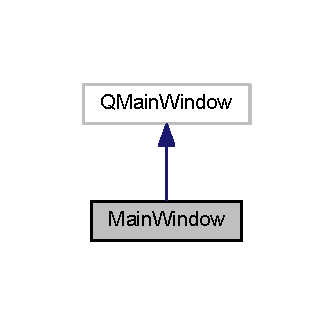
\includegraphics[width=160pt]{df/d61/a00031}
\end{center}
\end{figure}


Collaboration diagram for Main\+Window\+:\nopagebreak
\begin{figure}[H]
\begin{center}
\leavevmode
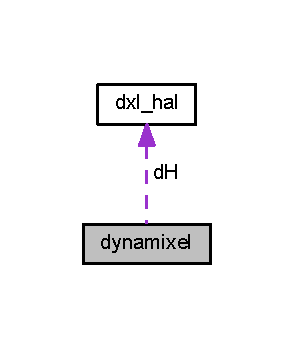
\includegraphics[width=248pt]{dc/d87/a00032}
\end{center}
\end{figure}
\subsection*{Signals}
\begin{DoxyCompactItemize}
\item 
void \hyperlink{a00005_ac85ba5aec3be2a51a348ff669b9dc842}{joystick\+Changed} ()
\begin{DoxyCompactList}\small\item\em Emmitted when a joystick changes. \end{DoxyCompactList}\end{DoxyCompactItemize}
\subsection*{Public Member Functions}
\begin{DoxyCompactItemize}
\item 
\hyperlink{a00005_a8b244be8b7b7db1b08de2a2acb9409db}{Main\+Window} (Q\+Widget $\ast$parent=0)
\begin{DoxyCompactList}\small\item\em Default constructor. \end{DoxyCompactList}\item 
\hyperlink{a00005_ae98d00a93bc118200eeef9f9bba1dba7}{$\sim$\+Main\+Window} ()
\begin{DoxyCompactList}\small\item\em Default destructor. \end{DoxyCompactList}\end{DoxyCompactItemize}
\subsection*{Private Types}
\begin{DoxyCompactItemize}
\item 
enum \hyperlink{a00005_a355d9f17965e5105226409313743cb9d}{Version} \{ \hyperlink{a00005_a355d9f17965e5105226409313743cb9daac0c8ddcec40274ec60fb95f59ba7aba}{v\+\_\+1\+\_\+0}
 \}
\end{DoxyCompactItemize}
\subsection*{Private Slots}
\begin{DoxyCompactItemize}
\item 
void \hyperlink{a00005_abb4c2d8a79c9f80010ea031366bf8226}{joy\+Changed} ()
\begin{DoxyCompactList}\small\item\em Handles a joystick update. \end{DoxyCompactList}\item 
void \hyperlink{a00005_a1dd57ccb62bc6f5a361aba6e088dd2e1}{on\+\_\+action\+Options\+\_\+triggered} ()
\begin{DoxyCompactList}\small\item\em To select the options. \end{DoxyCompactList}\item 
void \hyperlink{a00005_a128f71880d4b9683149023fc46fcc9f8}{update} ()
\begin{DoxyCompactList}\small\item\em Updates all data to the servo thread. \end{DoxyCompactList}\item 
void \hyperlink{a00005_ae66e9ab15f911b93fce0f161d2fde880}{on\+\_\+start\+\_\+clicked} ()
\end{DoxyCompactItemize}
\subsection*{Private Member Functions}
\begin{DoxyCompactItemize}
\item 
void \hyperlink{a00005_a6fd62e117414acda4fe6a93c453dfb93}{write} ()
\begin{DoxyCompactList}\small\item\em Writes the data to the default location. \end{DoxyCompactList}\item 
void \hyperlink{a00005_aa1362f75c2c485c0094c564256182641}{write} (Q\+String path)
\begin{DoxyCompactList}\small\item\em Writes the data to disk overloaded function. \end{DoxyCompactList}\end{DoxyCompactItemize}
\subsection*{Private Attributes}
\begin{DoxyCompactItemize}
\item 
Q\+Vector$<$ Q\+Label $\ast$ $>$ \hyperlink{a00005_a30c99d7a544f74b0650758e5cc7ead5a}{\+\_\+axis}
\begin{DoxyCompactList}\small\item\em Handles all the axis labels. \end{DoxyCompactList}\item 
Q\+Vector$<$ float $>$ \hyperlink{a00005_a20f66f574ed4c96d8dfc0013e1095f15}{\+\_\+axis\+V}
\begin{DoxyCompactList}\small\item\em Contains the axis value;. \end{DoxyCompactList}\item 
Q\+Vector$<$ Q\+Label $\ast$ $>$ \hyperlink{a00005_a8eaf474e1b8672f32873ed009e28ce8a}{\+\_\+buts}
\begin{DoxyCompactList}\small\item\em Handles all the button labels. \end{DoxyCompactList}\item 
Q\+Vector$<$ bool $>$ \hyperlink{a00005_a519ae4630572cb63fbd04bce12fe8e77}{\+\_\+buts\+V}
\begin{DoxyCompactList}\small\item\em Handles all buttons values. \end{DoxyCompactList}\item 
Q\+String \hyperlink{a00005_aaccbe653019df03668429890e325ac21}{\+\_\+data\+P}
\begin{DoxyCompactList}\small\item\em Contains the path to the data location. \end{DoxyCompactList}\item 
int \hyperlink{a00005_a282d4090e96c676578c4336391b1af08}{\+\_\+j\+Axis\+X} = -\/1
\begin{DoxyCompactList}\small\item\em Axis for the X value. \end{DoxyCompactList}\item 
int \hyperlink{a00005_aaaced09ce813bbcac92047f5ef39f182}{\+\_\+j\+Axis\+Y} = -\/1
\begin{DoxyCompactList}\small\item\em Axis for the Y value. \end{DoxyCompactList}\item 
int \hyperlink{a00005_a18cc17eff4ff04ee0aae07c609e82d33}{\+\_\+j\+Axis\+Z} = -\/1
\begin{DoxyCompactList}\small\item\em A\+Xis for the Z value. \end{DoxyCompactList}\item 
X\+Joystick \hyperlink{a00005_a671f35800890e518713e1946671d8730}{\+\_\+joy}
\begin{DoxyCompactList}\small\item\em To handle the joystick. \end{DoxyCompactList}\item 
\hyperlink{a00008}{Servo\+Thread} \hyperlink{a00005_a97f8ecc7ecb930b796178cef7b975013}{\+\_\+s\+T}
\begin{DoxyCompactList}\small\item\em Contains the thread controlling all the servos and external hardware. \end{DoxyCompactList}\item 
Q\+Timer \hyperlink{a00005_a254b03b878cfda75c1c411a2f8568d33}{\+\_\+timer}
\begin{DoxyCompactList}\small\item\em To update the joystick value. \end{DoxyCompactList}\item 
Ui\+::\+Main\+Window $\ast$ \hyperlink{a00005_a35466a70ed47252a0191168126a352a5}{ui}
\begin{DoxyCompactList}\small\item\em Contains the user interface. \end{DoxyCompactList}\end{DoxyCompactItemize}
\subsection*{Static Private Attributes}
\begin{DoxyCompactItemize}
\item 
static const int \hyperlink{a00005_a646727b1c45c72638325adfd460649c0}{s\+Count} = 3
\begin{DoxyCompactList}\small\item\em Contains the number of minimun servos to work. \end{DoxyCompactList}\item 
static const int \hyperlink{a00005_a42c44af9c0eebc33f4e81f02e15b0461}{a\+S\+Count} = 0
\begin{DoxyCompactList}\small\item\em Contains the number of additional servos used. \end{DoxyCompactList}\end{DoxyCompactItemize}


\subsection{Detailed Description}
Contains all the windows and other classes. 

\subsection{Member Enumeration Documentation}
\hypertarget{a00005_a355d9f17965e5105226409313743cb9d}{}\index{Main\+Window@{Main\+Window}!Version@{Version}}
\index{Version@{Version}!Main\+Window@{Main\+Window}}
\subsubsection[{Version}]{\setlength{\rightskip}{0pt plus 5cm}enum {\bf Main\+Window\+::\+Version}\hspace{0.3cm}{\ttfamily [private]}}\label{a00005_a355d9f17965e5105226409313743cb9d}
\begin{Desc}
\item[Enumerator]\par
\begin{description}
\index{v\+\_\+1\+\_\+0@{v\+\_\+1\+\_\+0}!Main\+Window@{Main\+Window}}\index{Main\+Window@{Main\+Window}!v\+\_\+1\+\_\+0@{v\+\_\+1\+\_\+0}}\item[{\em 
\hypertarget{a00005_a355d9f17965e5105226409313743cb9daac0c8ddcec40274ec60fb95f59ba7aba}{}v\+\_\+1\+\_\+0\label{a00005_a355d9f17965e5105226409313743cb9daac0c8ddcec40274ec60fb95f59ba7aba}
}]\end{description}
\end{Desc}

\begin{DoxyCode}
00032                  \{
00033         \hyperlink{a00005_a355d9f17965e5105226409313743cb9daac0c8ddcec40274ec60fb95f59ba7aba}{v\_1\_0}
00034     \};
\end{DoxyCode}


\subsection{Constructor \& Destructor Documentation}
\hypertarget{a00005_a8b244be8b7b7db1b08de2a2acb9409db}{}\index{Main\+Window@{Main\+Window}!Main\+Window@{Main\+Window}}
\index{Main\+Window@{Main\+Window}!Main\+Window@{Main\+Window}}
\subsubsection[{Main\+Window}]{\setlength{\rightskip}{0pt plus 5cm}Main\+Window\+::\+Main\+Window (
\begin{DoxyParamCaption}
\item[{Q\+Widget $\ast$}]{parent = {\ttfamily 0}}
\end{DoxyParamCaption}
)\hspace{0.3cm}{\ttfamily [explicit]}}\label{a00005_a8b244be8b7b7db1b08de2a2acb9409db}


Default constructor. 


\begin{DoxyCode}
00005                                       :
00006     QMainWindow(parent),
00007     \hyperlink{a00005_a30c99d7a544f74b0650758e5cc7ead5a}{\_axis}(XJoystick::AxisCount),
00008     \hyperlink{a00005_a20f66f574ed4c96d8dfc0013e1095f15}{\_axisV}(XJoystick::AxisCount),
00009     \hyperlink{a00005_a8eaf474e1b8672f32873ed009e28ce8a}{\_buts}(XJoystick::ButtonCount),
00010     \hyperlink{a00005_a519ae4630572cb63fbd04bce12fe8e77}{\_butsV}(XJoystick::ButtonCount),
00011     \hyperlink{a00005_a35466a70ed47252a0191168126a352a5}{ui}(\textcolor{keyword}{new} Ui::MainWindow)
00012 \{
00013     \hyperlink{a00005_a35466a70ed47252a0191168126a352a5}{ui}->setupUi(\textcolor{keyword}{this});
00014     
00015     \hyperlink{a00005_a97f8ecc7ecb930b796178cef7b975013}{\_sT}.start();
00016     
00017     connect(&\hyperlink{a00005_a671f35800890e518713e1946671d8730}{\_joy}, SIGNAL(changed()), \textcolor{keyword}{this}, SLOT(\hyperlink{a00005_abb4c2d8a79c9f80010ea031366bf8226}{joyChanged}()));
00018     connect(&\hyperlink{a00005_a254b03b878cfda75c1c411a2f8568d33}{\_timer}, SIGNAL(timeout()), \textcolor{keyword}{this}, SLOT(\hyperlink{a00005_a128f71880d4b9683149023fc46fcc9f8}{update}()));
00019     connect(&\hyperlink{a00005_a97f8ecc7ecb930b796178cef7b975013}{\_sT}, SIGNAL(statusBar(QString)), 
00020             \hyperlink{a00005_a35466a70ed47252a0191168126a352a5}{ui}->statusbar, SLOT(showMessage(QString)));
00021     
00022     
00023     \hyperlink{a00005_a254b03b878cfda75c1c411a2f8568d33}{\_timer}.setInterval(10);
00024     \hyperlink{a00005_a254b03b878cfda75c1c411a2f8568d33}{\_timer}.start();
00025     
00026     \textcolor{comment}{// JOYSTICK}
00027     QVector< QString > V(\hyperlink{a00005_a671f35800890e518713e1946671d8730}{\_joy}.getAllAxis());
00028     \textcolor{comment}{// Adding axis}
00029     QGridLayout *wL = \textcolor{keyword}{new} QGridLayout;
00030     \textcolor{keywordflow}{for} (\textcolor{keywordtype}{int} i = 0; i < XJoystick::AxisCount; ++i) \{
00031         QHBoxLayout *L = \textcolor{keyword}{new} QHBoxLayout;
00032         L->addWidget(\textcolor{keyword}{new} QLabel(V[i].append(\textcolor{stringliteral}{":"}), \textcolor{keyword}{this}));
00033         \hyperlink{a00005_a30c99d7a544f74b0650758e5cc7ead5a}{\_axis}[i] = \textcolor{keyword}{new} QLabel(\textcolor{stringliteral}{"#"});
00034         L->addWidget(\hyperlink{a00005_a30c99d7a544f74b0650758e5cc7ead5a}{\_axis}[i]);
00035         L->addStretch();
00036         wL->addLayout(L, i%3, i/3); 
00037     \}
00038     \hyperlink{a00005_a35466a70ed47252a0191168126a352a5}{ui}->joyAxis->setLayout(wL);
00039     
00040     \textcolor{comment}{// Adding buttons}
00041     wL = \textcolor{keyword}{new} QGridLayout;
00042     \textcolor{keywordflow}{for} (\textcolor{keywordtype}{int} i = 0; i < XJoystick::ButtonCount; ++i) \{
00043         \hyperlink{a00005_a8eaf474e1b8672f32873ed009e28ce8a}{\_buts}[i] = \textcolor{keyword}{new} QLabel(QString::number(i + 1));
00044         wL->addWidget(\hyperlink{a00005_a8eaf474e1b8672f32873ed009e28ce8a}{\_buts}[i], i/8, i%8);
00045         \hyperlink{a00005_a8eaf474e1b8672f32873ed009e28ce8a}{\_buts}[i]->setEnabled(\textcolor{keyword}{false});
00046         \hyperlink{a00005_a8eaf474e1b8672f32873ed009e28ce8a}{\_buts}[i]->hide();
00047     \}
00048     \hyperlink{a00005_a35466a70ed47252a0191168126a352a5}{ui}->joyButs->setLayout(wL);
00049     \hyperlink{a00005_a35466a70ed47252a0191168126a352a5}{ui}->joyAxis->hide();
00050     \hyperlink{a00005_a35466a70ed47252a0191168126a352a5}{ui}->joyButs->hide();
00051     \hyperlink{a00005_a35466a70ed47252a0191168126a352a5}{ui}->line->hide();
00052     
00053     
00054     \textcolor{comment}{// Creating data Path    }
00055     \hyperlink{a00005_aaccbe653019df03668429890e325ac21}{\_dataP} = QStandardPaths::writableLocation(QStandardPaths::AppDataLocation);
00056     QDir dir(\hyperlink{a00005_aaccbe653019df03668429890e325ac21}{\_dataP});
00057     \textcolor{keywordflow}{if} (!dir.exists()) dir.mkpath(\hyperlink{a00005_aaccbe653019df03668429890e325ac21}{\_dataP});
00058 \}
\end{DoxyCode}
\hypertarget{a00005_ae98d00a93bc118200eeef9f9bba1dba7}{}\index{Main\+Window@{Main\+Window}!````~Main\+Window@{$\sim$\+Main\+Window}}
\index{````~Main\+Window@{$\sim$\+Main\+Window}!Main\+Window@{Main\+Window}}
\subsubsection[{$\sim$\+Main\+Window}]{\setlength{\rightskip}{0pt plus 5cm}Main\+Window\+::$\sim$\+Main\+Window (
\begin{DoxyParamCaption}
{}
\end{DoxyParamCaption}
)}\label{a00005_ae98d00a93bc118200eeef9f9bba1dba7}


Default destructor. 


\begin{DoxyCode}
00061 \{
00062     \textcolor{keyword}{delete} \hyperlink{a00005_a35466a70ed47252a0191168126a352a5}{ui};
00063 \}
\end{DoxyCode}


\subsection{Member Function Documentation}
\hypertarget{a00005_abb4c2d8a79c9f80010ea031366bf8226}{}\index{Main\+Window@{Main\+Window}!joy\+Changed@{joy\+Changed}}
\index{joy\+Changed@{joy\+Changed}!Main\+Window@{Main\+Window}}
\subsubsection[{joy\+Changed}]{\setlength{\rightskip}{0pt plus 5cm}void Main\+Window\+::joy\+Changed (
\begin{DoxyParamCaption}
{}
\end{DoxyParamCaption}
)\hspace{0.3cm}{\ttfamily [private]}, {\ttfamily [slot]}}\label{a00005_abb4c2d8a79c9f80010ea031366bf8226}


Handles a joystick update. 


\begin{DoxyCode}
00081 \{
00082     \textcolor{keywordtype}{int} sel = \hyperlink{a00005_a671f35800890e518713e1946671d8730}{\_joy}.current();
00083     
00084     QVector< XJoystick::Info > V(\hyperlink{a00005_a671f35800890e518713e1946671d8730}{\_joy}.available());
00085     \textcolor{keywordtype}{bool} found = \textcolor{keyword}{false};
00086     \textcolor{keywordtype}{int} i = 0;
00087     \textcolor{keywordflow}{while} (i < V.size() and not found) \{ found = V[i].ID == sel; ++i; \}
00088     \textcolor{keywordflow}{if} (not found) \{
00089         \textcolor{keywordflow}{if} (V.size() > 0) \{
00090             \hyperlink{a00005_a671f35800890e518713e1946671d8730}{\_joy}.select(V[0].ID);
00091             \hyperlink{a00005_a35466a70ed47252a0191168126a352a5}{ui}->line->hide();
00092             
00093             \textcolor{comment}{// Showing axis}
00094             \hyperlink{a00005_a35466a70ed47252a0191168126a352a5}{ui}->joyAxis->show();
00095             
00096             \textcolor{comment}{// Showing buttons}
00097             \textcolor{keywordflow}{for} (QLabel *l : \hyperlink{a00005_a8eaf474e1b8672f32873ed009e28ce8a}{\_buts}) l->hide();
00098             \hyperlink{a00005_a35466a70ed47252a0191168126a352a5}{ui}->joyButs->show();
00099             \textcolor{keywordtype}{int} n = \hyperlink{a00005_a671f35800890e518713e1946671d8730}{\_joy}.buttonCount();
00100             \textcolor{keywordflow}{for} (\textcolor{keywordtype}{int} i = 0; i < n; ++i) \_buts[i]->show();
00101         \}
00102         \textcolor{keywordflow}{else} \{
00103             \hyperlink{a00005_a671f35800890e518713e1946671d8730}{\_joy}.select(-1);
00104             \hyperlink{a00005_a35466a70ed47252a0191168126a352a5}{ui}->joyAxis->hide();
00105             \hyperlink{a00005_a35466a70ed47252a0191168126a352a5}{ui}->joyButs->hide();
00106             \hyperlink{a00005_a35466a70ed47252a0191168126a352a5}{ui}->line->hide();
00107         \}
00108     \}
00109     emit \hyperlink{a00005_ac85ba5aec3be2a51a348ff669b9dc842}{joystickChanged}();
00110 \}
\end{DoxyCode}
\hypertarget{a00005_ac85ba5aec3be2a51a348ff669b9dc842}{}\index{Main\+Window@{Main\+Window}!joystick\+Changed@{joystick\+Changed}}
\index{joystick\+Changed@{joystick\+Changed}!Main\+Window@{Main\+Window}}
\subsubsection[{joystick\+Changed}]{\setlength{\rightskip}{0pt plus 5cm}void Main\+Window\+::joystick\+Changed (
\begin{DoxyParamCaption}
{}
\end{DoxyParamCaption}
)\hspace{0.3cm}{\ttfamily [signal]}}\label{a00005_ac85ba5aec3be2a51a348ff669b9dc842}


Emmitted when a joystick changes. 

\hypertarget{a00005_a1dd57ccb62bc6f5a361aba6e088dd2e1}{}\index{Main\+Window@{Main\+Window}!on\+\_\+action\+Options\+\_\+triggered@{on\+\_\+action\+Options\+\_\+triggered}}
\index{on\+\_\+action\+Options\+\_\+triggered@{on\+\_\+action\+Options\+\_\+triggered}!Main\+Window@{Main\+Window}}
\subsubsection[{on\+\_\+action\+Options\+\_\+triggered}]{\setlength{\rightskip}{0pt plus 5cm}void Main\+Window\+::on\+\_\+action\+Options\+\_\+triggered (
\begin{DoxyParamCaption}
{}
\end{DoxyParamCaption}
)\hspace{0.3cm}{\ttfamily [private]}, {\ttfamily [slot]}}\label{a00005_a1dd57ccb62bc6f5a361aba6e088dd2e1}


To select the options. 


\begin{DoxyCode}
00114 \{
00115     \hyperlink{a00006}{OptionsWindow} o(\hyperlink{a00005_a671f35800890e518713e1946671d8730}{\_joy}, &\hyperlink{a00005_a97f8ecc7ecb930b796178cef7b975013}{\_sT}, \hyperlink{a00005_a282d4090e96c676578c4336391b1af08}{\_jAxisX}, \hyperlink{a00005_aaaced09ce813bbcac92047f5ef39f182}{\_jAxisY}, 
      \hyperlink{a00005_a18cc17eff4ff04ee0aae07c609e82d33}{\_jAxisZ}, \textcolor{keyword}{this});
00116     o.exec();
00117     
00118     connect(\textcolor{keyword}{this}, SIGNAL(\hyperlink{a00005_ac85ba5aec3be2a51a348ff669b9dc842}{joystickChanged}()), &o, SLOT(
      \hyperlink{a00005_ac85ba5aec3be2a51a348ff669b9dc842}{joystickChanged}()));
00119     
00120     \textcolor{keywordflow}{if} (o.result()) o.storeData();
00121 \}
\end{DoxyCode}
\hypertarget{a00005_ae66e9ab15f911b93fce0f161d2fde880}{}\index{Main\+Window@{Main\+Window}!on\+\_\+start\+\_\+clicked@{on\+\_\+start\+\_\+clicked}}
\index{on\+\_\+start\+\_\+clicked@{on\+\_\+start\+\_\+clicked}!Main\+Window@{Main\+Window}}
\subsubsection[{on\+\_\+start\+\_\+clicked}]{\setlength{\rightskip}{0pt plus 5cm}void Main\+Window\+::on\+\_\+start\+\_\+clicked (
\begin{DoxyParamCaption}
{}
\end{DoxyParamCaption}
)\hspace{0.3cm}{\ttfamily [private]}, {\ttfamily [slot]}}\label{a00005_ae66e9ab15f911b93fce0f161d2fde880}

\begin{DoxyCode}
00159 \{
00160     QString text = \hyperlink{a00005_a35466a70ed47252a0191168126a352a5}{ui}->start->text();
00161     
00162     \textcolor{keywordflow}{if} (text == \textcolor{stringliteral}{"Start"}) \{
00163         \hyperlink{a00005_a97f8ecc7ecb930b796178cef7b975013}{\_sT}.\hyperlink{a00008_a5f32574f843d76deffec45995028389b}{wakeUp}();
00164         \hyperlink{a00005_a35466a70ed47252a0191168126a352a5}{ui}->start->setText(\textcolor{stringliteral}{"Stop"});
00165     \}
00166     \textcolor{keywordflow}{else} \textcolor{keywordflow}{if} (text == \textcolor{stringliteral}{"Stop"}) \{
00167         \hyperlink{a00005_a97f8ecc7ecb930b796178cef7b975013}{\_sT}.\hyperlink{a00008_ae0d4a59954aafbe8cd85f9326e4fcdd0}{pause}();
00168         \hyperlink{a00005_a35466a70ed47252a0191168126a352a5}{ui}->start->setText(\textcolor{stringliteral}{"Start"});
00169     \}
00170 \}
\end{DoxyCode}
\hypertarget{a00005_a128f71880d4b9683149023fc46fcc9f8}{}\index{Main\+Window@{Main\+Window}!update@{update}}
\index{update@{update}!Main\+Window@{Main\+Window}}
\subsubsection[{update}]{\setlength{\rightskip}{0pt plus 5cm}void Main\+Window\+::update (
\begin{DoxyParamCaption}
{}
\end{DoxyParamCaption}
)\hspace{0.3cm}{\ttfamily [private]}, {\ttfamily [slot]}}\label{a00005_a128f71880d4b9683149023fc46fcc9f8}


Updates all data to the servo thread. 


\begin{DoxyCode}
00124 \{
00125     \textcolor{comment}{// Joystick values}
00126     \hyperlink{a00005_a671f35800890e518713e1946671d8730}{\_joy}.update();
00127     \textcolor{keywordflow}{for} (\textcolor{keywordtype}{int} i = 0; i < XJoystick::AxisCount; ++i) \{
00128         \textcolor{keywordtype}{float} temp = \hyperlink{a00005_a671f35800890e518713e1946671d8730}{\_joy}[i];
00129         \hyperlink{a00005_a20f66f574ed4c96d8dfc0013e1095f15}{\_axisV}[i] = temp;
00130         \hyperlink{a00005_a30c99d7a544f74b0650758e5cc7ead5a}{\_axis}[i]->setText(QString::number(temp));
00131     \}
00132     \textcolor{keywordflow}{for} (\textcolor{keywordtype}{int} i = 0; i < XJoystick::ButtonCount; ++i) \{
00133         \textcolor{keywordtype}{bool} temp = \hyperlink{a00005_a671f35800890e518713e1946671d8730}{\_joy}.button(i);
00134         \hyperlink{a00005_a519ae4630572cb63fbd04bce12fe8e77}{\_butsV}[i] = temp;
00135         \hyperlink{a00005_a8eaf474e1b8672f32873ed009e28ce8a}{\_buts}[i]->setEnabled(temp);
00136     \}
00137     
00138     \hyperlink{a00005_a97f8ecc7ecb930b796178cef7b975013}{\_sT}.\hyperlink{a00008_a8497ea56991b620981ce1fbf53d9ebdb}{setData}(\hyperlink{a00005_a20f66f574ed4c96d8dfc0013e1095f15}{\_axisV}, \hyperlink{a00005_a519ae4630572cb63fbd04bce12fe8e77}{\_butsV});
00139     QVector<ServoThread::Servo> servo(\hyperlink{a00005_a97f8ecc7ecb930b796178cef7b975013}{\_sT}.\hyperlink{a00008_a5fd8ef13314428f5ba7646730cc58f1c}{getServosInfo}());
00140     
00141     \textcolor{comment}{// Updating position sliders}
00142     \hyperlink{a00005_a35466a70ed47252a0191168126a352a5}{ui}->servo0S->setValue(servo[0].pos);
00143     \hyperlink{a00005_a35466a70ed47252a0191168126a352a5}{ui}->servo1S->setValue(servo[1].pos);
00144     \hyperlink{a00005_a35466a70ed47252a0191168126a352a5}{ui}->servo2S->setValue(servo[2].pos);
00145     
00146     \textcolor{comment}{// Updating position labels}
00147     \hyperlink{a00005_a35466a70ed47252a0191168126a352a5}{ui}->servo0->setText(QString::number(servo[0].pos));
00148     \hyperlink{a00005_a35466a70ed47252a0191168126a352a5}{ui}->servo1->setText(QString::number(servo[1].pos));
00149     \hyperlink{a00005_a35466a70ed47252a0191168126a352a5}{ui}->servo2->setText(QString::number(servo[2].pos));
00150     
00151     \textcolor{comment}{// Updating load labels}
00152     \hyperlink{a00005_a35466a70ed47252a0191168126a352a5}{ui}->servo0L->setText(QString::number(servo[0].load));
00153     \hyperlink{a00005_a35466a70ed47252a0191168126a352a5}{ui}->servo1L->setText(QString::number(servo[1].load));
00154     \hyperlink{a00005_a35466a70ed47252a0191168126a352a5}{ui}->servo2L->setText(QString::number(servo[2].load));
00155     
00156 \}
\end{DoxyCode}
\hypertarget{a00005_a6fd62e117414acda4fe6a93c453dfb93}{}\index{Main\+Window@{Main\+Window}!write@{write}}
\index{write@{write}!Main\+Window@{Main\+Window}}
\subsubsection[{write}]{\setlength{\rightskip}{0pt plus 5cm}void Main\+Window\+::write (
\begin{DoxyParamCaption}
{}
\end{DoxyParamCaption}
)\hspace{0.3cm}{\ttfamily [inline]}, {\ttfamily [private]}}\label{a00005_a6fd62e117414acda4fe6a93c453dfb93}


Writes the data to the default location. 


\begin{DoxyCode}
00083 \{ \hyperlink{a00005_a6fd62e117414acda4fe6a93c453dfb93}{write}(\hyperlink{a00005_aaccbe653019df03668429890e325ac21}{\_dataP}); \}
\end{DoxyCode}
\hypertarget{a00005_aa1362f75c2c485c0094c564256182641}{}\index{Main\+Window@{Main\+Window}!write@{write}}
\index{write@{write}!Main\+Window@{Main\+Window}}
\subsubsection[{write}]{\setlength{\rightskip}{0pt plus 5cm}void Main\+Window\+::write (
\begin{DoxyParamCaption}
\item[{Q\+String}]{path}
\end{DoxyParamCaption}
)\hspace{0.3cm}{\ttfamily [private]}}\label{a00005_aa1362f75c2c485c0094c564256182641}


Writes the data to disk overloaded function. 


\begin{DoxyCode}
00066 \{
00067     QDir dir(path);
00068     QFile file(dir.filePath(\textcolor{stringliteral}{"main.opts"}));
00069     \textcolor{keywordflow}{if}(not file.open(QIODevice::WriteOnly)) \{
00070         \hyperlink{a00005_a35466a70ed47252a0191168126a352a5}{ui}->statusbar->showMessage(\textcolor{stringliteral}{"Error saving file"}, 1000);
00071         \textcolor{keywordflow}{return};
00072     \}
00073     
00074     QDataStream f(&file);
00075     f << int(Version::v\_1\_0) << \hyperlink{a00005_a282d4090e96c676578c4336391b1af08}{\_jAxisX} << \hyperlink{a00005_aaaced09ce813bbcac92047f5ef39f182}{\_jAxisY} << \hyperlink{a00005_a18cc17eff4ff04ee0aae07c609e82d33}{\_jAxisZ};
00076     
00077     \hyperlink{a00005_a97f8ecc7ecb930b796178cef7b975013}{\_sT}.\hyperlink{a00008_aca68fe85a100a052c4d41f0fa88cc152}{write}(dir.filePath(\textcolor{stringliteral}{"servo.opts"}));
00078 \}
\end{DoxyCode}


\subsection{Member Data Documentation}
\hypertarget{a00005_a30c99d7a544f74b0650758e5cc7ead5a}{}\index{Main\+Window@{Main\+Window}!\+\_\+axis@{\+\_\+axis}}
\index{\+\_\+axis@{\+\_\+axis}!Main\+Window@{Main\+Window}}
\subsubsection[{\+\_\+axis}]{\setlength{\rightskip}{0pt plus 5cm}Q\+Vector$<$ Q\+Label $\ast$$>$ Main\+Window\+::\+\_\+axis\hspace{0.3cm}{\ttfamily [private]}}\label{a00005_a30c99d7a544f74b0650758e5cc7ead5a}


Handles all the axis labels. 

\hypertarget{a00005_a20f66f574ed4c96d8dfc0013e1095f15}{}\index{Main\+Window@{Main\+Window}!\+\_\+axis\+V@{\+\_\+axis\+V}}
\index{\+\_\+axis\+V@{\+\_\+axis\+V}!Main\+Window@{Main\+Window}}
\subsubsection[{\+\_\+axis\+V}]{\setlength{\rightskip}{0pt plus 5cm}Q\+Vector$<$ float $>$ Main\+Window\+::\+\_\+axis\+V\hspace{0.3cm}{\ttfamily [private]}}\label{a00005_a20f66f574ed4c96d8dfc0013e1095f15}


Contains the axis value;. 

\hypertarget{a00005_a8eaf474e1b8672f32873ed009e28ce8a}{}\index{Main\+Window@{Main\+Window}!\+\_\+buts@{\+\_\+buts}}
\index{\+\_\+buts@{\+\_\+buts}!Main\+Window@{Main\+Window}}
\subsubsection[{\+\_\+buts}]{\setlength{\rightskip}{0pt plus 5cm}Q\+Vector$<$ Q\+Label $\ast$$>$ Main\+Window\+::\+\_\+buts\hspace{0.3cm}{\ttfamily [private]}}\label{a00005_a8eaf474e1b8672f32873ed009e28ce8a}


Handles all the button labels. 

\hypertarget{a00005_a519ae4630572cb63fbd04bce12fe8e77}{}\index{Main\+Window@{Main\+Window}!\+\_\+buts\+V@{\+\_\+buts\+V}}
\index{\+\_\+buts\+V@{\+\_\+buts\+V}!Main\+Window@{Main\+Window}}
\subsubsection[{\+\_\+buts\+V}]{\setlength{\rightskip}{0pt plus 5cm}Q\+Vector$<$ bool $>$ Main\+Window\+::\+\_\+buts\+V\hspace{0.3cm}{\ttfamily [private]}}\label{a00005_a519ae4630572cb63fbd04bce12fe8e77}


Handles all buttons values. 

\hypertarget{a00005_aaccbe653019df03668429890e325ac21}{}\index{Main\+Window@{Main\+Window}!\+\_\+data\+P@{\+\_\+data\+P}}
\index{\+\_\+data\+P@{\+\_\+data\+P}!Main\+Window@{Main\+Window}}
\subsubsection[{\+\_\+data\+P}]{\setlength{\rightskip}{0pt plus 5cm}Q\+String Main\+Window\+::\+\_\+data\+P\hspace{0.3cm}{\ttfamily [private]}}\label{a00005_aaccbe653019df03668429890e325ac21}


Contains the path to the data location. 

\hypertarget{a00005_a282d4090e96c676578c4336391b1af08}{}\index{Main\+Window@{Main\+Window}!\+\_\+j\+Axis\+X@{\+\_\+j\+Axis\+X}}
\index{\+\_\+j\+Axis\+X@{\+\_\+j\+Axis\+X}!Main\+Window@{Main\+Window}}
\subsubsection[{\+\_\+j\+Axis\+X}]{\setlength{\rightskip}{0pt plus 5cm}int Main\+Window\+::\+\_\+j\+Axis\+X = -\/1\hspace{0.3cm}{\ttfamily [private]}}\label{a00005_a282d4090e96c676578c4336391b1af08}


Axis for the X value. 

\hypertarget{a00005_aaaced09ce813bbcac92047f5ef39f182}{}\index{Main\+Window@{Main\+Window}!\+\_\+j\+Axis\+Y@{\+\_\+j\+Axis\+Y}}
\index{\+\_\+j\+Axis\+Y@{\+\_\+j\+Axis\+Y}!Main\+Window@{Main\+Window}}
\subsubsection[{\+\_\+j\+Axis\+Y}]{\setlength{\rightskip}{0pt plus 5cm}int Main\+Window\+::\+\_\+j\+Axis\+Y = -\/1\hspace{0.3cm}{\ttfamily [private]}}\label{a00005_aaaced09ce813bbcac92047f5ef39f182}


Axis for the Y value. 

\hypertarget{a00005_a18cc17eff4ff04ee0aae07c609e82d33}{}\index{Main\+Window@{Main\+Window}!\+\_\+j\+Axis\+Z@{\+\_\+j\+Axis\+Z}}
\index{\+\_\+j\+Axis\+Z@{\+\_\+j\+Axis\+Z}!Main\+Window@{Main\+Window}}
\subsubsection[{\+\_\+j\+Axis\+Z}]{\setlength{\rightskip}{0pt plus 5cm}int Main\+Window\+::\+\_\+j\+Axis\+Z = -\/1\hspace{0.3cm}{\ttfamily [private]}}\label{a00005_a18cc17eff4ff04ee0aae07c609e82d33}


A\+Xis for the Z value. 

\hypertarget{a00005_a671f35800890e518713e1946671d8730}{}\index{Main\+Window@{Main\+Window}!\+\_\+joy@{\+\_\+joy}}
\index{\+\_\+joy@{\+\_\+joy}!Main\+Window@{Main\+Window}}
\subsubsection[{\+\_\+joy}]{\setlength{\rightskip}{0pt plus 5cm}X\+Joystick Main\+Window\+::\+\_\+joy\hspace{0.3cm}{\ttfamily [private]}}\label{a00005_a671f35800890e518713e1946671d8730}


To handle the joystick. 

\hypertarget{a00005_a97f8ecc7ecb930b796178cef7b975013}{}\index{Main\+Window@{Main\+Window}!\+\_\+s\+T@{\+\_\+s\+T}}
\index{\+\_\+s\+T@{\+\_\+s\+T}!Main\+Window@{Main\+Window}}
\subsubsection[{\+\_\+s\+T}]{\setlength{\rightskip}{0pt plus 5cm}{\bf Servo\+Thread} Main\+Window\+::\+\_\+s\+T\hspace{0.3cm}{\ttfamily [private]}}\label{a00005_a97f8ecc7ecb930b796178cef7b975013}


Contains the thread controlling all the servos and external hardware. 

\hypertarget{a00005_a254b03b878cfda75c1c411a2f8568d33}{}\index{Main\+Window@{Main\+Window}!\+\_\+timer@{\+\_\+timer}}
\index{\+\_\+timer@{\+\_\+timer}!Main\+Window@{Main\+Window}}
\subsubsection[{\+\_\+timer}]{\setlength{\rightskip}{0pt plus 5cm}Q\+Timer Main\+Window\+::\+\_\+timer\hspace{0.3cm}{\ttfamily [private]}}\label{a00005_a254b03b878cfda75c1c411a2f8568d33}


To update the joystick value. 

\hypertarget{a00005_a42c44af9c0eebc33f4e81f02e15b0461}{}\index{Main\+Window@{Main\+Window}!a\+S\+Count@{a\+S\+Count}}
\index{a\+S\+Count@{a\+S\+Count}!Main\+Window@{Main\+Window}}
\subsubsection[{a\+S\+Count}]{\setlength{\rightskip}{0pt plus 5cm}const int Main\+Window\+::a\+S\+Count = 0\hspace{0.3cm}{\ttfamily [static]}, {\ttfamily [private]}}\label{a00005_a42c44af9c0eebc33f4e81f02e15b0461}


Contains the number of additional servos used. 

\hypertarget{a00005_a646727b1c45c72638325adfd460649c0}{}\index{Main\+Window@{Main\+Window}!s\+Count@{s\+Count}}
\index{s\+Count@{s\+Count}!Main\+Window@{Main\+Window}}
\subsubsection[{s\+Count}]{\setlength{\rightskip}{0pt plus 5cm}const int Main\+Window\+::s\+Count = 3\hspace{0.3cm}{\ttfamily [static]}, {\ttfamily [private]}}\label{a00005_a646727b1c45c72638325adfd460649c0}


Contains the number of minimun servos to work. 

\hypertarget{a00005_a35466a70ed47252a0191168126a352a5}{}\index{Main\+Window@{Main\+Window}!ui@{ui}}
\index{ui@{ui}!Main\+Window@{Main\+Window}}
\subsubsection[{ui}]{\setlength{\rightskip}{0pt plus 5cm}Ui\+::\+Main\+Window$\ast$ Main\+Window\+::ui\hspace{0.3cm}{\ttfamily [private]}}\label{a00005_a35466a70ed47252a0191168126a352a5}


Contains the user interface. 



The documentation for this class was generated from the following files\+:\begin{DoxyCompactItemize}
\item 
\hyperlink{a00017}{mainwindow.\+h}\item 
\hyperlink{a00016}{mainwindow.\+cpp}\end{DoxyCompactItemize}

\hypertarget{a00006}{}\section{Servo\+Thread\+:\+:Servo Struct Reference}
\label{a00006}\index{Servo\+Thread\+::\+Servo@{Servo\+Thread\+::\+Servo}}


Struct for the \hyperlink{a00001}{A\+X12} servos.  




{\ttfamily \#include $<$servothread.\+h$>$}

\subsection*{Public Member Functions}
\begin{DoxyCompactItemize}
\item 
\hyperlink{a00006_a031c8e78df1e5eddf80bd2b2e2998658}{Servo} (int \hyperlink{a00006_a06b514c42113aa85fd1703fc88fca7ce}{I\+D}=-\/1, double \hyperlink{a00006_ae378d77acf16b306649c87fdb8df677e}{load}=-\/1, double \hyperlink{a00006_a9fa0aa56944b9b0bb9d66303d5bd4b59}{pos}=-\/1)
\begin{DoxyCompactList}\small\item\em Default constructor. \end{DoxyCompactList}\item 
\hyperlink{a00006_acb657f09a5d04424d134791ca501cb54}{Servo} (const \hyperlink{a00006}{Servo} \&s)
\begin{DoxyCompactList}\small\item\em Copy constructor. \end{DoxyCompactList}\end{DoxyCompactItemize}
\subsection*{Public Attributes}
\begin{DoxyCompactItemize}
\item 
int \hyperlink{a00006_a06b514c42113aa85fd1703fc88fca7ce}{I\+D}
\begin{DoxyCompactList}\small\item\em Contains the servo I\+D. \end{DoxyCompactList}\item 
double \hyperlink{a00006_ae378d77acf16b306649c87fdb8df677e}{load}
\begin{DoxyCompactList}\small\item\em Contains the servo load. \end{DoxyCompactList}\item 
double \hyperlink{a00006_a9fa0aa56944b9b0bb9d66303d5bd4b59}{pos}
\begin{DoxyCompactList}\small\item\em Contains the servo position. \end{DoxyCompactList}\end{DoxyCompactItemize}


\subsection{Detailed Description}
Struct for the \hyperlink{a00001}{A\+X12} servos. 

\subsection{Constructor \& Destructor Documentation}
\hypertarget{a00006_a031c8e78df1e5eddf80bd2b2e2998658}{}\index{Servo\+Thread\+::\+Servo@{Servo\+Thread\+::\+Servo}!Servo@{Servo}}
\index{Servo@{Servo}!Servo\+Thread\+::\+Servo@{Servo\+Thread\+::\+Servo}}
\subsubsection[{Servo}]{\setlength{\rightskip}{0pt plus 5cm}Servo\+Thread\+::\+Servo\+::\+Servo (
\begin{DoxyParamCaption}
\item[{int}]{I\+D = {\ttfamily -\/1}, }
\item[{double}]{load = {\ttfamily -\/1}, }
\item[{double}]{pos = {\ttfamily -\/1}}
\end{DoxyParamCaption}
)\hspace{0.3cm}{\ttfamily [inline]}}\label{a00006_a031c8e78df1e5eddf80bd2b2e2998658}


Default constructor. 


\begin{DoxyCode}
00034             : \hyperlink{a00006_a06b514c42113aa85fd1703fc88fca7ce}{ID}(\hyperlink{a00006_a06b514c42113aa85fd1703fc88fca7ce}{ID}), \hyperlink{a00006_ae378d77acf16b306649c87fdb8df677e}{load}(\hyperlink{a00006_ae378d77acf16b306649c87fdb8df677e}{load}), \hyperlink{a00006_a9fa0aa56944b9b0bb9d66303d5bd4b59}{pos}(\hyperlink{a00006_a9fa0aa56944b9b0bb9d66303d5bd4b59}{pos}) \{\}
\end{DoxyCode}
\hypertarget{a00006_acb657f09a5d04424d134791ca501cb54}{}\index{Servo\+Thread\+::\+Servo@{Servo\+Thread\+::\+Servo}!Servo@{Servo}}
\index{Servo@{Servo}!Servo\+Thread\+::\+Servo@{Servo\+Thread\+::\+Servo}}
\subsubsection[{Servo}]{\setlength{\rightskip}{0pt plus 5cm}Servo\+Thread\+::\+Servo\+::\+Servo (
\begin{DoxyParamCaption}
\item[{const {\bf Servo} \&}]{s}
\end{DoxyParamCaption}
)\hspace{0.3cm}{\ttfamily [inline]}}\label{a00006_acb657f09a5d04424d134791ca501cb54}


Copy constructor. 


\begin{DoxyCode}
00037 : \hyperlink{a00006_a06b514c42113aa85fd1703fc88fca7ce}{ID}(s.ID), \hyperlink{a00006_ae378d77acf16b306649c87fdb8df677e}{load}(s.load), \hyperlink{a00006_a9fa0aa56944b9b0bb9d66303d5bd4b59}{pos}(s.pos) \{\}
\end{DoxyCode}


\subsection{Member Data Documentation}
\hypertarget{a00006_a06b514c42113aa85fd1703fc88fca7ce}{}\index{Servo\+Thread\+::\+Servo@{Servo\+Thread\+::\+Servo}!I\+D@{I\+D}}
\index{I\+D@{I\+D}!Servo\+Thread\+::\+Servo@{Servo\+Thread\+::\+Servo}}
\subsubsection[{I\+D}]{\setlength{\rightskip}{0pt plus 5cm}int Servo\+Thread\+::\+Servo\+::\+I\+D}\label{a00006_a06b514c42113aa85fd1703fc88fca7ce}


Contains the servo I\+D. 

\hypertarget{a00006_ae378d77acf16b306649c87fdb8df677e}{}\index{Servo\+Thread\+::\+Servo@{Servo\+Thread\+::\+Servo}!load@{load}}
\index{load@{load}!Servo\+Thread\+::\+Servo@{Servo\+Thread\+::\+Servo}}
\subsubsection[{load}]{\setlength{\rightskip}{0pt plus 5cm}double Servo\+Thread\+::\+Servo\+::load}\label{a00006_ae378d77acf16b306649c87fdb8df677e}


Contains the servo load. 

\hypertarget{a00006_a9fa0aa56944b9b0bb9d66303d5bd4b59}{}\index{Servo\+Thread\+::\+Servo@{Servo\+Thread\+::\+Servo}!pos@{pos}}
\index{pos@{pos}!Servo\+Thread\+::\+Servo@{Servo\+Thread\+::\+Servo}}
\subsubsection[{pos}]{\setlength{\rightskip}{0pt plus 5cm}double Servo\+Thread\+::\+Servo\+::pos}\label{a00006_a9fa0aa56944b9b0bb9d66303d5bd4b59}


Contains the servo position. 



The documentation for this struct was generated from the following file\+:\begin{DoxyCompactItemize}
\item 
\hyperlink{a00020}{servothread.\+h}\end{DoxyCompactItemize}

\hypertarget{a00007}{}\subsection{Servo\+Thread\+:\+:Servo Struct Reference}
\label{a00007}\index{Servo\+Thread\+::\+Servo@{Servo\+Thread\+::\+Servo}}


Struct for the \hyperlink{a00001}{A\+X12} servos.  




{\ttfamily \#include $<$servothread.\+h$>$}

\subsubsection*{Public Member Functions}
\begin{DoxyCompactItemize}
\item 
\hyperlink{a00007_a219887703cad3d3252fdde5a1aae586e}{Servo} (int \hyperlink{a00007_a06b514c42113aa85fd1703fc88fca7ce}{I\+D}=-\/1, double \hyperlink{a00007_a9fa0aa56944b9b0bb9d66303d5bd4b59}{pos}=-\/1)
\begin{DoxyCompactList}\small\item\em Default constructor. \end{DoxyCompactList}\item 
\hyperlink{a00007_acb657f09a5d04424d134791ca501cb54}{Servo} (const \hyperlink{a00007}{Servo} \&s)
\begin{DoxyCompactList}\small\item\em Copy constructor. \end{DoxyCompactList}\item 
void \hyperlink{a00007_acfe010f463ec6e85718a9883689811cb}{operator=} (const \hyperlink{a00007}{Servo} \&s)
\begin{DoxyCompactList}\small\item\em Operator overloading. \end{DoxyCompactList}\end{DoxyCompactItemize}
\subsubsection*{Public Attributes}
\begin{DoxyCompactItemize}
\item 
int \hyperlink{a00007_a06b514c42113aa85fd1703fc88fca7ce}{I\+D}
\begin{DoxyCompactList}\small\item\em Contains the servo I\+D. \end{DoxyCompactList}\item 
double \hyperlink{a00007_a9fa0aa56944b9b0bb9d66303d5bd4b59}{pos}
\begin{DoxyCompactList}\small\item\em Contains the servo position. \end{DoxyCompactList}\end{DoxyCompactItemize}


\subsubsection{Detailed Description}
Struct for the \hyperlink{a00001}{A\+X12} servos. 

\subsubsection{Constructor \& Destructor Documentation}
\hypertarget{a00007_a219887703cad3d3252fdde5a1aae586e}{}\index{Servo\+Thread\+::\+Servo@{Servo\+Thread\+::\+Servo}!Servo@{Servo}}
\index{Servo@{Servo}!Servo\+Thread\+::\+Servo@{Servo\+Thread\+::\+Servo}}
\paragraph[{Servo}]{\setlength{\rightskip}{0pt plus 5cm}Servo\+Thread\+::\+Servo\+::\+Servo (
\begin{DoxyParamCaption}
\item[{int}]{I\+D = {\ttfamily -\/1}, }
\item[{double}]{pos = {\ttfamily -\/1}}
\end{DoxyParamCaption}
)\hspace{0.3cm}{\ttfamily [inline]}}\label{a00007_a219887703cad3d3252fdde5a1aae586e}


Default constructor. 


\begin{DoxyCode}
00080             : \hyperlink{a00007_a06b514c42113aa85fd1703fc88fca7ce}{ID}(\hyperlink{a00007_a06b514c42113aa85fd1703fc88fca7ce}{ID}), \hyperlink{a00007_a9fa0aa56944b9b0bb9d66303d5bd4b59}{pos}(\hyperlink{a00007_a9fa0aa56944b9b0bb9d66303d5bd4b59}{pos}) \{\}
\end{DoxyCode}
\hypertarget{a00007_acb657f09a5d04424d134791ca501cb54}{}\index{Servo\+Thread\+::\+Servo@{Servo\+Thread\+::\+Servo}!Servo@{Servo}}
\index{Servo@{Servo}!Servo\+Thread\+::\+Servo@{Servo\+Thread\+::\+Servo}}
\paragraph[{Servo}]{\setlength{\rightskip}{0pt plus 5cm}Servo\+Thread\+::\+Servo\+::\+Servo (
\begin{DoxyParamCaption}
\item[{const {\bf Servo} \&}]{s}
\end{DoxyParamCaption}
)\hspace{0.3cm}{\ttfamily [inline]}}\label{a00007_acb657f09a5d04424d134791ca501cb54}


Copy constructor. 


\begin{DoxyCode}
00083 : \hyperlink{a00007_a06b514c42113aa85fd1703fc88fca7ce}{ID}(s.ID), \hyperlink{a00007_a9fa0aa56944b9b0bb9d66303d5bd4b59}{pos}(s.pos) \{\}
\end{DoxyCode}


\subsubsection{Member Function Documentation}
\hypertarget{a00007_acfe010f463ec6e85718a9883689811cb}{}\index{Servo\+Thread\+::\+Servo@{Servo\+Thread\+::\+Servo}!operator=@{operator=}}
\index{operator=@{operator=}!Servo\+Thread\+::\+Servo@{Servo\+Thread\+::\+Servo}}
\paragraph[{operator=}]{\setlength{\rightskip}{0pt plus 5cm}void Servo\+Thread\+::\+Servo\+::operator= (
\begin{DoxyParamCaption}
\item[{const {\bf Servo} \&}]{s}
\end{DoxyParamCaption}
)\hspace{0.3cm}{\ttfamily [inline]}}\label{a00007_acfe010f463ec6e85718a9883689811cb}


Operator overloading. 


\begin{DoxyCode}
00087         \{
00088             this->\hyperlink{a00007_a06b514c42113aa85fd1703fc88fca7ce}{ID} = s.ID;
00089             this->\hyperlink{a00007_a9fa0aa56944b9b0bb9d66303d5bd4b59}{pos} = s.pos;
00090         \}
\end{DoxyCode}


\subsubsection{Member Data Documentation}
\hypertarget{a00007_a06b514c42113aa85fd1703fc88fca7ce}{}\index{Servo\+Thread\+::\+Servo@{Servo\+Thread\+::\+Servo}!I\+D@{I\+D}}
\index{I\+D@{I\+D}!Servo\+Thread\+::\+Servo@{Servo\+Thread\+::\+Servo}}
\paragraph[{I\+D}]{\setlength{\rightskip}{0pt plus 5cm}int Servo\+Thread\+::\+Servo\+::\+I\+D}\label{a00007_a06b514c42113aa85fd1703fc88fca7ce}


Contains the servo I\+D. 

\hypertarget{a00007_a9fa0aa56944b9b0bb9d66303d5bd4b59}{}\index{Servo\+Thread\+::\+Servo@{Servo\+Thread\+::\+Servo}!pos@{pos}}
\index{pos@{pos}!Servo\+Thread\+::\+Servo@{Servo\+Thread\+::\+Servo}}
\paragraph[{pos}]{\setlength{\rightskip}{0pt plus 5cm}double Servo\+Thread\+::\+Servo\+::pos}\label{a00007_a9fa0aa56944b9b0bb9d66303d5bd4b59}


Contains the servo position. 



The documentation for this struct was generated from the following file\+:\begin{DoxyCompactItemize}
\item 
\hyperlink{a00024}{servothread.\+h}\end{DoxyCompactItemize}

\hypertarget{a00008}{}\section{Servo\+Find Class Reference}
\label{a00008}\index{Servo\+Find@{Servo\+Find}}


{\ttfamily \#include $<$servofind.\+h$>$}



Inheritance diagram for Servo\+Find\+:
\nopagebreak
\begin{figure}[H]
\begin{center}
\leavevmode
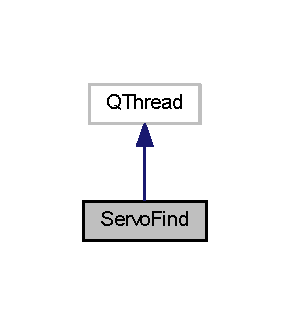
\includegraphics[width=139pt]{db/d3a/a00040}
\end{center}
\end{figure}


Collaboration diagram for Servo\+Find\+:
\nopagebreak
\begin{figure}[H]
\begin{center}
\leavevmode
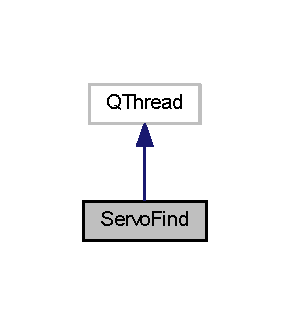
\includegraphics[width=139pt]{dd/d32/a00041}
\end{center}
\end{figure}
\subsection*{Signals}
\begin{DoxyCompactItemize}
\item 
void \hyperlink{a00008_a8ae9f951508e8376c3c7421df37ea619}{completion} (int)
\begin{DoxyCompactList}\small\item\em Shows the completion of the process. \end{DoxyCompactList}\end{DoxyCompactItemize}
\subsection*{Public Member Functions}
\begin{DoxyCompactItemize}
\item 
\hyperlink{a00008_ad9b1d82aecc71025fb606b79b9bf6ce1}{Servo\+Find} ()
\begin{DoxyCompactList}\small\item\em Default constructor. \end{DoxyCompactList}\item 
\hyperlink{a00008_a5f353598d5d40289c039412288e5bf73}{$\sim$\+Servo\+Find} ()
\begin{DoxyCompactList}\small\item\em Default destructor. \end{DoxyCompactList}\item 
void \hyperlink{a00008_a4edb0ac2852a93f84c6aa04d5953e28d}{run} ()
\begin{DoxyCompactList}\small\item\em Main function. \end{DoxyCompactList}\item 
void \hyperlink{a00008_a440f961980162cfd7c2ca9031b2a76e8}{set\+Data} (Q\+Vector$<$ Q\+Combo\+Box $\ast$ $>$ servo, Q\+String port, int baud, int min=0, int max=M\+A\+X\+\_\+\+I\+D)
\begin{DoxyCompactList}\small\item\em To set all data. \end{DoxyCompactList}\end{DoxyCompactItemize}
\subsection*{Private Types}
\begin{DoxyCompactItemize}
\item 
typedef Q\+Combo\+Box \hyperlink{a00008_a8cfdbef4d4dc51f1b200a885ff827711}{Q\+C\+B}
\end{DoxyCompactItemize}
\subsection*{Private Attributes}
\begin{DoxyCompactItemize}
\item 
int \hyperlink{a00008_ad2f3b1ab924ff2051178eb981d030b66}{\+\_\+baud}
\begin{DoxyCompactList}\small\item\em Contains the baud rate. \end{DoxyCompactList}\item 
int \hyperlink{a00008_a65a3d5606c9a8bcd6ace9be36c3551e1}{\+\_\+min} = 0
\begin{DoxyCompactList}\small\item\em Minimum value to find. \end{DoxyCompactList}\item 
int \hyperlink{a00008_abb4bcc300ab0a9c1df3c41b4e7d1fe2d}{\+\_\+max} = M\+A\+X\+\_\+\+I\+D
\begin{DoxyCompactList}\small\item\em Maximum value to find. \end{DoxyCompactList}\item 
Q\+String \hyperlink{a00008_acc6d9f94a8cf7a7a777fd9c818d98207}{\+\_\+port}
\begin{DoxyCompactList}\small\item\em Contains the current port. \end{DoxyCompactList}\item 
Q\+Vector$<$ Q\+Combo\+Box $\ast$ $>$ \hyperlink{a00008_a571ee1fc45255666e5baa0d5e9111551}{\+\_\+servo}
\begin{DoxyCompactList}\small\item\em Contains the pointer to the servos Q\+Combo\+Boxes. \end{DoxyCompactList}\end{DoxyCompactItemize}


\subsection{Member Typedef Documentation}
\hypertarget{a00008_a8cfdbef4d4dc51f1b200a885ff827711}{}\index{Servo\+Find@{Servo\+Find}!Q\+C\+B@{Q\+C\+B}}
\index{Q\+C\+B@{Q\+C\+B}!Servo\+Find@{Servo\+Find}}
\subsubsection[{Q\+C\+B}]{\setlength{\rightskip}{0pt plus 5cm}typedef Q\+Combo\+Box {\bf Servo\+Find\+::\+Q\+C\+B}\hspace{0.3cm}{\ttfamily [private]}}\label{a00008_a8cfdbef4d4dc51f1b200a885ff827711}


\subsection{Constructor \& Destructor Documentation}
\hypertarget{a00008_ad9b1d82aecc71025fb606b79b9bf6ce1}{}\index{Servo\+Find@{Servo\+Find}!Servo\+Find@{Servo\+Find}}
\index{Servo\+Find@{Servo\+Find}!Servo\+Find@{Servo\+Find}}
\subsubsection[{Servo\+Find}]{\setlength{\rightskip}{0pt plus 5cm}Servo\+Find\+::\+Servo\+Find (
\begin{DoxyParamCaption}
{}
\end{DoxyParamCaption}
)}\label{a00008_ad9b1d82aecc71025fb606b79b9bf6ce1}


Default constructor. 


\begin{DoxyCode}
00004 \{
00005 
00006 \}
\end{DoxyCode}
\hypertarget{a00008_a5f353598d5d40289c039412288e5bf73}{}\index{Servo\+Find@{Servo\+Find}!````~Servo\+Find@{$\sim$\+Servo\+Find}}
\index{````~Servo\+Find@{$\sim$\+Servo\+Find}!Servo\+Find@{Servo\+Find}}
\subsubsection[{$\sim$\+Servo\+Find}]{\setlength{\rightskip}{0pt plus 5cm}Servo\+Find\+::$\sim$\+Servo\+Find (
\begin{DoxyParamCaption}
{}
\end{DoxyParamCaption}
)}\label{a00008_a5f353598d5d40289c039412288e5bf73}


Default destructor. 


\begin{DoxyCode}
00009 \{
00010     
00011 \}
\end{DoxyCode}


\subsection{Member Function Documentation}
\hypertarget{a00008_a8ae9f951508e8376c3c7421df37ea619}{}\index{Servo\+Find@{Servo\+Find}!completion@{completion}}
\index{completion@{completion}!Servo\+Find@{Servo\+Find}}
\subsubsection[{completion}]{\setlength{\rightskip}{0pt plus 5cm}void Servo\+Find\+::completion (
\begin{DoxyParamCaption}
\item[{int}]{}
\end{DoxyParamCaption}
)\hspace{0.3cm}{\ttfamily [signal]}}\label{a00008_a8ae9f951508e8376c3c7421df37ea619}


Shows the completion of the process. 

\hypertarget{a00008_a4edb0ac2852a93f84c6aa04d5953e28d}{}\index{Servo\+Find@{Servo\+Find}!run@{run}}
\index{run@{run}!Servo\+Find@{Servo\+Find}}
\subsubsection[{run}]{\setlength{\rightskip}{0pt plus 5cm}void Servo\+Find\+::run (
\begin{DoxyParamCaption}
{}
\end{DoxyParamCaption}
)}\label{a00008_a4edb0ac2852a93f84c6aa04d5953e28d}


Main function. 


\begin{DoxyCode}
00014 \{
00015     QVector<int> data(\hyperlink{a00008_a571ee1fc45255666e5baa0d5e9111551}{\_servo}.size());
00016     
00017     \textcolor{keywordflow}{for} (\textcolor{keywordtype}{int} i = 0; i < data.size(); ++i) 
00018         data[i] = \hyperlink{a00008_a571ee1fc45255666e5baa0d5e9111551}{\_servo}[i]->currentData().toInt();
00019     
00020     \textcolor{keywordflow}{for} (\hyperlink{a00008_a8cfdbef4d4dc51f1b200a885ff827711}{QCB} *s : \hyperlink{a00008_a571ee1fc45255666e5baa0d5e9111551}{\_servo}) \{
00021         s->clear();
00022         s->addItem(\textcolor{stringliteral}{"None"}, -1);
00023     \}
00024     
00025     \textcolor{keywordtype}{int} index = 0;
00026     QVector<int> pos(\_servo.size(), 0);
00027     
00028     \hyperlink{a00004}{dynamixel} dxl(\hyperlink{a00008_acc6d9f94a8cf7a7a777fd9c818d98207}{\_port}, \hyperlink{a00008_ad2f3b1ab924ff2051178eb981d030b66}{\_baud});
00029     
00030     \textcolor{keywordflow}{for} (\textcolor{keywordtype}{int} i = \hyperlink{a00008_a65a3d5606c9a8bcd6ace9be36c3551e1}{\_min}; i < \hyperlink{a00008_abb4bcc300ab0a9c1df3c41b4e7d1fe2d}{\_max}; ++i) \{
00031         dxl.ping(i);
00032         emit \hyperlink{a00008_a8ae9f951508e8376c3c7421df37ea619}{completion}(((i - \hyperlink{a00008_a65a3d5606c9a8bcd6ace9be36c3551e1}{\_min})/\textcolor{keywordtype}{double}(\_max - \hyperlink{a00008_a65a3d5606c9a8bcd6ace9be36c3551e1}{\_min}))*100.0);
00033         \textcolor{keywordflow}{if} (dxl.get\_comm\_result() == COMM\_RXSUCCESS) \{
00034             
00035             \textcolor{keywordflow}{for} (\textcolor{keywordtype}{int} j = 0; j < \_servo.size(); ++j) \{
00036                 \textcolor{keywordflow}{if} (data[j] == i) pos[j] = index;
00037                 \_servo[j]->addItem(QString::number(i), i);
00038             \}
00039             
00040             ++index;
00041         \}
00042     \}
00043     
00044     \textcolor{keywordflow}{for} (\textcolor{keywordtype}{int} i = 0; i < \_servo.size(); ++i) \_servo[i]->setCurrentIndex(pos[i]);
00045 \}
\end{DoxyCode}
\hypertarget{a00008_a440f961980162cfd7c2ca9031b2a76e8}{}\index{Servo\+Find@{Servo\+Find}!set\+Data@{set\+Data}}
\index{set\+Data@{set\+Data}!Servo\+Find@{Servo\+Find}}
\subsubsection[{set\+Data}]{\setlength{\rightskip}{0pt plus 5cm}void Servo\+Find\+::set\+Data (
\begin{DoxyParamCaption}
\item[{Q\+Vector$<$ Q\+Combo\+Box $\ast$ $>$}]{servo, }
\item[{Q\+String}]{port, }
\item[{int}]{baud, }
\item[{int}]{min = {\ttfamily 0}, }
\item[{int}]{max = {\ttfamily MAX\+\_\+ID}}
\end{DoxyParamCaption}
)}\label{a00008_a440f961980162cfd7c2ca9031b2a76e8}


To set all data. 


\begin{DoxyCode}
00049 \{
00050     \textcolor{keywordflow}{if} (this->isRunning()) \textcolor{keywordflow}{return};
00051     \hyperlink{a00008_a571ee1fc45255666e5baa0d5e9111551}{\_servo} = servo;
00052     \hyperlink{a00008_acc6d9f94a8cf7a7a777fd9c818d98207}{\_port} = port;
00053     \hyperlink{a00008_ad2f3b1ab924ff2051178eb981d030b66}{\_baud} = baud;
00054     
00055     \textcolor{keywordflow}{if} (min > max) \{
00056         \textcolor{keywordtype}{int} aux = min;
00057         min = max;
00058         max = aux;
00059     \}
00060     
00061     \textcolor{keywordflow}{if} (min < 0) min = 0;
00062     \textcolor{keywordflow}{if} (max > MAX\_ID) max = MAX\_ID;
00063     
00064     
00065     \hyperlink{a00008_a65a3d5606c9a8bcd6ace9be36c3551e1}{\_min} = min;
00066     \hyperlink{a00008_abb4bcc300ab0a9c1df3c41b4e7d1fe2d}{\_max} = max;
00067 \}
\end{DoxyCode}


\subsection{Member Data Documentation}
\hypertarget{a00008_ad2f3b1ab924ff2051178eb981d030b66}{}\index{Servo\+Find@{Servo\+Find}!\+\_\+baud@{\+\_\+baud}}
\index{\+\_\+baud@{\+\_\+baud}!Servo\+Find@{Servo\+Find}}
\subsubsection[{\+\_\+baud}]{\setlength{\rightskip}{0pt plus 5cm}int Servo\+Find\+::\+\_\+baud\hspace{0.3cm}{\ttfamily [private]}}\label{a00008_ad2f3b1ab924ff2051178eb981d030b66}


Contains the baud rate. 

\hypertarget{a00008_abb4bcc300ab0a9c1df3c41b4e7d1fe2d}{}\index{Servo\+Find@{Servo\+Find}!\+\_\+max@{\+\_\+max}}
\index{\+\_\+max@{\+\_\+max}!Servo\+Find@{Servo\+Find}}
\subsubsection[{\+\_\+max}]{\setlength{\rightskip}{0pt plus 5cm}int Servo\+Find\+::\+\_\+max = M\+A\+X\+\_\+\+I\+D\hspace{0.3cm}{\ttfamily [private]}}\label{a00008_abb4bcc300ab0a9c1df3c41b4e7d1fe2d}


Maximum value to find. 

\hypertarget{a00008_a65a3d5606c9a8bcd6ace9be36c3551e1}{}\index{Servo\+Find@{Servo\+Find}!\+\_\+min@{\+\_\+min}}
\index{\+\_\+min@{\+\_\+min}!Servo\+Find@{Servo\+Find}}
\subsubsection[{\+\_\+min}]{\setlength{\rightskip}{0pt plus 5cm}int Servo\+Find\+::\+\_\+min = 0\hspace{0.3cm}{\ttfamily [private]}}\label{a00008_a65a3d5606c9a8bcd6ace9be36c3551e1}


Minimum value to find. 

\hypertarget{a00008_acc6d9f94a8cf7a7a777fd9c818d98207}{}\index{Servo\+Find@{Servo\+Find}!\+\_\+port@{\+\_\+port}}
\index{\+\_\+port@{\+\_\+port}!Servo\+Find@{Servo\+Find}}
\subsubsection[{\+\_\+port}]{\setlength{\rightskip}{0pt plus 5cm}Q\+String Servo\+Find\+::\+\_\+port\hspace{0.3cm}{\ttfamily [private]}}\label{a00008_acc6d9f94a8cf7a7a777fd9c818d98207}


Contains the current port. 

\hypertarget{a00008_a571ee1fc45255666e5baa0d5e9111551}{}\index{Servo\+Find@{Servo\+Find}!\+\_\+servo@{\+\_\+servo}}
\index{\+\_\+servo@{\+\_\+servo}!Servo\+Find@{Servo\+Find}}
\subsubsection[{\+\_\+servo}]{\setlength{\rightskip}{0pt plus 5cm}Q\+Vector$<$Q\+Combo\+Box $\ast$$>$ Servo\+Find\+::\+\_\+servo\hspace{0.3cm}{\ttfamily [private]}}\label{a00008_a571ee1fc45255666e5baa0d5e9111551}


Contains the pointer to the servos Q\+Combo\+Boxes. 



The documentation for this class was generated from the following files\+:\begin{DoxyCompactItemize}
\item 
\hyperlink{a00022}{servofind.\+h}\item 
\hyperlink{a00021}{servofind.\+cpp}\end{DoxyCompactItemize}

\hypertarget{a00009}{}\section{dxl/ax12.h File Reference}
\label{a00009}\index{dxl/ax12.\+h@{dxl/ax12.\+h}}


Contains the \hyperlink{a00001}{A\+X12} class declaration.  


\subsection*{Classes}
\begin{DoxyCompactItemize}
\item 
class \hyperlink{a00001}{A\+X12}
\begin{DoxyCompactList}\small\item\em The \hyperlink{a00001}{A\+X12} class is used to control A\+X-\/12 motors from Dynamixel. \end{DoxyCompactList}\end{DoxyCompactItemize}


\subsection{Detailed Description}
Contains the \hyperlink{a00001}{A\+X12} class declaration. 


\section{File Documentation}
\hypertarget{a00010}{}\section{dxl/ax12.h File Reference}
\label{a00010}\index{dxl/ax12.\+h@{dxl/ax12.\+h}}


Contains the \hyperlink{a00001}{A\+X12} class declaration.  


\subsection*{Classes}
\begin{DoxyCompactItemize}
\item 
class \hyperlink{a00001}{A\+X12}
\begin{DoxyCompactList}\small\item\em The \hyperlink{a00001}{A\+X12} class is used to control A\+X-\/12 motors from Dynamixel. \end{DoxyCompactList}\end{DoxyCompactItemize}


\subsection{Detailed Description}
Contains the \hyperlink{a00001}{A\+X12} class declaration. 


\hypertarget{a00011}{}\section{dxl/dxl\+\_\+hal.cpp File Reference}
\label{a00011}\index{dxl/dxl\+\_\+hal.\+cpp@{dxl/dxl\+\_\+hal.\+cpp}}


Contains the Dynamixel S\+D\+K platform dependent header source.  




\subsection{Detailed Description}
Contains the Dynamixel S\+D\+K platform dependent header source. 


\hypertarget{a00012}{}\section{dxl/dynamixel.cpp File Reference}
\label{a00012}\index{dxl/dynamixel.\+cpp@{dxl/dynamixel.\+cpp}}


Contains the dynamixel and dynamixel2 classes implementation.  




\subsection{Detailed Description}
Contains the dynamixel and dynamixel2 classes implementation. 


\hypertarget{a00013}{}\section{dxl/dynamixel.h File Reference}
\label{a00013}\index{dxl/dynamixel.\+h@{dxl/dynamixel.\+h}}


Contains the dynamixel and dynamixel2 classes declaration.  


\subsection*{Classes}
\begin{DoxyCompactItemize}
\item 
class \hyperlink{a00003}{dynamixel}
\begin{DoxyCompactList}\small\item\em Dynamixel 1.\+0 protocol class. \end{DoxyCompactList}\end{DoxyCompactItemize}


\subsection{Detailed Description}
Contains the dynamixel and dynamixel2 classes declaration. 


\hypertarget{a00014}{}\section{dxl/dynamixel.cpp File Reference}
\label{a00014}\index{dxl/dynamixel.\+cpp@{dxl/dynamixel.\+cpp}}


Contains the dynamixel class implementation.  




\subsection{Detailed Description}
Contains the dynamixel class implementation. 


\hypertarget{a00015}{}\subsection{dxl/dynamixel.h File Reference}
\label{a00015}\index{dxl/dynamixel.\+h@{dxl/dynamixel.\+h}}


Contains the dynamixel class declaration.  


\subsubsection*{Classes}
\begin{DoxyCompactItemize}
\item 
class \hyperlink{a00004}{dynamixel}
\begin{DoxyCompactList}\small\item\em Dynamixel 1.\+0 protocol class. \end{DoxyCompactList}\end{DoxyCompactItemize}


\subsubsection{Detailed Description}
Contains the dynamixel class declaration. 


\hypertarget{a00016}{}\subsection{main.\+cpp File Reference}
\label{a00016}\index{main.\+cpp@{main.\+cpp}}


Contains the Main of the program.  


\subsubsection*{Functions}
\begin{DoxyCompactItemize}
\item 
int \hyperlink{a00016_a0ddf1224851353fc92bfbff6f499fa97}{main} (int argc, char $\ast$argv\mbox{[}$\,$\mbox{]})
\end{DoxyCompactItemize}


\subsubsection{Detailed Description}
Contains the Main of the program. 



\subsubsection{Function Documentation}
\hypertarget{a00016_a0ddf1224851353fc92bfbff6f499fa97}{}\index{main.\+cpp@{main.\+cpp}!main@{main}}
\index{main@{main}!main.\+cpp@{main.\+cpp}}
\paragraph[{main}]{\setlength{\rightskip}{0pt plus 5cm}int main (
\begin{DoxyParamCaption}
\item[{int}]{argc, }
\item[{char $\ast$}]{argv\mbox{[}$\,$\mbox{]}}
\end{DoxyParamCaption}
)}\label{a00016_a0ddf1224851353fc92bfbff6f499fa97}

\begin{DoxyCode}
00009 \{
00010     QApplication a(argc, argv);
00011     \hyperlink{a00005}{MainWindow} w;
00012     w.show();
00013     \textcolor{keywordflow}{return} a.exec();
00014 \}
\end{DoxyCode}

\hypertarget{a00017}{}\section{mainwindow.\+cpp File Reference}
\label{a00017}\index{mainwindow.\+cpp@{mainwindow.\+cpp}}


Contains the \hyperlink{a00005}{Main\+Window} class implementation.  




\subsection{Detailed Description}
Contains the \hyperlink{a00005}{Main\+Window} class implementation. 


\hypertarget{a00018}{}\section{optionswindow.\+cpp File Reference}
\label{a00018}\index{optionswindow.\+cpp@{optionswindow.\+cpp}}


Contains the \hyperlink{a00006}{Options\+Window} class implementation.  




\subsection{Detailed Description}
Contains the \hyperlink{a00006}{Options\+Window} class implementation. 


\hypertarget{a00019}{}\section{optionswindow.\+cpp File Reference}
\label{a00019}\index{optionswindow.\+cpp@{optionswindow.\+cpp}}


Contains the \hyperlink{a00006}{Options\+Window} class implementation.  




\subsection{Detailed Description}
Contains the \hyperlink{a00006}{Options\+Window} class implementation. 


\hypertarget{a00020}{}\section{servothread.\+cpp File Reference}
\label{a00020}\index{servothread.\+cpp@{servothread.\+cpp}}


Contains the \hyperlink{a00008}{Servo\+Thread} class implementation.  




\subsection{Detailed Description}
Contains the \hyperlink{a00008}{Servo\+Thread} class implementation. 


\hypertarget{a00021}{}\section{servothread.\+h File Reference}
\label{a00021}\index{servothread.\+h@{servothread.\+h}}


Contains the \hyperlink{a00008}{Servo\+Thread} class declaration.  


\subsection*{Classes}
\begin{DoxyCompactItemize}
\item 
class \hyperlink{a00008}{Servo\+Thread}
\begin{DoxyCompactList}\small\item\em The \hyperlink{a00008}{Servo\+Thread}\textquotesingle{}s class handles the comunication between the delta robot servos and the P\+C. \end{DoxyCompactList}\item 
struct \hyperlink{a00002}{Servo\+Thread\+::\+Dominoe}
\begin{DoxyCompactList}\small\item\em Struct to handle the dominoe pieces. \end{DoxyCompactList}\item 
struct \hyperlink{a00007}{Servo\+Thread\+::\+Servo}
\begin{DoxyCompactList}\small\item\em Struct for the \hyperlink{a00001}{A\+X12} servos. \end{DoxyCompactList}\end{DoxyCompactItemize}


\subsection{Detailed Description}
Contains the \hyperlink{a00008}{Servo\+Thread} class declaration. 


\hypertarget{a00022}{}\subsection{servofind.\+h File Reference}
\label{a00022}\index{servofind.\+h@{servofind.\+h}}
\subsubsection*{Classes}
\begin{DoxyCompactItemize}
\item 
class \hyperlink{a00008}{Servo\+Find}
\end{DoxyCompactItemize}

\hypertarget{a00023}{}\subsection{servothread.\+cpp File Reference}
\label{a00023}\index{servothread.\+cpp@{servothread.\+cpp}}


Contains the \hyperlink{a00009}{Servo\+Thread} class implementation.  




\subsubsection{Detailed Description}
Contains the \hyperlink{a00009}{Servo\+Thread} class implementation. 


\hypertarget{a00024}{}\subsection{servothread.\+h File Reference}
\label{a00024}\index{servothread.\+h@{servothread.\+h}}


Contains the \hyperlink{a00009}{Servo\+Thread} class declaration.  


\subsubsection*{Classes}
\begin{DoxyCompactItemize}
\item 
class \hyperlink{a00009}{Servo\+Thread}
\begin{DoxyCompactList}\small\item\em The \hyperlink{a00009}{Servo\+Thread}\textquotesingle{}s class handles the comunication between the delta robot servos and the P\+C. \end{DoxyCompactList}\item 
struct \hyperlink{a00002}{Servo\+Thread\+::\+Dominoe}
\begin{DoxyCompactList}\small\item\em Struct to handle the dominoe pieces. \end{DoxyCompactList}\item 
struct \hyperlink{a00007}{Servo\+Thread\+::\+Servo}
\begin{DoxyCompactList}\small\item\em Struct for the \hyperlink{a00001}{A\+X12} servos. \end{DoxyCompactList}\end{DoxyCompactItemize}


\subsubsection{Detailed Description}
Contains the \hyperlink{a00009}{Servo\+Thread} class declaration. 


\hypertarget{a00025}{}\subsection{stable.\+h File Reference}
\label{a00025}\index{stable.\+h@{stable.\+h}}


Contains all includes in a precompiled header.  




\subsubsection{Detailed Description}
Contains all includes in a precompiled header. 

The includes are\+:
\begin{DoxyItemize}
\item Algorithm
\item Q\+Abstract\+Button
\item Q\+Application
\item Q\+Combo\+Box
\item Q\+Elapsed\+Timer
\item Q\+Debug
\item Q\+Dialog
\item Q\+Dialog\+Button\+Box
\item Q\+Dir
\item Q\+File\+Dialog
\item Q\+Key\+Event
\item Q\+Label
\item Q\+Main\+Window
\item Q\+Mutex
\item Q\+Serial\+Port\+Info
\item Q\+Standard\+Paths
\item Q\+Status\+Bar
\item Q\+String
\item Qt\+Global
\item Q\+Thread
\item Q\+Time
\item Q\+Timer
\item Q\+Vector
\item Q\+Vector3\+D
\item Q\+Vector4\+D
\item Q\+Wait\+Condition
\item X\+Joystick 
\end{DoxyItemize}
%--- End generated contents ---

% Index
\backmatter
\newpage
\phantomsection
\clearemptydoublepage
\addcontentsline{toc}{section}{Index}
\printindex

\end{document}
